\documentclass[12pt]{memoir}              % Book class in 11 points
\usepackage{wasysym} % Needed for cents symbol
\usepackage{float}
\usepackage{graphicx}
\usepackage{caption}
\captionsetup[figure]{labelformat=empty}
%\usepackage{footnote}
%\makesavenoteenv{tabular}
%\makesavenoteenv{table}
%\raggedright                            % do not right justify

\interfootnotelinepenalty=10000
\parindent0pt  
\parskip10pt             % make block paragraphs
\nouppercaseheads

\usepackage{hyperref}
\hypersetup{
    colorlinks=true,       % false: boxed links; true: colored links
    linkcolor=red,          % color of internal links (change box color with linkbordercolor)
    citecolor=green,        % color of links to bibliography
    filecolor=magenta,      % color of file links
    urlcolor=blue           % color of external links
}


\title{\textsc{\Huge Family Portrait}\\ The Memoirs of James Alfred Morris}    % Supply information
\author{James Alfred Morris \andnext and Brett Michael Morris}              %   for the title page.
\date{New York, 1962-1965}                           %   Use current date. 
% Note that book class by default is formatted to be printed back-to-back.
\begin{document}                        % End of preamble, start of text.
\frontmatter

\section*{Note from the editor}
This is an lightly edited reproduction of the original typed manuscripts of the memoir of J.~A.~Morris. It was transcribed by Brett M.~Morris, great-grandson of the author, in 2014. 

Annotations in the margins of the manuscripts faded in places with time and became illegible. When large bits of text are missing that cause breaks in the narrative, they will be marked with the word: [Illegible].

In an attempt to remain true to the manuscripts, any editorial descriptions or definitions added by the transcriber to clarify some of the more dated language are written in footnotes. 



\maketitle                              % Print title page.
\pagebreak
\tableofcontents                        % Print table of contents
\mainmatter                             % only in book class (arabic page #s)
%\part{A Part Heading}                   % Print a "part" heading
\chapter*{Forward}                % Print a "chapter" heading
%Most of this example applies to \texttt{article} and \texttt{book} classes
%as well as to \texttt{report} class. In \texttt{article} class, however,
%the default position for the title information is at the top of
%the first text page rather than on a separate page. Also, it is
%not usual to request a table of contents with \texttt{article} class.
% 
%\section{A Subheading}                  % Print a "section" heading
%The following sectioning commands are available:
%\begin{quote}                           % The following text will be
% part \\                                %    set off and indented.
% chapter \\                             % \\ forces a new line
% section \\ 
% subsection \\ 
% subsubsection \\ 
% paragraph \\ 
% subparagraph 
%\end{quote}                             % End of indented text
%But note that---unlike the \texttt{book} and \texttt{report} classes---the
%\texttt{article} class does not have a ``chapter" command.

I have always had the urge to write something of longtime interest to others. During a long business career I did a lot of writing -- studies, reports, suggestions -- of the current interest only. They were communications that seemed very important at the moment. But I daresay very few could be found at this writing (January, 1962). If available, they would have little meaning now. Perhaps a suggestion on business policy is still timely and hauled out of the back of an office file for reference. Of, maybe, a letter to family or friends contained a helpful comment that warranted storing in that packet of memories in the attic trunk. However, there are few communications in the average person's life that stand the test of time.

This was emphasized very strongly in my attempt to reconstruct the family genealogy. The record goes back for more than 300 years. But it is a record of births and deaths with a bare sprinkling of facts on which to evaluate the character, life and works of the individuals. Perhaps the urge to set down some words that would be of enduring value as a family portrait sketch for the younger offshoots is due to the fact that I, like others of my generation, will also be a mere statistic before many years. This urge to preserve a background of the family is much stronger than my lifetime reluctance to look back. 

[Illegible]

So, here is the beginning of a story that might, I hope, give life to some of the statistics on the recent generations of my family. Because it must necessarily revolve around the one I know most about, it is written in the first person. 

\chapter{The Story Begins}

For me, the story begins with a statistic -- April 6, 1893 -- in a two-story and basement frame house on Buffalo Avenue, Brooklyn. Around the corner at 844 Herkimer Street in the backyard garden of a more pretentious brick house, my father's young cousin, Caroline Halliday, was playing and keeping a watchful eye on the upper rear windows of the Buffalo Avenue House. She was watching for a signal that her mother, Grandma Morris' sister, was needed. The signal, a sheet hung out a window, came and Aunt Addie rushed to the Buffalo Avenue house and helped with my birth. Eighteen months earlier my parents had welcomed their first child -- Chester DeVere -- my big brother to the world. Four years later in 1897 my sister, Vada was born in the Buffalo Avenue house.

My father, Isaac J. Morris, was 25 years of age when I was born and my mother, Birdella LaBonte Morris, 23. Whether they wanted me so soon after the first child is a moot question. But I came along anyway and Mom told me in later years that I was a cry baby, a thumb sucker and an apron-string hanger-on until I was old enough to go out and rough-it-up with my playmates. I do know that I was strongly attached to her. 

I can still recall the misery experienced when she left me for the first time to visit her parents in Albany. We lived in Morris Park then and the memory of my walk with her to the railroad station is vivid. I was crying and she would pause to dry my eyes and console me. To this day, the sound of a train whistle in the night brings back the acute feeling of loneliness I felt that first night she was away. 

I have no recollection of my babyhood in the Buffalo Avenue house. All of my memories of the neighborhood stem from childhood visits to Herkimer Street with my parents after we had moved to Morris Park. Aunt Addie was a widow with three children -- Isaac, Carrie and Walter. Grandma Morris (Ann), also a widow, lived next door with her brother, David Swayze. At that time the neighborhood was upper middle class. To us it seemed like millionaire's row for we were quite poor. The street was cobble-stoned and I can still hear the click-click of horse shoes and the lurching screech of iron-rimmed wagon wheels on the stones. 

The gardens in the rear yards stretched back for maybe 150 feet and we enjoyed playing in them. There were a couple of peach trees with low-hung branches that tempted us to snatch at the big, luscious fruit when Aunt Addie could not see us. 

The Haliday house was a lively one. The two boys were always playing pranks on their mother and sister, and on Chester and me when we visited them. Cousin Ike was the older and more serious of the two and highly opinionated -- a fact that made him rather forbidding in later life. Walter and Carrie were really fun-loving and laughter was the order of the day -- even more so when Arther Blinn, Pop's nephew, visited the Halidays. I think Arthur's mother, Caroline Morris Blinn, died during his birth. It was a home we loved to visit. But it was not without its tragedy. 

Aunt Addie had the problem of raising three children. To help bolster a limited income, she took in boarders. One of them, a handsome real estate broker, courted and married her in 1901. A short time later he disappeared and was not heard of again. Although she never said so, we believe she expected he would return and for that reason has remained in the Herkimer Street house. At this writing, she is well into her eighties and still there in a much run-down neighborhood -- a sad contrast to its stately refinement of her childhood. 

Despite little formal education, Cousin Ike was successful in business. He was associated with an estate and at one time as part of his responsibilities managed the \href{http://en.wikipedia.org/wiki/Hotel_Theresa}{Hotel Theresa} in Harlem. That section of Harlem, now entirely negro, was a very fine neighborhood. It was really a big treat to dine with Cousin Ike and his wife Birdie. Mother would polish us up, put on her very best clothes and admonish us on our table manners. Cousin Ike later became night manager of the New York Stock Exchange Clearing House, a job he kept until his retirement. 

Grandma Morris, Uncle Dave and Aunt Addie have long since passed away. More recently, Cousins Arthur, Ike and Walter have died. Walter's son, Walter J., is living in Rockville Centre. 

As mentioned earlier, I have no recollection of my first home in Brooklyn. We moved to Morris Park (\href{http://en.wikipedia.org/wiki/Richmond_Hill,_Queens}{Richmond Hill}, south of the railroad) when I was about four years old. Pop was a machinist in the Long Island Railroad shops in that village. The new home was a far-from-pretentious flat in a three-story six-family house on the northwest corner of Briggs Ave (now 117\textsuperscript{th} Street) and Chichester Avenue (now 95\textsuperscript{th} Avenue). There was only one house directly opposite on the avenue. In the rear of our flat was a fenced-in yard and beyond that open fields almost to Atlantic Avenue. This is where we played ball when we were older. 

Morris Park was really a country village in those days. Five blocks south, Liberty Avenue was ``the end of the world.'' From there we walked through the woods (now Glen Morris) to the old water holes in the swamps of the Aqueduct. And we did not need bathing trunks for our swimming, the high grasses and cat-o-nine tails\footnote{a.k.a \href{http://en.wikipedia.org/wiki/Typha_latifolia}{\textit{Typha latifolia}}, a wetland weed} hid us from view even if there was any one within hailing distance. 

Two events are the earliest recollection of my childhood. Both occurred at the first home in Morris Park. I was just a little toddler playing in the yard while Mom hung the wash. An Irish woman leaning out an upper window shouted that my pants were falling open (actual words censored). If a baby can be embarrassed, I was and so was Mom. It was peculiar that an incident like that can be remembered while other more important ones cannot. The other event was at a Thanksgiving or Christmas party in our flat. The Halidays and Grandma Morris were there and my little baby sister Vada was the center of attention. In some way, one of the glass dessert dishes was cracked and I swallowed a small chip of glass. Pandemonium broke loose with much shouting and wringing of hands probably brought about by my wailing. Finally some one thought of calling a doctor. He filled me full of crackers or bread, topped off with a large dose of castor oil. Evidently they found the glass. 

Pop was an apprentice machinist in the railroad shops at Albany or Rensselaer when he courted Mom. [Illegible] I do know that he worked hard and had long hours. As I recall, the deep-throated, long-carrying shop whistle awakened the entire village at seven each morning, blew at 12 noon for a half hour lunch period and at 6 p.m. for closing. That was a 10.5 hour day for the shop personnel. His pay check for a six day week was \$12 or \$15. Compared with present day hours and pay that certainly was unbelievable. 

It was a monotonous treadmill of work with little time left for anything else and with no future. Pop was handicapped by lack of formal education. He had not completed grammar school but was an excellent mechanic and of an inventive turn of mind. He sought to lift himself through inventions and by going into business for himself. He was not successful in either direction. 

At one time he felt there was a market for a convenient hand washing compound. From his daily experience he knew the difficulty of washing grease and grime from his hands at the end of a day's work. His idea was a compressed washing powder about the diameter of a quarter and a quarter inch thick, packed in rolls like the old candy \href{http://en.wikipedia.org/wiki/Necco_Wafers}{Necco Wavers}. Held in the palms of the hands under the water tap it would dissolve and with a little rubbing remove the grease. He advertised for shop workers with little success. [Illegible] Later the big soap companies introduced hand washing compounds in paste form which met with the success that Pop had so much sought. 

Another of his many inventions was a collapsible wooden crate for packing onions and other vegetables -- that could be returned to the farmer or produce dealer and reused. He patented the idea, incorporated a company under the name \textit{American Crate Company} and sold stock to his friends. Then the promoter sold Pop on teh idea that he could sell the crate to the onion growers of Texas and departed with the remaining cash. Years later he sent shares of stock in an oil exploration company to Pop and to the stockholders of the Crate Company. They turned out to be as worthless as the crate company stock and ended another dream for Pop. 

We can return to our early days in Morris Park with Pop's venture in the retail grocery business. Three doors down the block from our flat was a little frame house, the front room of which had been converted into a store. Pop left the railroad, moved the family into the little house and opened a grocery store advertised as ``The Little Store with the Little Prices.'' One thing I recall about the house was the grape arbor forming a leafy corridor to a two-holer outhouse. Perhaps the corridor was not too long, but one time I didn't quite make its entire length much to the consternation of Mom and my own embarrassment. By way of extenuation it may be said that I was only four or five years old. 

A very short time later, Pop arranged to have a new store built on the lot immediately adjoining the little store. The structure was built on the entire width of the lot. It had a built-in driveway to a stable in the rear of the house. The store and rear storeroom took up the remainder of the first level. From the storeroom a staircase led to a very nice apartment above. Pop continued in business here for a few years until his leniency on credit brought the business toppling down.

An old oder book (I don't know if it was for delivery from the little store or from the new one) discloses some rather startling prices when compared with those today. Here are a few examples: 

\begin{table}[H]
\centering
\begin{tabular}{l r}
3.5 pounds of sugar & 17\cent \\
1 pound of coffee & 36\cent \\
1 loaf bread & 5\cent \\
1 can condensed milk & 10\cent \\
1 quart milk & 5\cent \\
1 gallon Kerosene oil & 13\cent \\
1 lamp wick & 2\cent \\
1 quart white onions & 12\cent \\
1 peck potatoes & 18\cent \\
1 bushel coal & 17\cent \\
\end{tabular}
\end{table}
%\footnotetext{1 peck of potatoes= 15 pounds}
%\footnotetext{1 bushel of coal = 80 pounds}

\chapter{Memory begins to crystallize}

It is from this place that my memory begins to crystallize. Names of playmates, the rough and tumble fights of childhood, the short cut across the fields to the primary school on Elm Street, and the many other things that made their impressions on a developing mind. I would like to mention a few incidents not only for the nostalgic interest they hold for me but as a sort of factual background for appraisal of the effect on our character. 

First, let me say that my sister Vada was born in this house in 1897. I don't remember very much about her entrance, only the few times Mom asked me to push the baby carriage. I do remember the admiration she drew from the relatives when they visited Morris Park. She was a beautiful baby and grew into a beautiful girl and woman.

Because Pop's name was Issac, two of the neighborhood boys delighted in calling me ``Ikey.'' One of the boys, George Washington, was colored and the other, Tommy Givins, Irish. They were a little older and I was dreadfully afraid of them for a long time. Finally the taunts of Tommy hurt so much that I forgot I was afraid and we fought it out in the fields coming from school. At the end we were both sobbing and I may have won by a very small margin. Later I managed to fight it out with George also. With those two childhood fights came confidence in my physical ability to give and take -- a confidence that saved me from many other boyhood fights. I had learned that a bully thrives on the fears of his victim. Take away the power to frighten and the bully is deflated. 

I learned, however, through a different kind of incident that there are other kinds of fears. For some reason or other my teacher in old 53, I think it was the first grade, locked me in a closet. I was frightened to the point of hysterics. When she opened the door, I was on the floor with my nose to the thin strip of light at the bottom of the door. For many years after, I was afraid of the dark and to this day fear closed places. 

Our new home was lighted with gas continuously by ``pay-as-you-go'' meters. One Sunday evening the lights went out and Pop asked me to go to the cellar and drop a quarter in the meter. To do so I had to go downstairs, through the dark store room and on down to the even darker cellar. I was searching for the slot in the meter when something scrambled away. I ran upstairs screaming and Pop went down and discovered a cat in the cellar. That was another experience that made me afraid of the dark.

Mom was deeply religious and her training was reflected in our early formation of character. All of her social contracts were made at the First Methodist Episcopal Church of Morris Park and her children were drawn into the circle. On Sundays we attended the morning services with her. We could be found at Sunday school in the afternoon and after supper at the evening service with Mom. I can still recall sitting beside Mom and singing such hymns as \textit{Jesus Lover of My Soul}, \textit{Lead Kindly Light} and \textit{Rock of Ages}. When we were a little older we joined the Epworth League and attended those meetings just before the evening service. Sunday was indeed a crowded day. 

Wednesday was also a special day for Mom. On that evening she went to prayer meeting with a close friend and neighbor, Mrs. Bradford Wicks. Pop rarely attended any of the church services. 

Mom did not believe in any frivolity on Sundays. She would not let us play ``catch'' or any games and it would have taken a real emergency to allow us to ride a trolley car on that day. Sunday was a day we wore our blue serge suits and didn't dare get them soiled. When they became too shiny for Sunday and holiday we used them for school. 

The Methodists were really strict in those days. Each service was an evangelistic meeting in itself with much talk of hell and brimstone. Dancing was frowned upon and drink was a curse. Mom would get real excited when a Catholic neighbor would pass the house with a tin pail on the way to a nearby saloon for a pint of beer. This was called ``rushing the growler'' and the tin pails were large enough to hold far more than a pint. She could not understand either why the Catholics would permit ball playing on Sundays or hold picnics or other festive affairs. 

With no movies, radio, television or automobiles, the church -- no matter what the denomination -- was the social center of the community. Apart from religious services, in the summer there were strawberry festivals on the lawns of the church or private homes, trolley rides to Coney Island and picnics. In the winter there were straw rides in horse drawn sleighs or wagons, or house parties of the various societies.For the children there were two big events. One was the Anniversary Day Parade in early June with ice cream and cake awaiting them in the church basement at the end of the march. With bands playing such tunes as \textit{Onward Christian Soldiers} and with the children decked out in their best clothes carrying banners and American flags, it really was a gala event. 

The other big event for children was the Christmas party a few days after Christmas. Following the entertainment, Santa Claus handed boxes of candy and oranges to the children. Sometimes there would be presents from the teachers. One of the then popular G.A.~Henty books, dated December 25, 1902, in my library was a present from my Sunday School teacher, Skidmore Pettit, Jr. 

Kids in that far-away age were no different that kids today, particularly when food was concerned. When refreshments were served on Anniversary Day, there was keen competition on the number of dishes of ice cream we could get away with. The winner was usually the one who could sneak back in line the most times or who would have some friend hand out through a basement window dishes of the stuff purloined from the tables behind the line. 

The same Christmas I received the Henty book, I was presented with a small volume New Testament inscribed ``Presented to Alfred Morris for faithful attendance at the Sunday morning church service by the Sunday School of the First Methodist Episcopal Church of Morris Park L.I.. W.C.~Van Horn, Superintendent. Lincoln H.~Casweel, Pastor. Christmas MCMII.'' 

In the eyes of a nine year old boy, Dr.~Caswell was an old man, but he was probably 35 or 40 years of age at that time. Like his first name, he was a kindly gentleman with a ready smile and made all feel at home. The Sunday School Superintendent, Mr.~Van Horn, also led the singing. His leather-lunged voice is etched in my memory. It literally rattled the rafters and was infectious in its demands on our own vocal chords. He certainly was a top-notch song leader and a fine Christian. 

The preached succeeding Dr.~Caswell as a Dr.~Chadwick, a large, raw-boned elderly man with thick grey hair and bushy sideburns. He hammered home the gospel in a resounding voice. More than any other I have heard, he typified the old-time methodist preacher who believed and preached eternal damnation for the sinner. There were other ministers that followed but non like him. One, in particular, when I was a young man really shook my faith. He deserted his wife and ran away with the voluptuous vocalist of the choir -- the wife of the master of my masonic lodge. It was some time before I returned to the church after that incident. 

Aside from my mother and father, the person whose teachings did most in moulding our moral and religious concepts was our Sunday School teacher for many years, Skidmore Pettit Jr. He started a class of eight to ten year old boys and continued with the group until we were well into manhood. Chester and I were members from the beginning. By words and deeds he instilled in us the urge to be manly, clean and honest. To better hold us together he formed a social club, the C.I.O.C. (Christ Is Our Captain) which alternated in meeting at the homes of the boys. We wore pins inscribed with the letters of the club and were proud to be members of the class and the club. At one time I was president of the club. But this activity, like so many others in life, was not without its tragedy. 

Unfortunately, Mr.~Pettit's teachings evidently did not penetrate the understanding of two of the boys. One became a drunkard and another was indicted for theft. One of his sons, probably the best of the class, was killed in action in the First World War. Most of the boys became respected citizens and many successful business men. 

\begin{center}
------------------------------------------------------
\end{center}
In penning a story of this type, one's thoughts come more quickly than they can be spelled out and account somewhat for apparent digressions. But the object is to present a background to help bring statistics to life. And in order to do so we have to tell something about my youth, business life, courtship and marriage to Mabel, my son, Jim, his wife, Vandy, and our two grandchildren, Scott \& Karen. Then there are my brothers and sister, etc -- and there is more to tell about the early days of the family in Morris Park. 
\begin{center}
------------------------------------------------------
\end{center}

% Timeline: April 1903

Pop continued in the grocery business until the latter part of 1903 and left it with a lot of money owing him and a lot of debts. He returned to work in the railroad shops and continued there until his retirement in 1921. We moved to a duplex house on Sherman Street. It was very much run-down and had no gas or central heating system. We used kerosene lamps and the kitchen range to provide most of the heat. Little portable cylinder-shaped oil stoves took the chill off the upstairs bed rooms but always with the danger of explosion or being tipped over. We were all very unhappy in the old house.

This place was less than a block from the railroad tracks running alongside the railroad shops. In those days the railroad was not electrified and the firing of the steam boilers on the moving locomotives would scatter pieces of coal on the tracks. I can recall walking the tracks with Chester hunting for such coal and half-burnt cinders. We would put them in a bag and drag them home to help feed the kitchen range. We were not asked to do this but we felt it was a contribution that might help Mom put a few extra pennies in the old cracker jar to buy needed shoes and clothing for the family. 

It was experiences such as that that made a deep impression on us and developed the will to strive for success. A will that was further stimulated by avid reading of \href{http://en.wikipedia.org/wiki/Horatio_Alger,_Jr.}{Horatio Alger, Jr.} stories. They were the ``rags to riches and poor but honest'' type of fiction which in my opinion had much to do with building character in the youth of that day. Although considered trite and laughed at today, I believe that, next to our religious training and close family ties, the writings of Alger had a lasting influence on the moral concepts of the ambitions of all who read them.

After a short time in the Sherman Street house, the folks rented a beautiful little one family home around the corner on Chichester Avenue (now 95\textsuperscript{th} Avenue).  It was only a short distance to Public School 57, which we attended. We were very happy in that house. Then we moved to a large house on the corner of Beach Street and Belmont Avenue. This was only a block or so from Adikes farm and I can recall going there after the cows had returned from pasture for pails of fresh milk. Nearby lived a little freckle-faced playmate, \href{http://en.wikipedia.org/wiki/Percy_Crosby}{Percy Crosby}, who would later become a famous cartoonist, the originator of the syndicated comic strip ``Skippy.'' 

% Timeline: 1905

By 1905 or 1906, Pop's finances were evidently in better shape than they had been for many years. He contracted with the local builder (Jeffreys) to build a two family house at 2 Briggs Avenue (now 911 117\textsuperscript{th} Street) just up the avenue from our first home in Morris Park and two doors north of the rear property of the Catholic Church. We occupied the second floor and Mom made a very comfortable home of it. For us children at least, it became the ``old homestead.'' I lived there until my marriage in 1920.

We were all very happy in the new home at 2 Briggs Ave. It was here that we spent many enjoyable years through our teens and into adulthood. Our brother, Kenneth, was born in this house. On the morning of September 19, 1908, Pop asked me to play in the back yard. A short time later, he opened a rear window and shouted ``it's a boy!'' So with the ``kid'' brother added to the family, Mom and Pop were proud parents of one girl and three boys. 

Looking back, Mom must have had a difficult time during her pregnancy. It had been seventeen years since Chester was born. Childlike, we didn't understand her spells of depression and her tears at the slightest provocation. Later, when we were raising our own families we could appreciate the trying period she went through. As later events proved, Kenneth's entry into the family was the source of much happiness and contentment for Mom and Pop. This was particularly true in their declining years with the three other children married and away from home.

Many, many pleasurable childhood memories are associated with the Briggs Avenue home. Playing marbles on a warm spring day under the big elm trees on the Atlantic Avenue side of the open field adjoining our house, jumping on the rear step of a passing horse-drawn ice wagon for a few chips of ice to suck on, climbing and hiding in the trees to puzzle passersby with water from our water pistols, playing ball in the open fields and on weekends sitting on the grandstand of the ball field just across the tracks watching our local heroes ``The Tigers'' play. In the winters there was the usual belly-wopping\footnote{sleigh riding on one's belly, according to \textit{British-American Dictionary} (1996) by Catherine M.~McCormick} and playing in the snow. Mom would worry about our always-wet feet and when we returned she made us sit in front of the kitchen range with our feet on the edge of the open oven door. Sometimes we would take off our shoes and put them in the open oven for a quick dry. If we left them there too long the toes would curl up and make it pretty uncomfortable when we put them on again. The smell of wet leather is still reminiscent of those early winter days. 

Then there were the chores -- some not so pleasurable. The new home was heated with a coal burning furnace in the cellar which made a lot of ashes. On Saturday mornings it was our job to sift the ashes for pieces of half-burnt coal that had dropped through the grate. These were used to bank the fire at night. The sifting kicked up a lot of dust and we really needed that weekly Saturday night bath.

I can recall also on each of Pop's pay days taking the mortgage payment book with some money in an envelope to Mr.~Jeffrey's house across from the Methodist Church. When Pop had to work overtime, Mom would prepare a light supper in one of those old workman's dinner pails. I would take it to the shops passing other workmen on their way home. Pop worked on a huge lathe grinding worn engine and car wheels. At times, Pop would be in the midst of a job and could take time only to shout a hearty ``hello!'' I liked that errand particularly when he had the time to chat and tell me about the machines. 

Down the avenue in the old flat building, our first home in Morris Park, the ground floor corner apartment had been converted into a grocery store owned by Henry Voige, a German. Across the avenue on the opposite corner was Dusenberg's candy store where for a penny we could buy a bag full of candy. I can't say it was very wholesome, but what it lacked in quality it made up in quantity. When I was about 12 or 13 years of age I started working on Saturdays at Voige's store.

The Saturday workday was from eight in the morning until eight or nine at night for the magnificent sum of 50$\cent$. And it was hard work delivering big boxes of groceries and bushels of coal also. Many people with only kitchen ranges for heat would buy coal by the bushel in those days. The coal would be dumped in a box behind the range. At the end of the day I would be very tired. I remember one particularly heavy day when I walked home sobbing from exhaustion. I had the feeling that the job was worth more than 50$\cent$. I put the problem to Mr.~Voice, but when he told me that he could get other boys to work for that money, and I didn't have to work for him if I didn't want to, I told him I would be glad to continue as I liked the job. Later, I did get a raise. 

During school vacation the work was not quite so hard but in some respects not to my liking. In the mornings, I would clean the stable and hitch the horse. To a person who has never cleaned a stable by sifting the dirty straw bedding of fresh manure and then raking the straw into a heap for the night's spreading, the experience would be revealing. All that is needed is a pitch fork, a rake and a long-handled shovel, as well as a clothes pin for the nose. The long-handled shovel is needed to scrape up the residue from the sifting, fill it with the stuff and carry it to the manure heap in the yard. One must be sure when leaving the stable to scrape the bottom of the shoes with the sharp end of the shovel. Otherwise the store and the home might capture some of the delightful aroma of the stable. 

Usually I did not mind driving the horse and making deliveries. It was fun and I was a bit proud at being a wage earner. But, when on a Sunday School Anniversary Day, I had to wait on a corner in sight of the paraders and then had to cross the line of march, my ego was really depleted. For these little girls in their holiday frocks and my pals in their blue knickers and white shirts to see me on a wagon in my old duds was the height of embarrassment. 

Friday evenings at the store we would work overtime (but no overtime pay) weighing sugar into 3.5 pound quantities and pouring it into bags until the whole counter was filled. Then we would fold the tops of the bags and pile them for Saturday rush. There were few package goods in those days. Most of the goods were in bulk and weighed on order. Wooden boxes of prunes and apricots were open on one end of the counter. In front of the counter toward the back of the store there was usually an open barrel of sugar, one of mackerel in brine and another of assorted crackers or those ball-like spiced cookies. The open barrel of crackers was real handy when the male neighbors would pause in their shopping for a bit of gossip. Then we would hear some timely cracker-barrel philosophy which to me was the wisdom of the sages. 

Mention of barrels reminds me of election night celebrations. As most bulk goods were packed in barrels, used ones were very plentiful. A week or two before election the boys would start ``collecting'' barrels from the backyards of houses where they were used for rubbish and other building materials, from the yards and other outdoor storage spaces of shops, and from any other places where the owners had perhaps forgotten that it was near election day. At times we would have a collection of 20 or 30 barrels for the big event.

After dark on election night they were taken to some open lot and pyramided as high as possible and ignited. The resulting blaze was our contribution to the celebration of election victors, regardless of party. At our celebrations, one could turn in any direction and see the sky lighted with other such fires of patriotism. Peculiarly, the election celebration of ``borrowing'' and burning of barrels was apparently condoned by our parents for I can remember no time when parental action was taken to stop it. It is true however that the owners of the barrels did not like losing them.

Halloween was another day when the boys stepped a little out of line. For reasons which I cannot understand, the prevailing practice among the kids was to fill the feet of their old long cotton stockings with flour and sock anyone within range of the swinging ``fun-maker.'' As soon as we left school, we would turn our coats inside-out, get our flour filled stockings and star swinging. If one's clothing was not completely white at the end of the day, we were not having fun. Some of the tough kids would be somewhat vicious by using lime or dirt in the stockings and take delight in the punishing blows they could administer. On Halloween evenings everything portable had to be securely anchored. Otherwise the boys would steal gates off fences or take anything moveable and leave them in some neighbor's yard perhaps a quarter mile away. I was unfortunate one night when our crowd started to pull a hearse across the fields and onto a road. I was the one caught. The masked ragamuffin outfits and begging at doors was reserved for Thanksgiving day. That was the day the younger children had their fun.

Such pranks are worth telling if only to show that, even if practice differs, the kids of yesterday are no different than the kids of today. However juvenile delinquency as such is infrequent or at least the expression was seldom used. We were either good boys or bad boys and their seemed to be more good ones than bad ones. In my opinion, this less pronounced delinquency problem was due to more closely-knit family life and more strict parental discipline, closer church ties, tougher police (they used to carry night sticks), and plenty of open spaces for play.

In our area there was ample room for baseball, tennis, and all outdoor sports. There were nearby hills for coasting and tobogganing and ponds for fishing and skating. The growth of population in urban and suburban communities eliminated our playing room and gave rise to gang growth. These groups of boys drawn together by boredom seek an outlet through bullying and crime -- a condition fostered and strengthened in part by the horror of three wars, the portrayal of crime through movies and television, and the decline of the church as a social center of community. 

In our late teens, for example, a group of about eight of us received permission to build two tennis courts on Belmont Avenue. We scraped and rolled the courts, built a wire enclosure, erected a judges stand and player benches and then spent our idle time in strenuous play. I was elected the first president of the Belmont Tennis Club which was in existence for about four years. 

There are many memories of early childhood the recital of which would leave little time and space for the interesting parts of our later family portrait.

\chapter{A New Era}
% Timeline: April 1908

The year 1908 was an eventful one. It opened a new era. As I mentioned before, Kenneth was born in that year. Chester had left school and was working in a textile firm in New York. Vada was in grammar school and I was graduated from grammar school. A sad event was the death of Grandpa LaBonte in Albany where he lived for many years. I had not seen him very much and really knew little about him. My impression is a stocky built man with a large white mustache. He was a conductor for many years on the Boston \& Albany Railroad. Chester and I inherited his prized Columbia Bicycle. Other than makeshifts, it was the first real bicycle we owned. 

In September 1908, I enrolled in Commercial High School on Albany Avenue, Brooklyn (now \href{http://www.brooklynvisualheritage.org/alexander-hamilton-high-school}{Alexander Hamilton High School}\footnote{The high school has since been renamed Paul Robeson High School. It still stands on Albany Avenue, between Dean and Bergen Streets.}). The decision to attend the Brooklyn school was my own. Richmond Hill High offered only a four year academic course. I was raring to get into business and the three year commercial course offered by Commercial High appealed to me. It seemed to offer those subjects that would help me get started more quickly. The course included stenography, typing, bookkeeping, business arithmetic and courses of that type. I could not have taken advantage of this opportunity had it not been for the fact that as a student son of a railroad employee I was entitled to a pass on the Long Island Rail Road. Getting of at the Nostrand Avenue Station, I could walk the mile or so to the school, so there was no additional expense involved. 

But it took me 3.5 years to complete the course. I simply could not master the foreign language subject, German, which I had chosen to take. After I had flunked out in German, I took shop work and came through with average marks, graduating in February 1912. For a short time, I worked as a bus boy during the lunch period in the school cafeteria. During a good part of my high school days, I continued to work at the grocery store on Saturdays and during vacations. 

Those days at old Commercial were happy ones. Maybe I did worry some about my studies and do a lot of cramming to make the grade but those are not the things we remember most. It is true that we can recall that pride of accomplishment that came with some effort we made. However, like in all periods of life, our most vivid memories are concerned with the people we associated with the friends we made. 

Of all the personalities I met at high school, one stands out. He was Wad Smith (Edgar Wadsworth Smith), a schoolmate I met in 1910 when I was 17 and he was 16. Out of this meeting grew a friendship of fifty years. Wad was my closest friend and confidant. Years later we were to become business associates. Wad was a philosopher. He had an analytical mind, a retentive memory and the ability to express his thoughts clearly either orally or in writing. He was an avid reader and an artist of sorts. When we first met, he was Art Editor of Commercial's monthly magazine, The Ledger, and a contributor to its editorial pages. It was through his urging that I contributed a story entitled ``Grit'' which was published.

Wad lived with his parents and a younger sister, Dorothy, on the third floor of a walk-up apartment at 135 Rogers Avenue, Brooklyn. Our friendship ripened through discussions on subjects of mutual interest on our walks together to the railroad station or his home to continue the talks, we found that we had much in common. I had the opportunity to meet his friends from the Bedford Presbyterian Church and he mine from the Methodist Church. But more about that later.

One marked difference between the high school boys (and college boys, too) of that era and those of today was the choice of apparel. Casual dress then was the exception. A suit and stiff white shirt collar was the only acceptable attire. And the collar was detachable from the shirt with matching holes in the front and rear of the collar and shirt neckband for fastening with bone or brass collar buttons. With such an arrangement, one could put a clean collar on a soiled shirt and still look dressed up. Sometimes the very necessary buttons would drop when changing and if they could not be found and no replacements were at hand, we were simply out of luck. To save laundering, a popular collar for the young fellows was made of celluloid. This could be cleaned with a damp cloth either on or off the neck.

Some how or other this prevailing practice on dress made us seem more mature. When we reached the age for discarding knickers for long pants, we were men. At least that is the feeling such a shift gave us. Most of us would keep a sharp crease in those long pants. I can recall just before a date standing in my underwear before an ironing board pressing my only good pair of pants under a damp cloth. Later, when in business and could not get home in time to change, I would go into a tailor shop, take off my pants behind a screen and thrown them to the tailor for pressing. But that was only on rare occasions because pressing by a tailor cost money and money was a scarce commodity. 

Sunday was the day we really put on the dog. I could be seen after Sunday School parading on Jamaica Avenue or in Forest Park in our dark suits, high stiff collars and derby hats (straw hats in the summer, for a fellow wasn't dressed without a hat). Some of us would even wear spats and carry canes. Likewise the girls were out in all their finery -- long dresses and big picture hats and fancy parasols. Later we would congregate in Harsch's Ice Cream Parlor on Jamaica Avenue. If our flirtations had met with success we would treat our new girl friends to big 5$\cent$ ice cream sodas and then walk home with them. On the other hand if we were short of change we would wait until the girls had bought their own sodas before approaching them. Such an approach however was not always successful. 

The usual meeting place for the boys was at the home of the Aston's on Oak Street, the Morrow's on Jefferson Avenue or our home on Briggs Avenue. At the center of attraction at all places was a piano. Both Ed and Tom Aston played and wherever they were their playing would start the boys singing. Neither Bill nor George Morrow played, but their sister Ethel did. At our home Vada played but a difference of four or five years in age is a wide on for teenagers so she was not included in our impromptu sings. A good pal of mine, Art Wenige, played by ear practically any song requested, and he certainly could ``rag'' them. I can see and hear him yet, bounding up the front stairs of our home, making directly for the piano and shaking the room with his ragtime. He and I had a lot of fun composing songs -- he the music and I the lyrics. One, ``A Chapter of Beautiful Dreams'' we tried to have published, but could not break the barriers of Tin-Pan Alley. 

Like all boys, we had our ``bull--sessions'' with serious discussions on topics of the day but particularly on our plans for our future in business. My own ambition was to get into the advertising business. If we had recordings of those discussions they would be mighty interesting to hear today, although I venture to say they would differ little from those carried on currently by present-day youth.

The big mixed social events of our time were house parties with the boys and their girl friends again around a piano or dancing or playing various parlor games -- spin the plate, musical chairs, etc. Then sandwiches, ice cream, cake and coffee and the walk home with the girl friend of the evening. She lived considerable distance from my house, the return from her house to my house through the quiet streets was a lonely one. This was particularly so if the route took me near an isolated wooded area. Then anyone within hailing distance could hear me whistling to keep up my courage. 

It was a lot of fun, also, rehearsing and presenting minstrel shows at the old Arcanum Hall on Jamaica Avenue or the Temple Forum (built much later) on Johnson Ave. This yearly event was a big one which helped us to raise funds through our Knights of King Arthur society (KOKA) for the church.

To the teenager of today, all of this may seem tame. However, one must realize that we had to make our own fun, which we did and had a wonderful time doing so. Radio was not in general use, movies were just being introduced and television was still a long way in the future. The few automobiles were only for the wealthy and not dependable at that.

Outdoor sports were no different than today. We had our baseball team, the Mohawks with a field in Glen Morris, and as mentioned earlier, our tennis club and courts. It may seem odd but those two sports in which skill depended upon speed an keeping your eyes on the ball taught me a lesson which I have never forgotten and was a stimulating force in m business efforts. Years later when I was working desperately in a large corporation to overcome my lack of academic education in competition with college men, I would continually strive to keep my eyes on the ``ball''. In my dreams at night I would hear the impact of the bat on the ball and see the ball soaring into the outfield. I would awaken with the conviction that I could and must keep my eyes on the objectives of the job in hand and really it them hard. By doing that I would have no fear of competition. 

Occasionally Wad smith would bring his baseball team from Brooklyn to play our team. He and I also played a lot of tennis -- a game we played together well into middle life. His father had purchased a small summer bungalow in a new development in Allendale, Staten Island. The developers had built a community club house and a couple of tennis courts. Here we played literally from dawn to dusk on those weekends I was the guest of Wad.

For a couple of weeks one summer, Chester and I and six or seven of the Richmond Hill boys pitched a camp in the woods on the west shore of Lake Ronkonkoma. At that time, Ronkonkoma was very sparsely settled and the lake little used by tourists. It was very picturesque and if a dozen persons were seen on the beach near Hoyt's dock we would have considered it crowded. Another year I spent a vacation of a week or so at Comp Wopowog in Hampton, Connecticut. With Wad's crowd I also roughed it for a short time at a cabin on Cedar Lake near Denville, New Jersey. The cabin was loaned to us by the father of one of Wad's friends. 

We also had some good times at a large club house built on stilts at Goose Creek on the Rockaway Beach line of the Long Island Railroad. We would go there at the invitation of Harry Maass who was one of the Methodist crowd. Harry was an orphan and for very little pay while at school he would work on weekends cleaning up at the club. During the week, he was permitted to use the house. And he did in a big way by inviting our crowd to spend the night with him. The club had six or eight bedrooms all equipped so we were taken care of . I can recall the swims and sometime after midnight playing cards. The real thrill was diving from the tower at the end of the dock in the pitch blackness of night. 

All of the incidents and experiences mentioned so far occurred before our entry into World War I in 1917, some of them while I was in high school and some after I had started to work.

\chapter{Office Work}

My first experience in office work was with the \href{http://en.wikipedia.org/wiki/Frank_Munsey}{Frank A. Munsey Company} in \href{http://en.wikipedia.org/wiki/Flatiron_Building}{the Flatiron Building} in New York. It must have been in 1910 or 1911 during summer vacation that one of the boys suggested that a friend of his was going on two-week vacation and would appreciate my substituting for him as office boy. I did and was out of the office more than in because of the amount of messenger work I was assigned. As Munsey was one of the largest pulp magazine publishers at that time I received good bonuses in the form of copies of their magazines. I don't remember what pay I got. 

% Timeline: April 1912

Following graduation from high school in February 1912, I took my first job with the United States Title Guaranty Company in Jamaica. Frank DeBevoise, a fellow member of our church was employed by the company and asked me if I would be interested in coming with him. His older brother James was an assistant secretary of the company. I gladly accepted the job and was employed in the dual capacity of office boy and title searcher at a weekly salary of eight dollars. This was it. It was the beginning of a business career. I was happy. I could give mom five dollars a week toward the family income and still have three dollars a week for myself.

I did odd jobs about the office, helped with the photo-stating equipment and searched records in those very large canvas-backed alphabetically indexed books in the nearby county clerk's office. I enjoyed the work, my associates and the environment of a busy office. That is until I was tempted by a better offer by Harry Elsebough, our next door neighbor on Briggs Avenue. He was a bookkeeper and credit man for Walter W. DeBevoise (no relation to the DeBovoises in the Title Company), a candy manufacturer in 163 Carlton Avenue, Brooklyn. His offer of a job as assistant bookkeeper at ten dollars a week was just too tempting to resist. I accepted, left the Title Company on August 31 and on September 16, 1912 started my new job with DeBovoise.

On that morning I took a Long Island Railroad train to Flatbush Avenue and walked the mile or so to the factory and reported for work at 7:45 am. The factory was a three-story brick building about 200 feet by 150 feet. After the fairly modern office of the Title Company, the DeBevoise office was really antique. A better word might be old-fashioned. The office consisted of an eight foot long, two-sided bookkeeper's desk at which one could stand to work or sit on a high stool. A shelf elevated over the length of the desk was for ledgers or papers. At one side stood Harry Elsebough, coatless and with the green eye-shade on his forehead. The other side opposite Harry and behind me was a little corner sink with a mirror above it. 

Backed up against the front end of the ``desk'' was an old rolled-top desk for use of the city salesman. Back of Harry and near the front door was the combination typewriter and bookkeeping machine operated by a middle-aged woman. In one corner of the room was a walled-in cloak room and in an opposite corner nearest Harry and the typist, about the same size as the cloak room, was Mr.~DeBevoise's private office. This consisted of a large roll-top desk, a big leather-covered swivel chair, another cane-bottom chair, a wash bowl and a small wardrobe closet. The window ledge was used for filling odds and ends and for candy samples the boss was interested in. Add to this first impression the (at first) overpowering smell of chocolate and roasting peanuts and you have my introduction to the business in which I spent many years.

Here I was in my second unplanned job and one quite different than the first. Neither, however, were in the advertising field where I thought I belonged. I didn't get into that field for the simple reason that I didn't try to do so. Like so many boys of that era -- and of today, too -- I was opportunistic and took the first job offered because it provided an immediate income. Perhaps if my parents had the financial means to send me to college or I had the guts to make that opportunity myself, I would have been more selective in seeking a job and waiting until I got what I thought I wanted. As it turned out, however, the job with DeBevoise gave me a most liberal education in practical business and a broad background for my third and last job in business which was to come 17 years later.

Walter W.~DeBevoise was the sole owner of the business and a very sharp operator. A calm, dignified man of about 50 with graying black hair, he evoked the like of a \href{http://en.wikipedia.org/wiki/Parson}{parson} rather than a successful business man. Two relatives worked with him. Gus, a brother, was superintendent and Clarence, a nephew, his assistant. Gus was gruff and could be very tough with the workers. Clarence, on the other hand, was talkative, witty and popular with his associates. Harry Elsebough, my immediate boss, who faced me across that long desk was a tall handsome man with a bushy brown mustache. He had a greater tendency to tell stories and play practical jokes than to get down to business. All-in-all it was a pleasant place to work despite the long ours and hard work.

The work day started at 8 am and ended at 5:30 pm. Saturday was ``half-day'' from 8 to 3:30. My duties, as outlined on that morning of September 16, 1912, were to dust the office furniture with one of those long feather dusters, open the safe and place the ledgers on the long shelf above our desk and then start posting the journal entry of the previous day's deliveries. I was also to help the girl type the billings. As it developed, however, in the day-to-day activities, I would do as Harry and the boss would do, that is pitch in on any job in the factory that required help, particularly in the shipping room tying boxes and helping load the trucks. 

The boss would arrive at the factory at about 8:15 am. He would first open the mail piled on his desk being very careful to cut the envelopes cleanly. He would pile the clean sides of the envelopes on his desk for scratch paper. Then with a few of these and a stub of a pencil he would tour the plant. When he returned he had the ``cost accounting'' data noted on the clean underside of the clipped envelopes. This data included the number of points of material in each batch of candy, the number of people on each operation, the time required to complete the jobs and all other facts gathered at first hand that would help him in estimating costs. He did not have to refer to invoices for the costs of materials. He knew just what they were. Despite this apparently inefficient method, the business prospered in those early years.

DeBevoise specialized in penny candies, the kind I used to buy in Dusenberg's store when I was a kid and were very popular because you got a lot for the money. Big pieces of chocolate-covered marshmallow, colored coconut-covered marshmallow bars, chocolate covered marshmallow pretzels, drops and the leader, Uncle Same Bars, made of ground peanuts and cheap chocolate. These bars were about the size of 5$\cent$ bars today. Then there were such novelties as Fried Eggs, little tin saucepans filled with white cream and topped with a piece of pink cream to resemble the yolk. A little tin spoon went with this ``work of art'' and the kid got it all for a penny. DeBevoise bulk candies included jelly beans, coconut bon-bons, chocolate cream drops, and the real treat of them all, hand-dipped chocolate almonds.

The candy was sold to jobbers who in turn sold to the little retail stores. There were many of these little stores. What few chain food stores in existence at that time did not sell candy and few of the chain tobacco shops did. The ice cream and confectionary stores to a large extent handled packaged and bulk candies. In retrospect, one wonders how the small candy stores catering to children met their expenses. For example, DeBevoise's Uncle Sam Bars sold to the jobber in boxes of 48 pieces for 35$\cent$. He would sell it for 38 or 40$\cent$ to the retailer who would have to make 48 separate sales for a return of 8 or 10$\cent$. A little greater return was possible for both the jobber and retailer with other candies packed 72 or 100 in boxes selling for 40 and 50$\cent$ to the jobber. In light of the narrow margin of profit in the candy business, maybe my starting salary of ten dollars a week was not so small after all.

Girls in the factory averaged about eight dollars and men about 10 dollars a week. The foreman and skilled candy makers got more, of course. Because of absences and off-season lay-offs, many of the pay envelopes -- which I helped to stuff -- contained only three or four dollars. 

Most of the girls worked in heavy sweaters in the refrigerator rooms packing chocolate candies after they were sufficiently chilled and hardened. Outside these cold rooms men lined up on each side of slow-moving endless belts and placed uncovered candies on the belts which ran through the \href{http://en.wikipedia.org/wiki/Enrober}{enrober} where they were covered with chocolate and moved on into the cold rooms.

In addition there were separate departments for the manufacture of chocolate, coconut goods, and for ``panned goods'' such as jelly beans and jawbreakers which were coated and polished in large revolving kettles. 

During the early period of my associate with DeBevoise, sanitary and working conditions were not what they are today. Food factories were far from clean, and pure food laws either non-existent or not enforced. Highly flavored and dark colored candies covered a multitude of sanitary and production sins. Working conditions were equally bad. Management was int he saddle and rode hard on labor. One example in our plant can be cited. Two men feeding an enrober quarreled and slowed down the line. In a matter of seconds, the superintendent and the foreman manhandled these workers and had them back on the line without another murmur.

Twenty years later the pendulum had swung widely in the other direction. Labor was organized and began its usurpation of power at the expense of management and the progress of industry. At this writing, labor is still in the ascendency and management greatly handicapped in efficient operations. For the future of industry and the economic progress of America, it is my hope that an equitable balance between management and labor can be reached. 

After three or four years, I began assisting in sales. I was given the South Brooklyn territory in which there were about a dozen jobbers. These were covered by trolley car and on foot in one afternoon a week. I also helped out in the Yorktown section of Manhattan on Fridays and filled in for Bill Kimberly, our city salesman, in other sections when he was ill. Another additional job, one much to my liking, was writing advertising copy for two of the trade magazines. These were but quarter page ads but gave me the opportunity to see my copy in print. Then on my 24\textsuperscript{th} birthday, April 6, 1917, the United States entered World War I.

% Timeline: 1917

Meanwhile, home in Richmond Hill our social activities were humming along as outlined in a previous part of this story. Wad Smith had taken a job with the Brooklyn Daily Eagle and we were together quite a little in Brooklyn and in Richmond Hill. I was as much at home with his friends as he was with mine. So between the two groups I was kept busy -- socially at least. As our apartment on Briggs Avenue was a bit crowded, Pop and I partitioned off two rooms in the attic with plaster board. They were fairly large rooms but bitter cold in the winter as it was not piped for heat. I would have to undress in the kitchen on these cold nights and hustle into bed under a half-ton of blankets. Later, when Grandma LaBonte came to live with us, she had the other room. She was ill and senile at times. On several occasions during the night she would fall out of bed and I would grope through to her room and lift her back into bed. Mother had a difficult time as Grandma Morris, also ill, lived with us before Grandma LaBonte came. Grandma Morris died in 1917 two days before her brother, David Swayze. Grandma LaBonte died in 1919. 

\begin{figure}
\centering
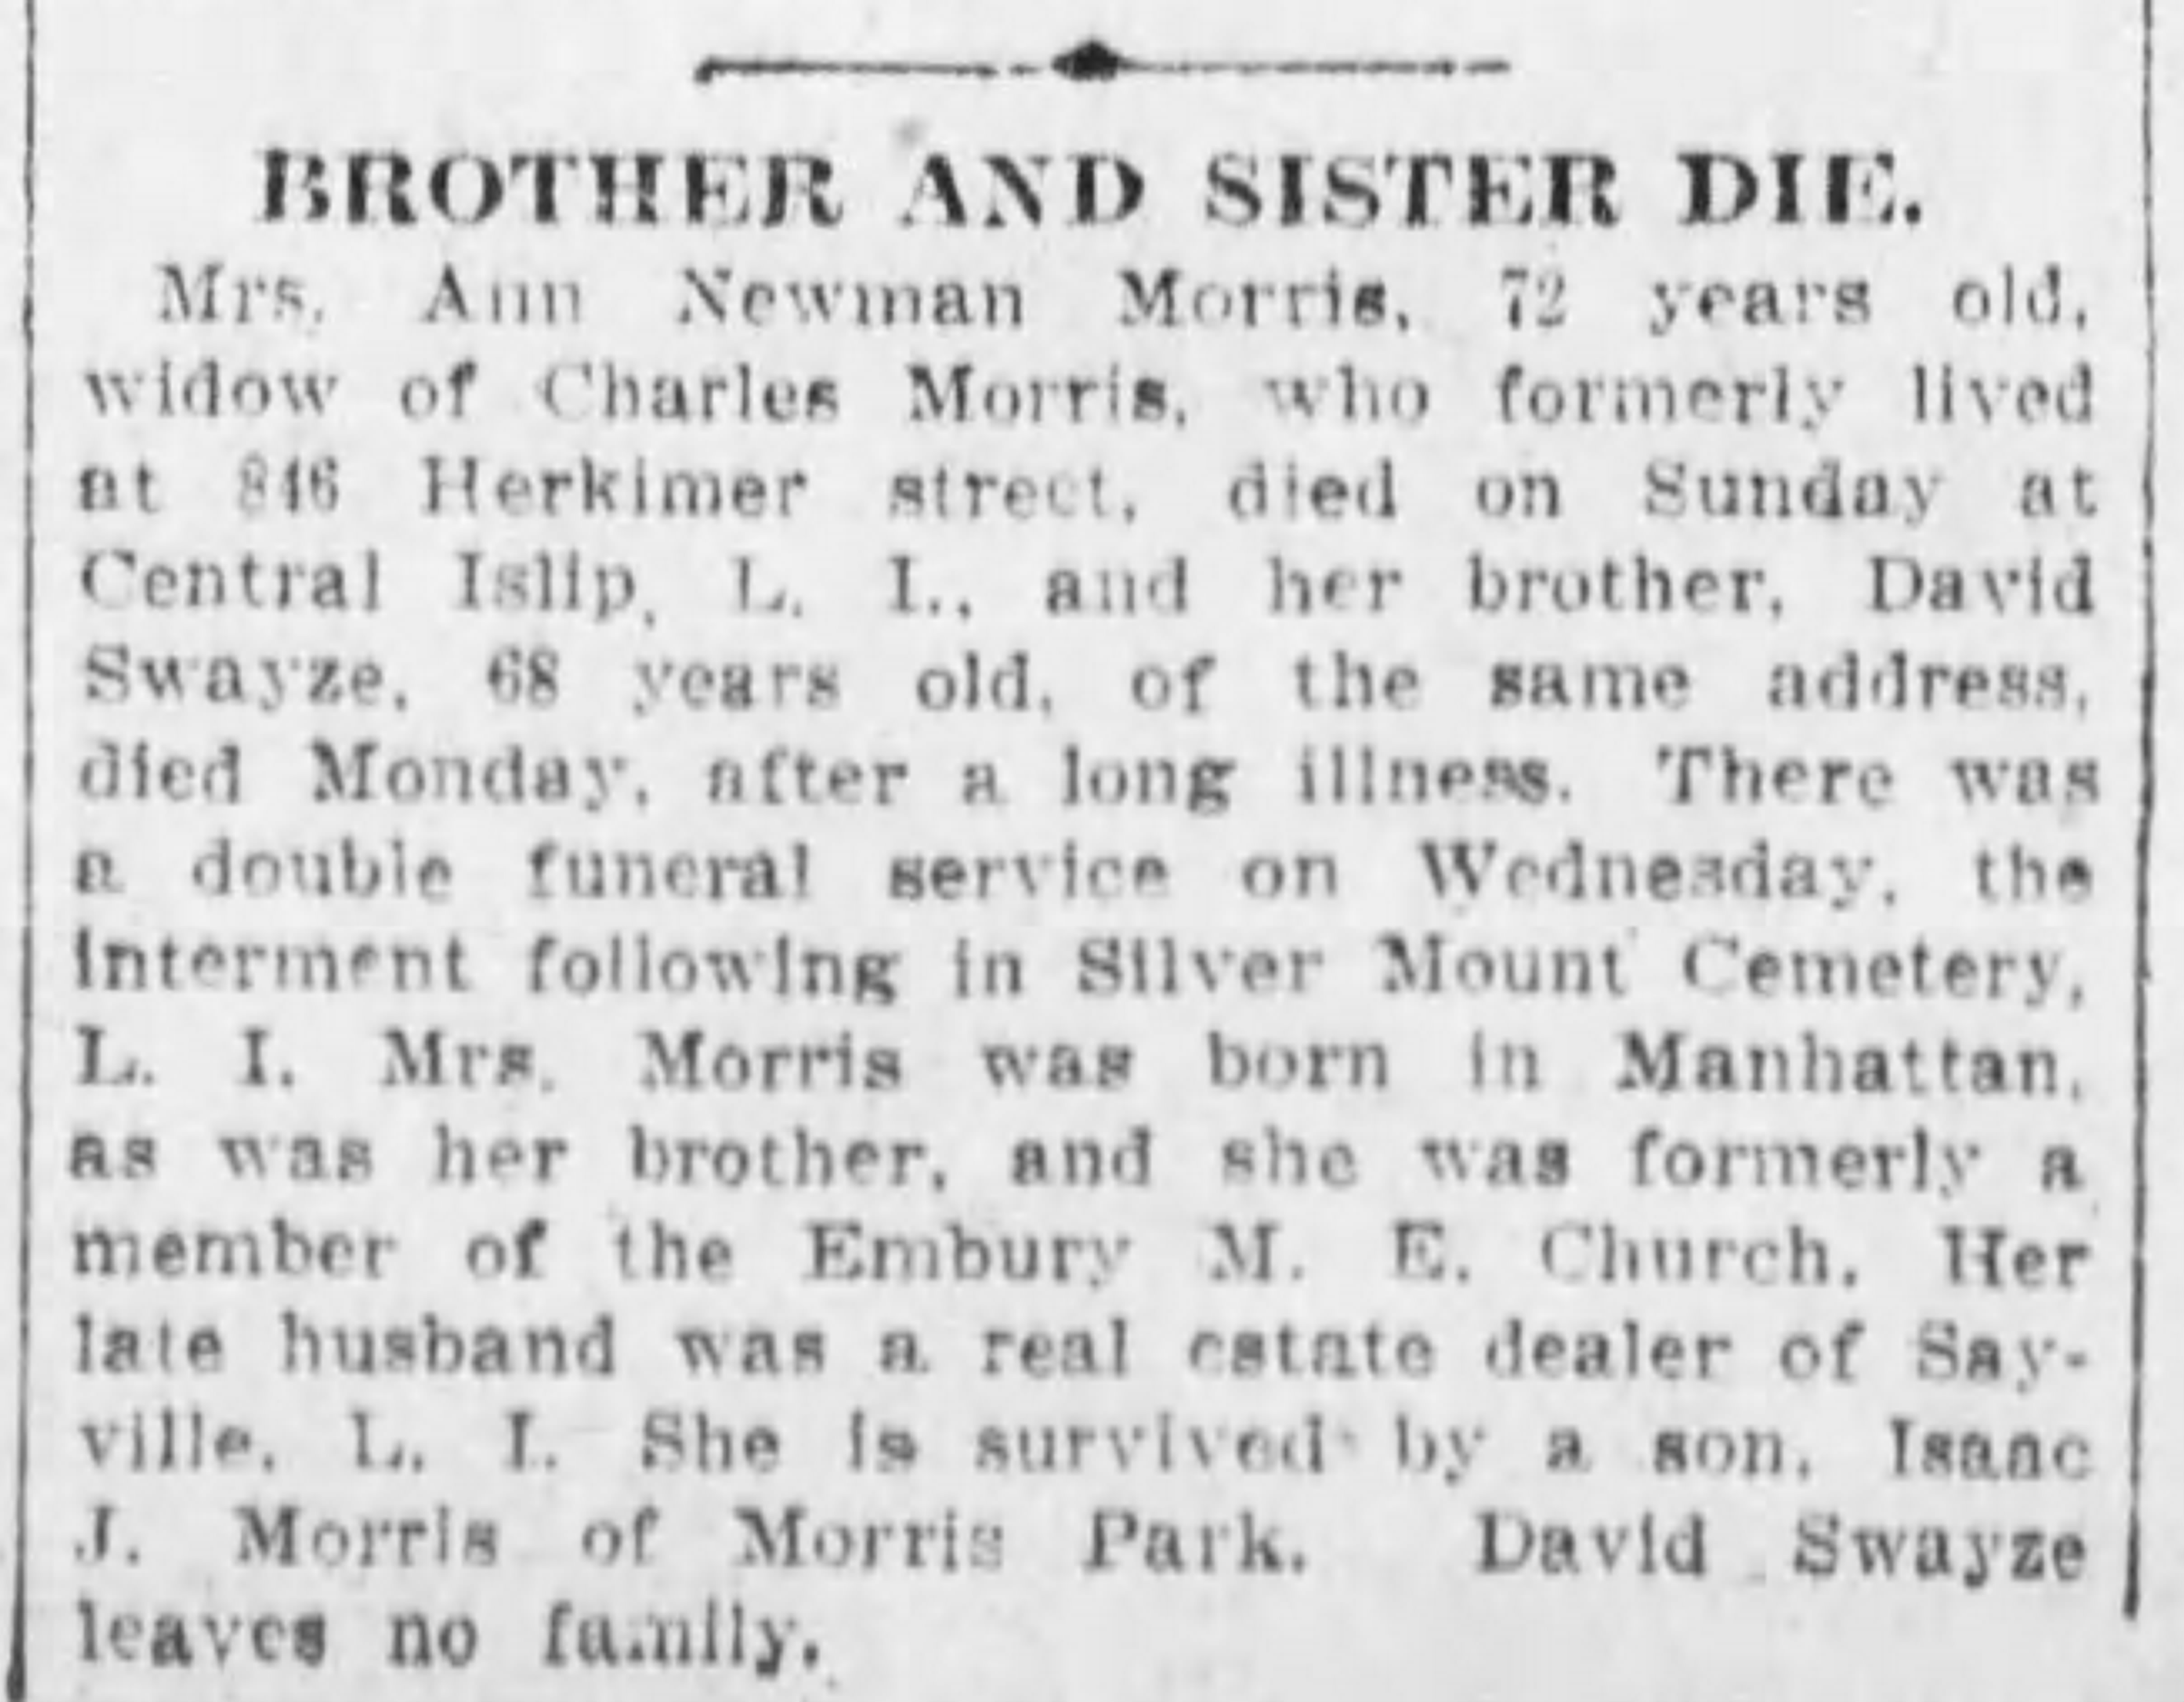
\includegraphics[scale=0.04]{images/The_Brooklyn_Daily_Eagle_Fri__Mar_16__1917_.jpg}
\caption{The obituary of ``Grandma'' Ann Morris and David Swayze in the Brooklyn Daily Eagle, printed March 16, 1917, page 8. [Source: \url{http://bklyn.newspapers.com/image/53892463/}, accessed August, 2014]}
\end{figure}

Chester had been keeping company with a little auburn haired girl Lizetta Letts for two or three years. Lizetta lived down the avenue diagonally across from our first home in Morris Park. After Chester met Lizetta, no other girl meant anything to him. They were married in 1915 in her home. It was quite a wedding. Most of our and their relatives were there. I am thinking particularly of Carrie Mather, mother's sister, her husband Raymond and their two children, Fred who was a little older than Chester and Effie, a beautiful young woman, who was about Chester's age. Fred would visit us occasionally but Effie and her father we lost track of. Uncle Raymond was a heavy drinker and years later Aunt Carrie left him and lived with the folks in Ronkonkoma as a result of that broken home. 

Perhaps because of the distance separating us, we rarely saw Mom's family. Mom had a brother, Alvie LaBonte, in Rensselaer whom I had met only once. That was when Clarence DeBevoise, Louis Pesagno, our chocolate foreman at the factory, and I spent the a weekend sightseeing in Albany. I had heard that Uncle Alvie worked with a paper manufacturing company so found his business address and dropped in for a five minute chat with him. I never met his wife or children and do not even know their names.

In 1917 Vada married Roy Rubb, a tall slim good-looking boy who lived in Richmond Hill. As Roy was not in our group of boyhood friends, I had not met him until he began courting Vada.

\chapter{The First World War}

After the declaration of war in 1917, the boys of my age were confused. We had lived in a peaceful world most of our lives. The \href{http://en.wikipedia.org/wiki/Spanish-American_War}{Spanish-American War} in 1898 occurred when we were babies and the only other military disturbance was the expedition of the United States sent into Mexico in 1916 in an attempt to capture the Mexican Bandit \href{http://en.wikipedia.org/wiki/Pancho_Villa}{Francisco ``Pancho'' Villa}, who had raided our borders. In comparison with the war that had been going on in Europe since the summer of 1914, these were mere skirmishes. Our patriotism had been fanned to a fever heat and we wanted to offer our services voluntarily. We did not want to be drafted. We wanted to choose the branch of service we thought we could be most helpful. We certainly were confused. 

In this period of indecision, I can recall the urge to toss a coin and accept its fall on joining the army or navy. One day my business took me in the vicinity of Battery Park, Manhattan. It was a bright, warm day and I stood on the waterfront gazing at the shipping in the harbor, I made up my mind that the navy was where I belonged. 

I enlisted in the Naval Reserve as a seaman third class and was called to duty as a yeoman third class and assigned to Headquarters, Third Naval District at 280 Broadway, New York City. After all the pondering and indecision, here I was behind a desk while many of my friends were in the more romantic ends of the service -- at least, I thought then that they were romantic. Later, I realized that it was fate or good fortune that kept me out of combat, but at that age pride was a factor that influenced a feeling that we were slackers hiding behind a desk.

My duties were entirely clerical. The uniform and the discipline were the only things different from civilian life. I lived at home and commuted to New York like a civilian. I don't think I looked particularly heroic in the bell-bottom pants and gob's jacket and I was very sensitive about wearing them. Even though I was living at home, it was against regulations to don civilian clothes while there or any place. During the war the uniform was mandatory at all times. By the end of 1917, I was a yeoman first class and wore three stripes on my jacket sleeve and in May 1918 was made a Chief Yeoman and proudly wore the uniform of a chief petty officer. 

In January 1918, I learned that examinations shortly would be held for a paymaster training course at the \href{http://en.wikipedia.org/wiki/United_States_Naval_Academy}{Naval Academy in Annapolis, Maryland} starting on August 1. This seemed to offer a real opportunity to get away from New York and perhaps get a commission and an assignment to sea duty. With the recommendation of my commanding officer and letters from DeBevoise, United States Title and the principal of Commercial High, I applied for permission to take the examination. Permission was granted and I took and passed the examination.

Much to my disappointment, I was not included in the Annapolis group. I did so much want the opportunity to take training in that historic academy. But my disappointment was tempered with the announcement a short time later that another training course, United States Navy Officer Material School for the Pay Corps, was to be established at Princeton University and that I would be included. Now I was happy. I was about the remove what I thought was the stigma of desk duty in the City and, at the same time had proven to myself that I could compete successfully in an effort to improve my status. It was the first real test of competitive competence outside of school and sports. My folks were proud. And I hoped a certain charming young lady I had met a short time before shared that pride. 

In the spring on 1918, Art Wenige and I dropped in at a dance for servicemen (Art was an Army trainee at \href{http://en.wikipedia.org/wiki/Camp_Upton}{Camp Upton}) given by the USO in Brooklyn. There Art met a young lady in a Red Cross Nurse's uniform. When Art suggested a date, she agreed on the condition that a friend of hers come along if I would care to make it a double date. I agreed but wondered who was being imposed on me as I had had some experience on double dates and never seemed to pick a winner. 

We kept the date. I can't remember where we went or what we did because I was in a daze. I had met THE girl -- Mabel Norseen, an 18 year old slim blond girl with a ``peaches and cream'' complexion. She lived at 563 10\textsuperscript{th} Street in the Park Slope section of Brooklyn and I can remember leaving her that night after she promised me another date and somehow or other finding my way home to Richmond Hill. I was really ``hit hard.''

I wondered what she thought about me, whether she felt that I was the ``boy of her dreams.'' I doubt that she did because I was far from a romantic figure in that gob's uniform which accentuated my thin, pale face and my slightly bowed legs. These are the thoughts that bothered me after that first meeting. But she had agreed to another date so maybe she did like me. Shortly after that eventful first meeting, I proudly called on her wearing my chief petty officer's uniform which gave me a lot more confidence in my burning desire to make a favorable impression. Maybe I did because we were together several times before I left for the paymaster's school at Princeton with her promise to write after. 

Along with 100 or more hopefuls (perhaps 200), I reported to the Naval officer in charge of training at Princeton early in September 1918. We were billeted in beautiful Graduate College at the far end of the Princeton campus and I was thrilled with the place. At long last I was at ``college'' or at least in the environment of a college. I was billeted with three other ``M's'' -- Murdock, Moses and Morrisey -- in a room in the graduate building. It was an oddly assorted group. Murdock was a Harvard man, later to become a professor there; Morrisey, a tough little Irishman from New York City; and Moses, a quiet spoken boy of Jewish descent and also from the City. 

The training was not too difficult. It consisted of lectures on navigation and on subjects concerned with naval regulations and paymaster's duties with on period a day devoted to actual military training on the parade grounds. I cannot understand why we took such military training when our jobs were to be on paper work. It must have been for the discipline factors. 

I so much wanted Mabel to come to Princeton for a weekend so I could show her the University and how we lived and studied at the College. But most of all I wanted to see her. We were corresponding regularly and had made tentative arrangements for her visit. However, her parents were very strict and she was not permitted to come.

An army officer training school, also at the University, had formed a football team and challenged the navy school. I tried to make the navy team but after a few bruising practice sessions realized that a skinny 135 pounder didn't have a chance in competition with the heavy-handed huskies on the squad. When we finally played the army I was happy that I wasn't in the game for it was a bruising battle-royal with no holds barred. The army won. They had the least number of casualties. 

A day long remembered was November 7, 1918 when word was flashed (erroneously) that the war had ended and an armistice effected. A group of us were on leave in New York City and became a part of the wildest, most tumultuous demonstration I have ever witnessed. We were in the vicinity of Times Square. Shouting, cheering and weeping crowds jammed the streets. Anyone in uniform, regardless of whether they wore service stripes, was literally mobbed. Those men in our group were embarrassed by the homage accorded us, which, incidentally included indiscriminate hugging and kissing by the young gals and by the old ones too. We were being pushed into the Hotel Astor and found ourselves at a table in the roof garden in the noisiest dining room I have ever been in.

Men in uniform could not be served drinks in a public place, but plenty were passed under the table to us by civilians at other tables. It was a night long to be remembered. It was a night which rightfully belonged to the millions of service men on the battlefields and on our fighting ships. There was a bad letdown the next day when it was reported that the rumor was false and there had not been an armistice declared. That was to come four days later on November 11. But the premature celebration was nevertheless the big one. 

In connection with the passing of drinks to service men on the night of the big celebration, I might mention that I had never tasted alcoholic beverages of any kind until I put on a uniform. Pop and Mom were teetotalers and drink in our home was not even thought of. On those prewar occasions when I was with friends in a cafe, I would order soft drinks. But when in uniform, I guess I wanted to show my independence. 

Back at Princeton we were winding up our training and taking examinations. We were commissioned on November 15 and ordered to the Naval Training Camp at Pelham Bay, New York. The final night at Princeton was a wild on. Someone started a snake dance and before it ended some 200 men were in line snaking through the rooms over the tops of anything in our way and then on out to the campus. We never did hear what action was taken on replacing the broken furniture. 

At the Pelham camp we were given time to obtain our uniforms. I went to a custom tailor (Haines Brothers) on Fulton Street near DeKalb Avenue in Brooklyn and ordered a uniform, overcoat, cap and believe it or not, a sword. Regulations at that time called for a sword as part of an officer's equipment. What we were to do with it was a big question. All of this equipment was at our own expense. 

Ten days later, resplendent in my new Ensign uniform, I reported to the receiving ship in Brooklyn (barracks on the short of New York Harbor) to await orders for sea duty. These orders did not come until nearly three months had passed. As a staff officer, my duties were quite limited during this waiting period. Once or twice a week when officer of the day, I slept at the base. I was on a subsistence allowance which meant that when not on night duty, I was given an allowance for board and permitted to sleep at home. It may be of interest to note that this allowance plus my pay as an Ensign totaled more than my earnings at DeBevoise. Because of limited facilities at the base, the officer's mess was at the nearby \href{http://en.wikipedia.org/wiki/Crescent_Athletic_Club_House}{Crescent Club} which gave me an added thrill of lunching at one of Brooklyn's finest clubs. It was quite an experience for a poor buoy and I was quite proud I will admit. 

But my biggest break of luck in being stationed in Brooklyn was the opportunity to see Mabel frequently. We were ``keeping company.'' I rather think she took some pride in introducing her officer sweetheart to her friends. I met the members of her sorority and those of her boy friends not in service abroad. I seemed to be accepted as one of the crowd. I had little time for those of my old pals who were still at home. 

Wad and several of the old Brooklyn group were in the army or navy abroad. One of his close friends, Al White, whom I had come to know very well, was killed on the battle fields. Fred Pettit, the son of our old Sunday School teacher and a charter member of our class, was reported missing in action and never found. Other friends were in the service in various parts of the world. 

A short time before the war, Wad had taken a job as a secretary with J.P.~Morgan \& Company on Wall Street. He was enlisted in the 305\textsuperscript{th} Infantry training at \href{http://en.wikipedia.org/wiki/Camp_Upton}{Camp Upton} on Long Island. After receiving basic training, he was assigned to the staff of the Second Assistant Secretary of War in Washington as a Second Lieutenant. Now in Paris with this staff he was in the type of work in which he was so well qualified. He was advanced to a First Lieutenant and then to Captain. In France, he became friendly with another member of the staff, Merle C.~Hale. After the war Merle and I became close friends -- a friendship that ripened as the years passed and was terminated by his death in 1961. 

On February 27, I received orders to report to the \href{http://en.wikipedia.org/wiki/USAT_Buford}{United States transport Buford} upon arrival in port. I checked daily but had no word of its arrival. She was long overdue. On March 9, I read the following Universal Service dispatch in the press:

\begin{quote}
``Newport News, March 9 -- After floundering in heavy seas for twenty-one days, losing her course many times in a terrific storm, the United States transport Buford, with 1025 returning soldiers on board, came into port to-day. She was towed by rescue tugs that picked her up off Cape Henry late yesterday. 

Fuel was almost exhausted and the steering gear gone when an S.O.S.~was picked up by tugs that rescued her after a terrific battle with the waves.''
\end{quote}

I wasn't too pleased with this news and wondered what was ahead of me. I took off for my assignment the next day and as it was late in the evening when I arrived I checked in at a hotel. The next morning I decided to get my bearings on the hereabouts of the ship before reporting. I discovered that the Buford was an old merchant ship taken over by the Navy as an Army transport. Alongside the trim naval ships at dock, she ever did look shabby. With the takeover of the ship by the Navy, the civilian officers had been commissioned as Naval officers. 

It was fortunate that I obtained this information before reporting for duty because if I had reported as naval regulations required with that shiny new sword at my side I think I would have been tossed overboard. I went back to the hotel, packed my gear and walked to the ship with it under my arms. I simply introduced myself to the skipper, Commander Olsen, and told him I was reporting for duty. If I had reported to that old sea dog according to regulations, I hate to think of the consequences.

Fortunately for me, a raw Naval Reserve Supply Officer, the Chief Yeoman assigned to me was a regular Navy man with many years of experience in supply practice and regulations. Like all seasoned chief petty officers he knew his job and was a fine chap. He did the work and I was more or less a figure head treading softly for fear of making myself a conspicuous neophyte. The first test of such fear came when I had to climb down a rope ladder over the side of the ship to a supply barge below. It was night and that swaying ladder seemed a mile long. With gobs watching, I managed to scramble down that later, check the supplies and climb up again without, I hoped, too much loss of dignity. 

The first night on the Buford I joined a group of officers and a civilian salesman for a game of poker at a hotel. One of them produced some liquid refreshment which resulted in more of a drinking bout then a card game. The civilian got a bit out of control and two of the officers were forcibly restrained by the others from throwing him out the window. So ended another episode in my efforts to be accepted as a regular guy by those ex-merchant sailors. 

A few days later the Buford took off for France but didn't get much beyond the harbor before there was more propeller trouble and she was forced to return to the dock. Thus ended my military duty for two weeks later I was detached from active duty and returned home on March 22, 1919. Like many, many other volunteers, we had no battle scars or had won honors in fighting. But we had gained a lot of experience which I think was helpful in the battle for business survival and progress in the years ahead. Back in civilian life I was eager to resume my old job with DeBevoise. 
% Insert footnote here that explains that the Buford actually had a decorated history after his time on it.

\chapter{Back To Civilian Life}

The transition to civilian life was a bit rough. For the past six months my commission had carried some prestige and now, so to speak, I was at the bottom of the heap again. As I needed new suits -- but more likely because I wanted to show-off -- I wore my uniform during my first week or so on the job. I must have looked silly calling on jobbers in the South Brooklyn territory wearing an ensign's uniform and lugging a big sample case or standing behind that big desk in the office posting the journals. But the uniform was soon discarded and I eased into the business grooves again.

DeBevoise had been enjoying good business during the war despite material shortages and sales were running over a million dollars a year. He was now granting monthly bonuses to the foremen and key personnel and informed me that I would receive one also. Shortly after I was given additional sales opportunities along with a used \href{http://en.wikipedia.org/wiki/Ford_Model_T}{Ford Model T}. Although it was understood that the Ford would be garaged in DeBevois's new warehouse and garage across the street from the factory, I did drive it home on those Saturdays I worked the Long Island territory and would hold it over the weekend. It was on such a Saturday that I invited Mabel to join me and we had a very nice trip together, that is until the time I thought I could look into her eyes and at the same time weave through traffic. I found to my dismay that I did not have such dual vision when I drove the Ford into the rear of a parked car on a street in Freeport with a crash heard a block away. Fortunately the car I hit was a heavy one with a strong bumper and not damaged at all. The Ford, however, was damaged severely and had to be towed to a garage for repairs while we went home on a Long Island train. The owner of the parked car evidently sense the situation and did not make any trouble for us. We thought he was a great guy. 

% Timeline: 1919

The summer of 1919 was indeed a happy one. The uncertainties of the war days were behind us and I had what I thought was a good job with good prospects. But the crowning happiness was the love Mabel and I shared. We would see each other one or two nights a week and on Sundays. If we had lived near each other I would have seen her every day. But the problem was transportation. If we were at a late party and I missed the last night train on the Long Island Railroad (1:10 am) there was a long trip via elevated railroad with a long walk on the Richmond Hill end. 

Mabel had graduated from the Brooklyn Training School for Teachers and was teaching in the Park Slope section. On Wednesdays, which were the days I worked that territory, I would arrange my schedule so that I could meet her and drive her home, the long way of course. Many Sundays we spent on the beaches with Jack Glanders and Ida Hansen or with Harry Maass and his bride-to-be, Billie. 

In the early winter of 1919, Mabel and I thought that we should obtain Dad Norseen's blessings on our intentions (although there wasn't much doubt that he and Mother Norseen had not anticipated them). So after much discussion in the parlor of her home one evening, Mabel called Dad Norseen in, told him I wanted to talk with him and left the room. I can recall that we both stood as we talked. Neither of us smiled as I stammered through a monologue of my love for Mabel and my expression of confidence in my ability to take care of her on my salary of sixty dollars a week and the good prospects ahead for me in the candy business. I also mentioned that I had a little bank account, but did not mention how little. I cannot remember whether he said ``OK'' or just grunted, but that experience was over and we were officially engaged. 

On Christmas 1919, I had the pleasure of placing an engagement ring on Mabel's finger. Arrangements were made for a wedding in October 1920. Our happiness was marred, however, by the untimely death of Mabel's 18 year old sister, Florence in January 1920 and the attack of influenza which Mabel contracted at the funeral service at the cemetery was to have serious repercussions in the first two years of our marriage. 

Meanwhile, Wad Smith had returned from his military service in Paris as a Captain and with a French bride, Marthe. They had met in Paris and had been married after a brief courtship with Wad's good friend Merle Hale, also a Captain, as best man. Marthe, a widow with a baby boy, Jack, had some difficulty with English on her arrival. We had a lot of fun with her and Wad and saw them frequently. Marthe, like so many other French and Europeans had the idea that all Americans were wealthy. As she told us later after Wad was really ``in the money'' she had her eyes opened when Wad took her to his parents' little flat and the simple bungalow they owned in Staten Island. 

Wad had accepted a job as a secretary with the General Motors Export Company and suggested that I too join up with that progressive little company. I felt, however, that the DeBevoise outfit offered better opportunities. Mr.~DeBevoise had promised that eventually he would turn the business over to his key people. I still do not know whether or not I made the right decision. Ten years later I did make a connection with General Motors but meanwhile Wad had made an outstanding success with GM. During 1920, for of reasons I do not now recall we lost frequent contact with Wad and Marthe. I think during that time he spent some time in Europe for GM.

Mabel and I were tied up with our own problems as mentioned previously and with our plans for our wedding. The big event took place at her home on 10\textsuperscript{th} Street on October 20. It was a simple little affair with only the immediate family in present -- Mom and Pop Morris, Mother and Dad Norseen, Chester and Lizetta, Vada and Roy, and Aunt Carrie Mather. Jack Glander was my best man and Hylda Booth was Mabel's Bridesmaid. Dr.~Young, Pastor of Mabel's church officiated. Jack, who had been taking vocal lessons and had a very fine tenor voice, sang \href{http://en.wikipedia.org/wiki/Oh_Promise_Me}{``Oh Promise Me.''}\footnote{Music by Reginald De Koven and lyrics by Clement Scott.} Mother Norseen served the wedding supper. It was a quiet affair but exciting nevertheless. In order to escape the rice and kidding, Mabel rode the \href{http://en.wikipedia.org/wiki/Dumbwaiter_(elevator)}{little kitchen dumbwaiter} into the basement and ran out through the front basement door to the car where I was waiting, but did not succeed in evading our well-wishers. 

Our stop for the night was the old \href{http://en.wikipedia.org/wiki/Hotel_Pennsylvania}{Hotel Pennsylvania} in New York City. Here I experienced the embarrassment of signing ``Mr. \& Mrs.'' for the first time while rice fell from our clothing. The next morning before getting up we discovered a couple of painters peering through the transom. When we left we saw that the scaffolds they had used for redecorating the halls. This served as an entertaining conversational piece with our many other newly married friends. Our next stop was a little hotel at Delaware Water Gap. Not very far from home, not very fancy and not expensive. But it was all we could afford and it seemed very wonderful to us. That October in 1920 was \href{http://en.wikipedia.org/wiki/Indian_summer}{Indian Summer} with a vengeance. We had expected crisp cool weather and had dressed accordingly. Our attempts at mountain climbing and hiking therefore were not too comfortable. Here too we found that the influenza Mabel had suffered had taken its toll as she found it difficult to climb or take long walks.

Mabel had planned to continue teaching. Her folks wanted her to capitalize on their investment in her education and to build a backlog of experience in teaching as a security safeguard in the event she needed it in future years. For that reason we had decided to live with the folks in their 10\textsuperscript{th} Street home while she continued with her teaching. We purchased furniture for one of the two bedrooms in the ``railroad'' flat and boarded with the folks on returning from our honeymoon. With board of only ten dollars a week and our combined salaries we figured we could build a little nest egg. But that thought was soon forgotten in the worry over Mabel's health. 

Her condition worsened rapidly and before the end of 1920 examinations by her family physician and a lung specialist indicated that she had tuberculosis. In January 1921, a little more than two months after our marriage, we arranged for her admission into Loomis Sanatorium in Liberty, New York. Despite rest and excellent medical attention at Loomis, her condition deteriorated. In the following June, I had a noted New York City specialist Dr.~Roy Upham, visit her at Loomis. His opinion was negative. He felt that she could not survive another two or three months. However, neither he nor the good doctors at the sanatorium had taken into account her will to live. This fighting spirit plus the artificial collapsing of the diseased lung (a new method at the time) brought a hope that was realized in 1922 about two years after our marriage. 

Meanwhile I continued to live with the Norseens rather than back in Richmond Hill with the thought that my presence might help alleviate their sorrow. For us it was a long period of alternating hope and despair. For me, in addition, it was a long period of physical as well as emotional strain. Each weekend regardless of weather, I would drive to Liberty over Rout 17 which at the time was a narrow winding road with long grades and extremely dangerous in wet weather. The old Ford had been turned in on a Maxwell roadster with side curtains which could be rolled up in sunny weather ( -- incidentally, I had to purchase this car. DeBevoise contributed only the trade-in value of the Ford). After a few months of weekend driving alone, I teamed up with Ted Lauer who was the husband of a fellow patient of Mabel at Loomis and would alternate in the use of our cars. He lived in Hackensack and many times I would spend Sunday night at his home rather than continue on to Brooklyn after a particularly difficult drive. Ted worked in the office of \href{http://en.wikipedia.org/wiki/E._F._Hutton_\%26_Co.}{E.~F.~Hutton} and in later years became a partner in that prosperous firm of stockbrokers. Unfortunately, Ted's wife died shortly after her return from Loomis. 

I do not want to dwell for too long on this Loomis episode in our lives. It is one we had to put out of our minds. It is strange that the things most of us recall are the pleasant ones and rarely think of these which have been difficult. However, I would like to mention two things that helped to soften the impact of our concern and worry during Mabel's illness. One was the overpowering optimism and cheerfulness of the patients at Loomis, many of whom had little hope of recovery. The other was the good cheer and fellowship of the husbands and relatives who were accommodated at a little boarding house on the hill at the back of the Sanatorium. Here we had our meals and comfortable beds after our long trips and short visits with our wives at the hospital. Here, too, we had interesting chats with our new friends.

It was a great day when I was told that Mabel would soon be discharged -- an outstanding example of a ``cure.'' One condition of her discharge was to live in as high and dry a climate as possible within a reasonable commuting distance from my office. After a long search for such a location, I answered an advertisement for boarders at a West Summit, New Jersey residence. It was a beautiful old home with spacious lawns and many shade trees. It was an answer to our dream. The owners, the Steidel's, a couple with three teenage children, had suffered temporary financial reverses and welcomed us to their home where we lived as members of the family for about a year. Mabel had no household obligations and plenty of opportunity for sunshine and rest. 

One hardship for me, but one I cheerfully accepted, was transportation to and from my office in Brooklyn. This included the bus from West Summit to the Summit Station, the Lackawanna train to Hoboken, the Hudson Tube to New York, the subway to Borough Hall Brooklyn and the trolley to the office. Five modes of transportation and at considerable expense. 

After a year, Mabel was able to take up housekeeping in a new apartment house at 1020 President Street near Prospect Park in Brooklyn, and within a few moments ride on the Vanderbilt Avenue trolley to my office. Here we furnished our three-room ``dream house'' and were back to normal and beginning the kind of life we had hoped to begin three years previously. Here we had the opportunity to renew friendships and family ties. 

Shortly after our return, Mabel's folks sold their 10\textsuperscript{th} Street house and moved to one on 8\textsuperscript{th} Street. Meanwhile, Pop and Mom Morris had built a small bungalow on the old ancestral property in Ronkonkoma which Pop had inherited from Grandma Morris. This was completed in 1921 on a tract of land on the north side of the track. However, Mom and Pop did not move there until a year or so later. Chester had lost his job with a textile organization and moved into the new house with his little family for the period of job relocation. He and Lizetta now had two children -- Evelyn born in 1916 and Roger born in 1920. In 1922, Pop and Mom sold their home in Richmond Hill and moved to their new home. From there, Pop commuted to his work in the Morris Park railroad shops until his retirement in 1936.

But despite the long hours of travel, Pop was happy to be back in the area of his childhood. His grandmother, Caroline Swayze had purchased the property he now owned in two parcels, one in 1856 and one in 1869. On a five acre plot she had purchased (I assume about 1860) directly opposite on the south side of the railroad, she had built a two-story frame house and large barn where, I have been told, she maintained a small estate. In the rear of the property was a family burying ground (long since evacuated) in a square of large white pines. The house was entirely destroyed by fire in 19??. 

When but a small child, I can recall frequent visits with Pop and Chester to the unoccupied old homestead and sleeping on the floor on blankets we had brought with us. We undressed by the flickering light of an old kerosene lamp casting weird shadows through the empty room and with the smell of stale air and age making our accommodations somewhat haunting to say the least. As the house was rented at times, the attic which contained many family heirlooms was kept locked. All were destroyed in the fire and I do regret that the folks had not had the foresight to preserve the old muskets and other antiques in a safer place. But what would be considered antiques today were simply ``older things'' to my folks at the time.

Pop loved the place and sorely missed the old house. Shortly after the fire, he built what we called a one-room shack (about the size of a large country chicken coop) in the orchard adjoining the site of the old house. Chester and I spent many happy weekends camping out there and playing with the children from a house which had been formerly the old Lakeland railroad station before the station stop was moved one mile east to its present location. Incidentally, Grandpa Morris was the agent of the Lakeland station for a couple of years prior to his death in 1991 and Grandma Morris continued on in that capacity for a short time after. But now I am losing the continuity of my story. I had planned to deal with events before my time in a supplement to this. 

The little old shack which housed us on those happy weekends was moved across the tracks in the oak grove and became one of three Pop built for campers and to make a little extra pocket money. I think his little shacks were among the forerunners of our modern motels. After Mabel and I had resumed ``normal lives'' again, we visited Ronkonkoma frequently. Many such visits will be mentioned as we get along with our story.

As I mentioned earlier, Mother and Dad Norseen had sold their home on 10\textsuperscript{th} Street and were renting. They missed the pride of home ownership and suggested that perhaps we could pool our resources and build a house. In the spring of 1925 we planned such a home and bought a lot on East 23\textsuperscript{rd} Street in the Flatlands section of Brooklyn. Dad knew a Swedish builder who we called in for consultation. He secured an architect and a contract was drawn up for a two family house -- five rooms and bath on each floor with a spacious cellar and toilet. As I had had little time to accumulate savings since Mabel's illness, Dad and Mother agreed to take up a second mortgage for us. So we were on the way toward home ownership, and for Mabel and me a heavy burden of interest and amortization charges with little money left for other things. We got a great kick from watching the house grow during that summer and fall. We literally inspected every piece of material going tino its construction. It really was a well built house, not because of our careful watch but because we had an honest builder. Mabel did a good job, too, in shopping for furnishings and interior decorating. The house was completed in December 1925 and we celebrated our first Christmas in that new home of ours at 1627 East 23\textsuperscript{rd} Street, Brooklyn. 

To all young people comes a great feeling of pride with ownership of their first home. Such pride in my opinion is greater only in the marriage ceremony itself and in the birth of the first child. To Mabel and me, one of the two greater feelings of pride -- the birth of our boy -- was to be withheld for several years. We were proud of that house. It was a palace in our eyes. Our parents were just as proud and happy. But I think their happiness was a reflection of our own. All parents want to know that their children are happy and gain happiness themselves through that knowledge. We do not realize that fact until we are parents ourselves and feel, telegraphically it seems, the happiness or unhappiness of our children. 

In the new neighborhood we made new friends and continued also to keep in close touch with old friends. Sally (Lund) Upham, a friend of Mabel since childhood, lived a block away on 22\textsuperscript{nd} Street. She introduced us into a group of young couples living in the neighborhood and we were welcomed into the fold. The men of the group formed a ping pong club and played one night a week alternating in the basements of those who had tables. It was not long before I, too, had a table. To this day, we speak of these friends as the ``ping pong'' crowd.

Shortly after we took up residence on East 23\textsuperscript{rd} Street, Wad and Marthe Smith bought a small one-family house nearby on East 16\textsuperscript{th} Street. Wad was climbing rapidly up the ladder of business success in General Motors and his work took him abroad frequently. When he was at home, however, we saw him frequently and had many good times together. They now had two boys, Jack who was six or seven years of age and Edgar who was a small baby just a few months old. They also had a young colored maid. At that time this was a real indication of affluence. The maid, Ida Winters, remained with the Smiths until after Wad's death many years later and was a real ``mammy'' to their children. 

In our new neighborhood, many of the girls of Mabel's sorority, and their husbands of course, lived nearby. Likewise, two of my old Richmond Hill friends, Harry Maass and his wife Billie, were conveniently close. Thus, we were in a wide circle of good companionship and caught up in a social life which we thoroughly enjoyed. It was not a pretentious social life by any means because we were all young married couples who had to watch the pennies. Despite the pitifully small amounts we could afford for social activities, we were rich in friendships. It was my opinion then, and still is, that aside from one's family, the greatest assets are a person's friends. They and members of the family provide the little world around which everything else revolves, and in the bigger world we call the Earth there are millions and millions of such compact little worlds in which inhabitants reap rich dividends in the form of love and friendship.

Now with additional expenses of the new home and expanding social obligations, I simply had to continue to attempt to build sorely needed material assets. I applied myself with even greater intensity to my job. It seems that when most discouraged with my progress and the progress of the business, I worked harder. Perhaps I was more loyal to the business than to myself. Through mail courses for home study and consistent reading of \href{http://en.wikipedia.org/wiki/Printer's_Ink}{Printer's Ink}, the ``business bible'' of that period, I sought the academic learning of business that I had missed. Looking back, however, the opportunity of becoming familiar with all areas of a small business together with the opportunity to understand people through contact with people in all phases of work in the plant and with the varied personalities of my customers gave me a broad practical education that stood me in good stead in later years. At the time, however, it seemed I was moving backward instead of forward. 

With the death of one of our older salesmen, I took over a part of his territory -- Philadelphia, Trenton, Southern New Jersey, Bridgeport, New Haven and some nearby areas. At the same time we inaugurated truck deliveries to Philadelphia and New Haven. This gave me the opportunity to increase our business in those markets because the customers would have no freight charges but we would have the expense of the haulage. A market cultivated for years by a man who had the respect and confidence of the trade is not easy for a new man to work. This I found out after a couple of trips. 

Fortunately, I met a fellow salesman, Charlie Schwartz, who lived in Philadelpia and was a son-in-law of the owner of the Goldenberg Candy Company, manufacturers of \href{http://en.wikipedia.org/wiki/Goldenberg's_Peanut_Chews}{Goldenberg's Peanut Chews}. Charlie was very popular in the trade and he took me ``under his wing'' and opened many doors of customers that would have been difficult for me to do at so early a time in my venture in that market. We became very friendly. I rode with him in his car when I worked the Philadelphia and Southern Jersey market, and we with me when he worked the markets in my home territory. Often times I would stay overnight at his home and would reciprocate by having him at my home. But in those first years in the Philadelphia market, I put  up in the old \href{http://digitalcollections.nypl.org/items/510d47da-550b-a3d9-e040-e00a18064a99}{Green's Hotel} which has long since been torn down. In our Southern Jersey trips, Charlie and I would stay at a hotel in Bridgetown, New Jersey. 

The New Haven-Bridgeport territory was a difficult one to work largely because I did it in one Saturday a month. With road conditions as they were in the mid-twenties it would take me three hours to reach New Haven -- and that with fast driving on those stretches of the old Boston Post Road where conditions permitted. As my first appointment was at 9 am, this meant that I would have to leave home at 6 am and after working New Haven, Bridgeport and Norwalk, arrive home at nine or ten o'clock at night. There could be no social activities for us on those Saturdays. These trips were particularly difficult during the winter months with snow and ice slowing us down. As can be seen from this illustration of my work, long hours were the rule rather than the exception, and to heighten my discouragement, DeBevoise's business was slowly declining. As conditions worsened with no hope of increasing my earnings, I took on Peanut Chews as a side-line and managed to pick up a few extra dollars in commissions.

Mr. DeBevoise had held out the hope over the years that he would eventually give the business to his key men. This expectation was the lure that kept us working at an abnormal pace. In 1927, after returning from my Philadelphia journey, I was told that he had held a meeting with key men and offered to \textit{sell} the business -- not including the buildings -- for \$100,000. I was also told that I was inculded in the group and would be appointed sales and advertising manager. I thought that now we could inject new ideas into the organization and really make some money. I was keen to take that gamble even though it meant an initial endorsement of \$5,000. [Illegible] My problem was to raise my share of the down payment. I had no cash. I approached a boyhood friend who I knew was making considerable money in a business he had taken over from his father and developed into a nationally known organization. To my surprise, he pleaded lack of funds. Finally, I reluctantly went to Pop and Wad Smith. Wad loaned me \$3,000 without a question, but Pop could only afford \$1,000. Despite my limited income, the notes were paid off at six percent interest within three years. It was a real struggle to meet those obligations and it could not have been done without the cooperation and sacrifices of Mabel. She made her own clothes and kept our household expenses at a bare minimum. At one time she sold magazine subscriptions door-to-door.

Our hopes for injecting new ideas into the company did not materialize. My associates were older men, steeped in the traditions of the past and unable to recognize the changes that were taking place in our industry -- changes that demanded new concepts of products and markets. As a result of this failure on the part of my partners to take action to meet new needs, the business went from bad to worse. By mid-1928 our sales were down to a half million dollars and I was selling one half of that total. The situation was bad and I was driving myself at a pace much too fast to be continued. 

The situation in which I found myself was ironic. Here we were near the tail end of the ``roaring twenties'' which will go down in history as a period of post-war inflation, rising costs and wages and wild speculation. With the exception of a brief recession in 1927, the country was prosperous and business in general was booming. These conditions were the source of our problem in the penny candy business. The value of money was declining as it always does in inflation and the penny was insignificant and in reality replaced by the nickel.

Grocery, cigar and 5 and 10$\cent$ chain stores were expanding in numbers and absorbing the business of the small stores. Five cent bar candies as well as package and bulk candies were on the counters of these stores and at reduced prices. The little candy stores (and the little grocery stores, too) were fast disappearing -- and with them our major market. 

With the thought that it might not yet be too late for a final attempt to make my associates understand the need for a major readjustment of our business, I started work on a detailed survey and analysis of our business which would support recommendations for needed action. This was an exhaustive study of product and market trends over the years. It took many hours of my ``spare'' time to get together the facts on production and sales of the more than one hundred manufactured items to make the accurate and convincing analysis of the need for action to save the business and move ahead to new goals. 

But, again, my associates were reluctant to face realities. They could not understand the facts of business life and still hoped for a miracle restoring old trends of consumer demand. The only solution for me was to get out of the business and seek a connection with a more progressive organization. I had been in business for 16 years (including two years in war service) and never had to look for a job. I became an avid reader of the classified section of the New York Times and spent my Sunday afternoons answering ads for sales executives in all kinds of business and mailing personalized form letters to a long list of companies with whom I would like to connect. However, few were interested in a fellow whose products were sold for pennies. 

One that held the most promise was an interview with the [Illegible], at the time a sales leader in the high-grade package trade. My appointment for an interview was set for a Friday afternoon in a suite at a New York hotel. Unfortunately, that was a day I was returning from Philadelphia where I missed my train and arrived panting and perspiring an hour late for the interview. I was received courteously but coldly by the President of the Marketing Manager. It was quite evident right at the start that I would not receive favorable consideration because of my tardiness. After the interview I received the usual polite note telling me that the job had been filled. 

Another interview was with an executive of General Foods with [Illegible] Francis who later became Chairman of that Corporation. I liked Mr.~Francis and would have enjoyed working for him but it was the policy of General Foods to have all their sales personnel start at the bottom as truck route salesmen. As the pay was about half of my pay at DeBevoise, I could not accept the job and still meet my financial obligations and maintain our existing living standards.

Just about the time my discouragement was at the lowest possible depth, I had the idea that if my survey and analysis of the DeBevoise business was as good as I thought it to be, there was no reason why it could not be used as a selling tool in my job search. I typed copies of the study and mailed it with t a covering letter to the \href{http://en.wikipedia.org/wiki/Young_\%26_Rubicam}{Young and Rubican}, a young and progressive advertising agency, and to \href{http://en.wikipedia.org/wiki/General_Motors}{General Motors} Export Company. General Motors was also a young and aggressive organization and from the stories of my two friends, Wad Smith and Marle Hale, was destined to be an outstanding industrial organization. Wad was Assistant to the President of the Export Company and Marle was Personnel Manager. Here was a situation that appeared to be made to order for me. But the big drawback was my friends. Because I was in a business entirely unrelated to automobiles and with a yearly volume equal to the daily volume of the Export Company, they felt I could not measure up to the standards of their organization. They were afraid to recommend me. They had their own reputations at stake and any failure on my part would be a reflection on their judgement. 

Both had discussed their thoughts with me and I knew just where I stood. As a matter of fact, I had given up all hope that I would get into GM. However, I did not realize the effectiveness of that Survey and Analysis. One of them, never found out which one, showed my letter and attachment to the President, \href{http://en.wikipedia.org/wiki/James_D._Mooney}{James D.~Mooney}, and he was interested. Now, my friends had the go-ahead. Late one night in mid-August, I received a telephone call from Merle telling me that I had a job and after the preliminaries of filling out application forms I was to start work on September 16, on Mr.~Mooney's staff at a salary of \$400 a month, which was fairly substantial in those days. the job was ``special studies.'' I could be thankful indeed that I had toiled so hard to prepare that survey. And this thankfulness was doubly felt with the receipt of a letter from Young and Rubican requesting that I drop in for an interview. They were seeking a man to go into the plants of those of their clients where there seemed to be deficiencies in products or sales and make recommendations for improvement. In other words to do what my survey was planned to do for DeBevoise. 

With the GM job assured, I was faced with the problem of breaking the news to my associates at DeBevoise and making arrangements for the return of my investment. My departure would be a bad break for them, not only because of the sales I was bringing in but also because of the fact that my contract specified of the repurchase of my stock. The Company could ill afford this additional financial loss. As there was no cash, I agreed to take a series of notes calling for monthly payments to me. Despite their unwillingness to appreciate the true situation regarding their business practices, I felt a real pang in leaving them. Four years later the business failed, thus confirming my appraisal. I was the only member of the rim to recover my investment.

\chapter{Beginning at General Motors}

After a short vacation, I reported for a new job at GM on September 16, 1929. It is a coincidence that I started my job with DeBevoise on September 16, 1912 and as I note these facts the date of this writing is June 16, 1963.And this sixteenth of June is an historic date because it is the 73\textsuperscript{rd} anniversary of the marriage of my parents. An event which sparked the beginning of our generation of the Morris family -- Chester in 1891, James (Alfred) in 1893, Vada in 1897 and Kenneth in 1908. This anniversary date stirs memories of many happy reunions but let's leave that in the interest of continuing my business story. I will deal with those occasions in a later section. 

On that morning of September 16, 1929, I entered the General Motors building with considerable trepidation. How could I, a man from little business, fit into this big business organization? How could I compete with the men who had helped to make it grow to such a size? But I had asked for a job and here I was on the threshold of what could be a new and exciting career. So buck-up, old man, keep your eye on the ball and show them you can compete. Such thoughts were interrupted by a warm greeting from a personnel man, Bill Winslow, who ushered me into a big window corner office on the 17 \textsuperscript{th} floor containing two desks -- one with a name plate block reading ``James A. Morris.'' I was thrilled to say the least. Compared with my cramped quarters in front of the dirty sink and behind that old stand-up bookkeepers desk in the DeBevoise office this was just too good to be true. But there was a name on the desk. Maybe, those last few years in the candy business were a nightmare and I had awakened in the office where I belonged. 

I was introduced to Joe Fischler, who headed the special study group of the President's staff, and a couple of the men working for him who were to be my new associates. The walls of Joe's office across the corridor were lined with progress charts of all kinds and all with the trends pointing upward. I was given an armful of pamphlets, reports, memos and studies to read and told that I would be left alone until I had had time to acquire a sophistication of the business. 

The Export Division was in a cycle of tremendous growth under the able leadership of its president, James D.~Mooney, and an executive group of aggressive, business-advertising young men (the majority about my own age). In less than a decade, the Division had become a major competitor in those countries where automobiles were manufactured -- England, france and Germany -- and was well entrenched in other European countries and in New Zealand and Australia and had pioneered in what were in reality virgin markets at the beginning of the decade. In 1929, the Export Division included 19 oversees assembly planets, five warehouses and three distributing companies. Business was running at an annual rate of \$300,000,000. Furthermore, in 1925 GM had acquired \href{http://en.wikipedia.org/wiki/Vauxhall_Motors}{Vauxhall Motors} in England and at about the time of my arrival were negotiating for the purchase of \href{http://en.wikipedia.org/wiki/Opel}{Adam Opel} in Germany. 

This was the outfit a starry-eyed youth from the penny-candy business had joined. But it took only a day or so to realize that those outstanding results had been accomplished not by supermen, but by men like those in small business. The only difference was that these men in the Export Division with the backing of a powerful parent company had been encouraged to use their good common-sense abilities in reaching the goals set for them regardless of any obstacles, financial or otherwise.

The story of the development of GM abroad illustrated with case examples of the venturing and daring of young men given the responsibility for building markets abroad would read more like fiction than fact. However, in that first week with the Division, I got the impression I was associated with a lot of screwballs. Later, I realized that progress had been so rapid and successful as to be almost unbelievable. Management had to pause and pinch itself so to speak. [Illegible]. Studies and analyses were under way in all departments with the special study group occupied with some which seemed to me to be far outside the area of practicability.

I had but a few days of initiation into my new work before I was requested to join the Export Division's first Transportation Conference -- a school for instruction in transportation engineering for more efficient truck and bus merchandising abroad. A large part of the Division's sales were commercial cars and buses, particularly in those countries where conditions were not conducive to extensive individual ownership of motor cars and where rail transportation had not been developed. Trained transportation specialists would help assure the Division's continued capitalization of the urgent need abroad for the mass transportation of goods and people. About 25 men were included in the Conference. Some were from the overseas plants, some from the home office and some newly hired.

The Conference opened with meetings in New York on September 24 and left that night for Detroit for visits to the Proving Grounds, Research Laboratories and GM plants in the area. On September 30, regular sessions began at the GM Truck \& Coach Company plant in Pontiac, Michigan. Along with most of the members, I took up quarters at the Pontiac Hotel and began to acquire some practical sophistication of the automobile business through technical lectures, talks by plant and home office executives, plant visits and casual conversations with the members of the Conference who had seen service abroad.

In the organization scheme of the Conference I was appointed Chairman of the Entertainment Committee and a member of the Sales, Publicity and Coordination committees. As head of the Entertainment, my first job was to break down the formality of the foreign members so that they would mix more freely with others and omit the bow and ``mister'' when spoken to. This was accomplished by a party with generous servings of ``prohibition'' punch made with liquid ingredients purchased from a third floor tenant of an apartment house in Detroit. ``Go to Apartment D on the third floor at this address and ask for Joe. Tell him Tom sent you and he will sell you some really good stuff.'' Those ingredients, plus a half crate of oranges and other ingredients supplied by the more affluent members of the group made a punch that helped the foreigners to remember first names of the others and to forget the courteous bow when spoken to. We had no problem of formality after that party. We also had more formal dinner parties with plant executives and arranged a golf tournament and the forming of a bowling league. Various organizations of the Pontiac plants invited us to join them at dances.

During a visit to one of the GM plants in Canada, the manager invited us to a plush country club. Aside from the old Crescent Club in Brooklyn at which I dined while an officer at Bayridge Naval Receiving Ship, this was the only other club of its kind that I had had the opportunity to visit. As a neophyte I was impressed and thrilled. A thrill I have not since experienced at the many other such places I have had the priviledge of being a guest during my long career with General Motors or on vacations with Mabel in the United States, Canada or abroad. 

At the time I had been requested to join the Conference, I wondered if I was one of those selected for the job of transportation engineer abroad. Such thoughts were dispelled by a suggestion which tied me in directly with the New York office. This was to report to New York my observations on the progress of the Conference. I was cautioned to keep the reports confidential and not let anyone know I was writing them. This was a situation I did not like but as a new employee and desperately anxious to make good, there was no alternative. So my weekends in Pontiac were spent in preparing and typing the reports. I did not pull any punches but reported candidly on procedures, progress and morale. 

Living at the hotel was rather boring and two of my new and close friends, Donald Wood and Henry Maginetti had taken rooms at a nearby apartment house. I decided to do likewise and arranged to have Mabel join me. In my absence she had been staying with her Aunt and Uncle Andrew Johnson in \href{http://en.wikipedia.org/wiki/Northport,_New_York}{Northport, Long Island}. We had a small two-room apartment in the same building with Don and Henry, both of whom now had their wives with them. Marguerita Maginetti was a beautiful and vivacious Cuban girl about ten years younger than Henry. They had arrived from South America where henry had been with GMAC. We had a delightful time with them. Henry was a good pianist and spoke several languages. 

The country was extremely prosperous during most of the 1920s. Business activity since 1922, with minor downtrends in 1924 and 1927, was high. Reflecting this high level of business, the stock market was climbing a ``boom or bust'' trend. At the beginning of 1929, the hope of quick riches had resulted in speculative excesses with bootblacks\footnote{Another word for shoeshiner}, clerks and other low income earners participation -- and largely on margin trading. Despite definite economic danger signals, optimism prevailed until that dreadful day -- October 24 -- stocks tumbled drastically and marked the beginning of a trend that halted slightly in the fall of 1931, then continued downward to mid-1932.

During this period, business activity followed a like trend. We were in one of the most sever depressions the country had ever experienced. Many businesses went bankrupt. Speculators' fortunes were lost and bank failers added to the woes of rich and poor alike. 

Because motor cars were its principal products, General Motors business, quite logically, suffered badly. In 1929, the Corporation's sales reached a peak of 1.5 billion dollars. By the end of 1932, sales had shrunk more than 71\% to a total of about 432.3 million dollars. In that three year period, employment in General Motors declined by more than 50\% and payrolls by about 62\%. In the first few months of the depression, few could conceive its duration and severity. 

Within a few days after the initial stock market break, I received a telephone call asking me to pack up and return to New York. I surely thought that this meant the end of my dream of a new career. However, I was not fired. Years later and after my retirement, Merle Hale told me that when my name was included on a list of prospective dismissals Mr.~Mooney said I should be retained ``because the organization needed men who knew how to pinch pennies.'' He had probably recalled my Survey and Analysis with its suggested recommendations for cost savings which at the time must have seemed to him to be minute. So, once again, that memo had been my good luck token.

As the Corporation had a considerable investment in the training of much needed transportation engineers, the majority of Conference members were sent to their assignments and a few of the newer employees released as conditions worsened. Back at my desk in New York, I resumed my work in special studies on the President's staff. Mr.~Mooney was also a vice president of the Corporation and many of the studies were concerned with domestic affairs. My initial project was an investigation of the desirability of an institutional show room on Fifth Avenue -- a prestige show case for the Corporation's products. My report recommended such a showroom but because of a broad expense retrenchment program, it was not presented to the Corporation for approval.

Retrenchment was the order of the day in all areas of the business including compensation. By the middle of 1932 my salary had been cut by \$1020 a year. It was not until January 1935 that a raise of \$1300 brought it back to, and a little above, my starting salary in 1929. Mabel and I did not feel any undue privation. Prices of food and goods had also declined and our standard of living had not changed to any great degree from our lower income during the last few years of our candy business experience. 

A new life was unfolding for Mabel and me. Because of the depression, we were concerned with the uncertainties of the future but not nearly to the extent we were while in the candy business. The fact that I had weathered the first storm in the new job and apparently had been accepted as a member of the team in big business gave us renewed confidence. There were to be many disappointments and frustrations ahead but our optimism in 1929 prevailed as we felt more secure than we had in the past several years. 

With Mom and Pop Morris living in Ronkonkoma, their home had become the focal point for family reunions. The pleasant oak grove on the property was an ideal place for picnicking. Most of the family lived nearby. Kenneth was living at home with the folks. After his graduation from Sayville High School, he secured a job with the Supply Department of GM Export in New York and like Pop was commuting to work. Vada and Roy lived in Smithtown where Roy was manager of a chicken farm. They had two lively youngsters, Miriam, born in 1920, and Donald in 1922. Chester and Lizetta lived in Bellerose where he had bought a house. They also had two children -- Evelyn, born in 1916, and Roger in 1920, the same year as Miriam. Following a number of jobs with Wall Street brokerage houses, Chester was with the \href{http://en.wikipedia.org/wiki/Federal_Reserve_Bank_of_New_York}{Federal Reserve Bank of New York} in New York. Mabel and I in Brooklyn were within an hour and a half drive (over the highways of today, the trip can be made in less than an hour). 

I think that my brothers and sister will agree that our family in those years experienced the maximum togetherness. We had our parents and at that period of our young married lives, the family was a close-knit unit. As in all families, however, with the passage of years and as the families of the children mature and in turn have families of their own, each becomes a unit of togetherness of its own. This is true particularly after the passing of our parents and we become the ``old folks'' and heads of our own family units -- children and grandchildren. It is a natural evolution of family life with no loss of love within the original family but with the newer units becoming the absorbing interest.

My I say here that few children realize the debt they owe their parents until they have married and established homes and families of their own. The comes the full realization of what their parents meant to them in their developing years -- the sacrifices they made and all of the things they did to mould character and integrity in their children and help them become good men and women. 

At our ages, it was this realization that drew us to Ronkonkoma and to enjoy getting together with the family on anniversaries or whenever we wanted to. The 40\textsuperscript{th} anniversary of the marriage of Mom and Pop on June 16, 1930 was such an occasion. It was a delightful affair and one long to be remembered. And there were to follow eleven more such anniversaries with Mom and Pop being honored. After Mabel and I had moved to our new home on East 23\textsuperscript{rd} Street in Brooklyn, Mom and Pop were with us on Christmas days. We were hosts to Mother and Dad Norseen also on those days. 

\begin{figure}
\centering
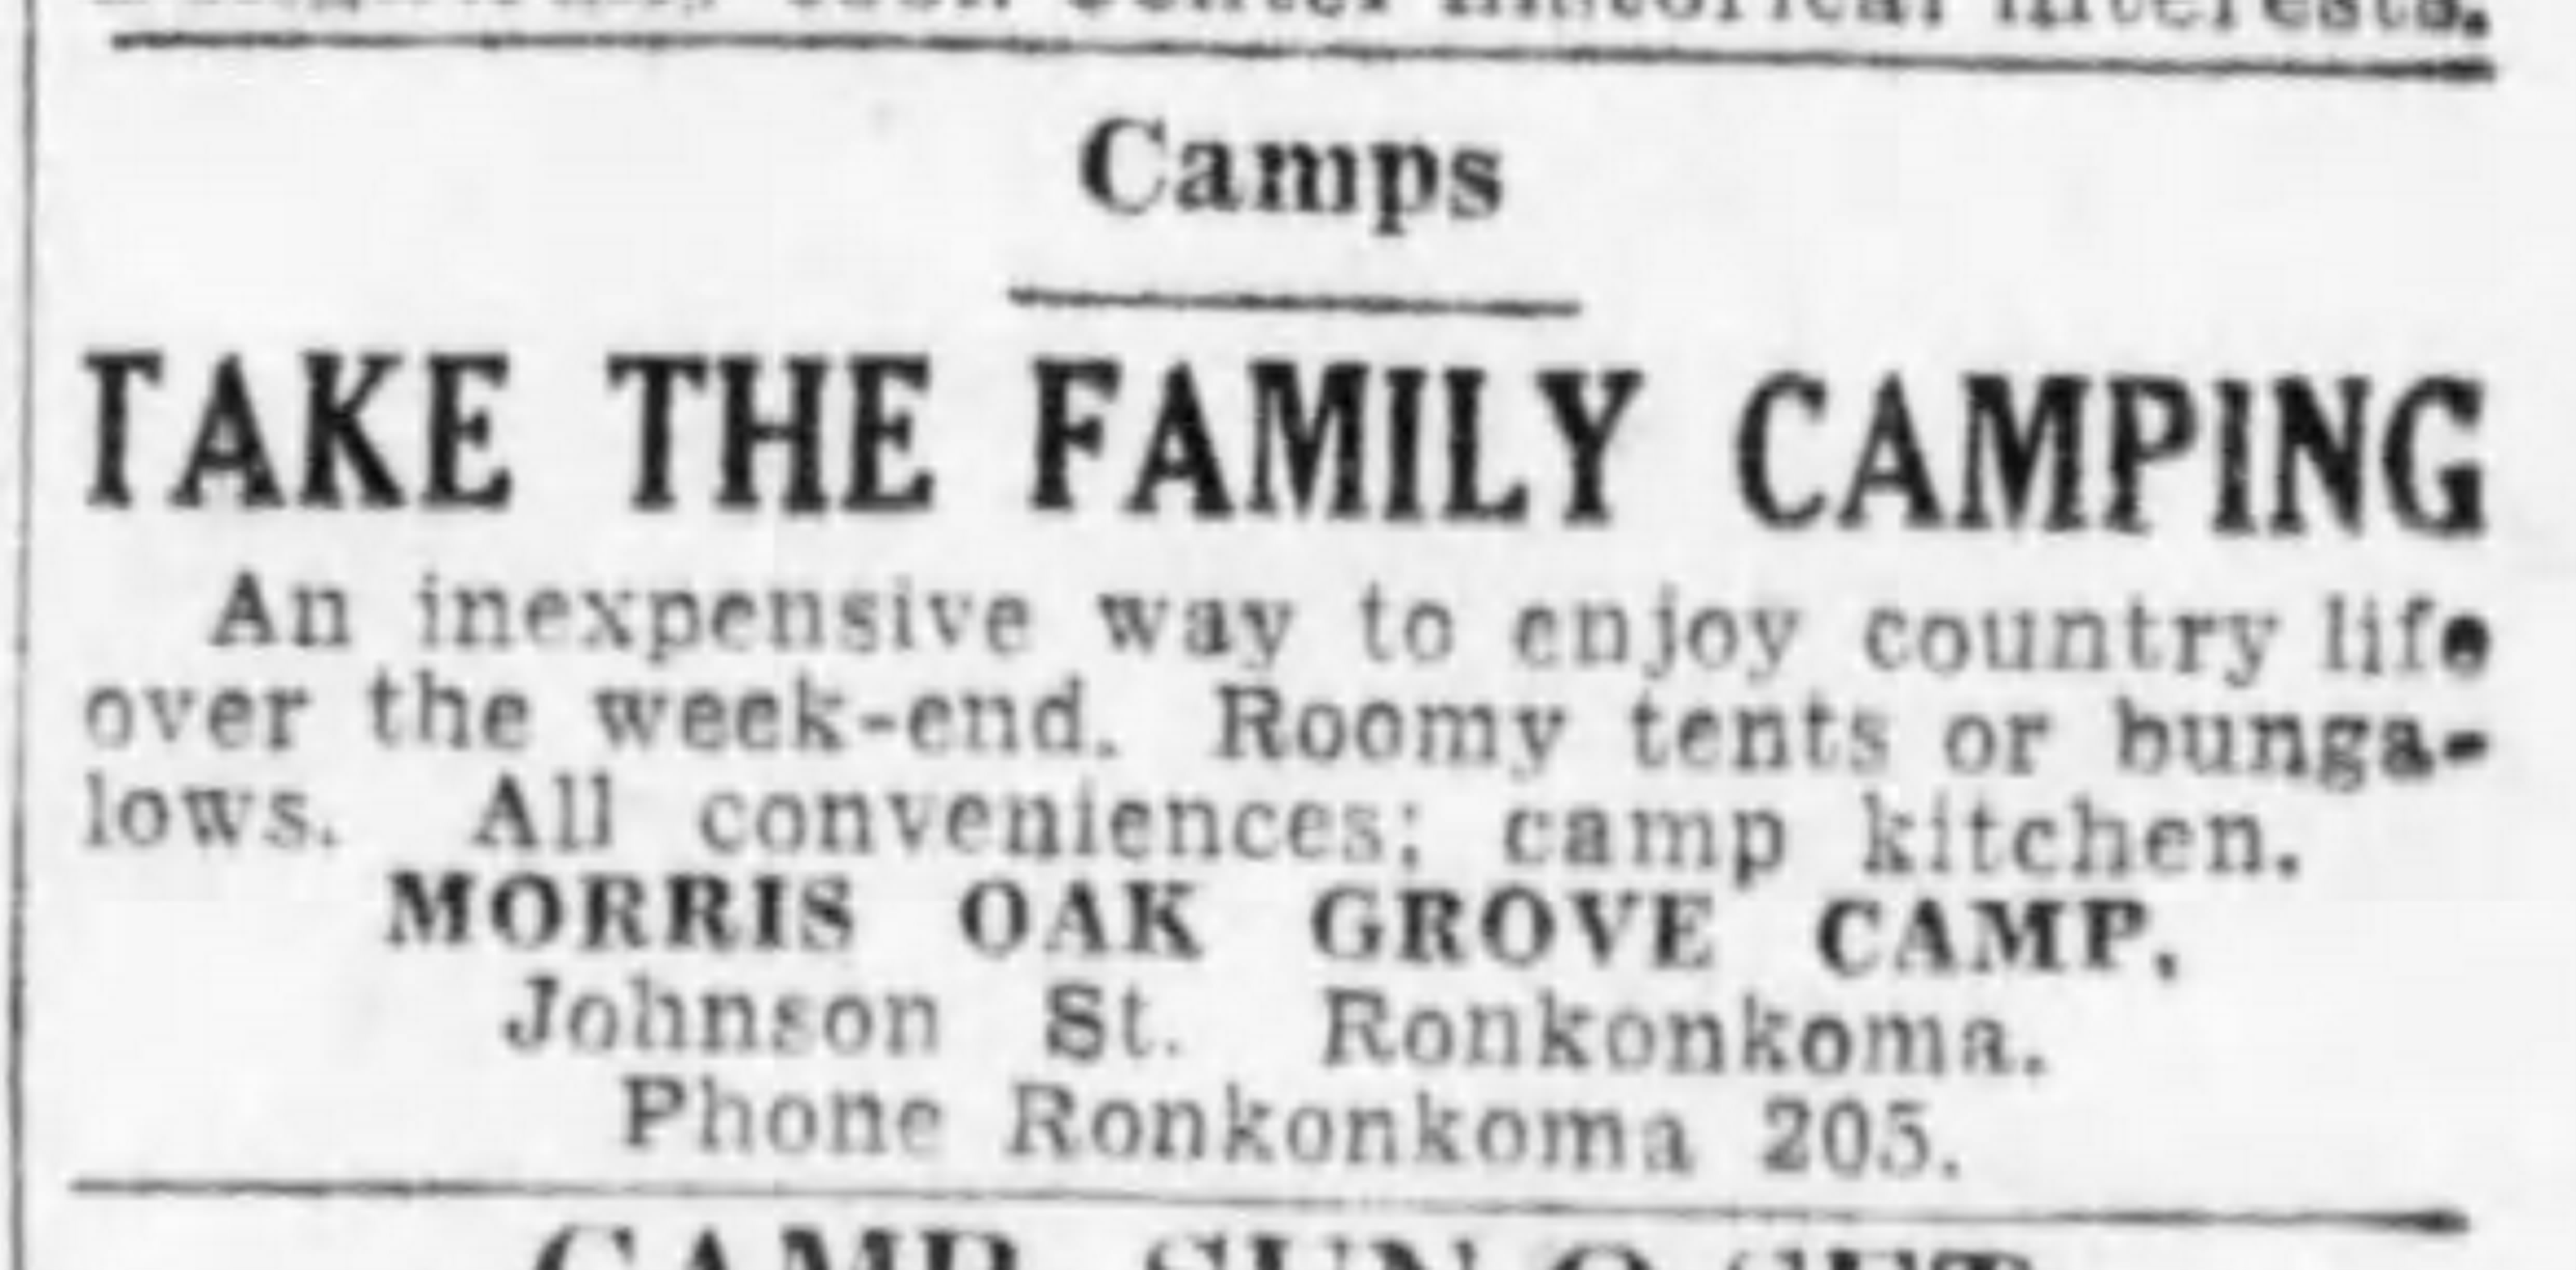
\includegraphics[scale=0.03]{images/The_Brooklyn_Daily_Eagle_Wed__Jun_17__1931_.jpg}
\caption{A classified advertisement for Isaac Morris' ``Morris Oak Grove Camp'' from the Brooklyn Daily Eagle, printed June 17, 1931, page 26. [Source: \url{http://bklyn.newspapers.com/image/58263154/}, accessed August 3, 2014]}
\end{figure}
In 1930, or perhaps a year or so earlier, Pop put up a sign in the grove ``Morris Oak Grove Camp -- Comfortable Camping.'' The camp was built around the little shack he had built on his property across the tracks and moved to the grove. Another little smaller place was built together with two wooden platforms on which he erected tents. This was the camp. I still have a letter head I designed showing the same wording and including a partial picture of the camp in which were two little boys -- Roger and Donald -- in the foreground. There was a lot of extra work involved in maintaining the camp and with only meager earnings for Pop and Mom. Some of the campers became close friends of the folks and returned year after year. 

Kenneth, meanwhile, had fallen in love with a young Sayville School teacher -- Alice Sisson -- and decided to build a house in the grove alongside of the folk's house for their first home after marriage. He and a young architect friend planned and built the house themselves. They were both out of jobs. Kenneth had felt the full impact of the depression at General Motors and like many other young men without experience found it difficult to land another. The house they built was very comfortable and good looking. It had four rooms and bath. The outside was made of California redwood logs. On July 1, 1933, Kenneth and Alice ``eloped'' and were married in Harrison, New York. Meanwhile, Kenneth had secured a job with the South Bay Water Company in Patchogue as a helper. A job which often times required him to dig ditches for the laying of pipes. Roy, who had been with the water company for a couple of years, was his first boss. As will be related later, Kenneth moved up rapidly and at this writing holds an important executive post with a successor of that company. 
\begin{figure}
\centering
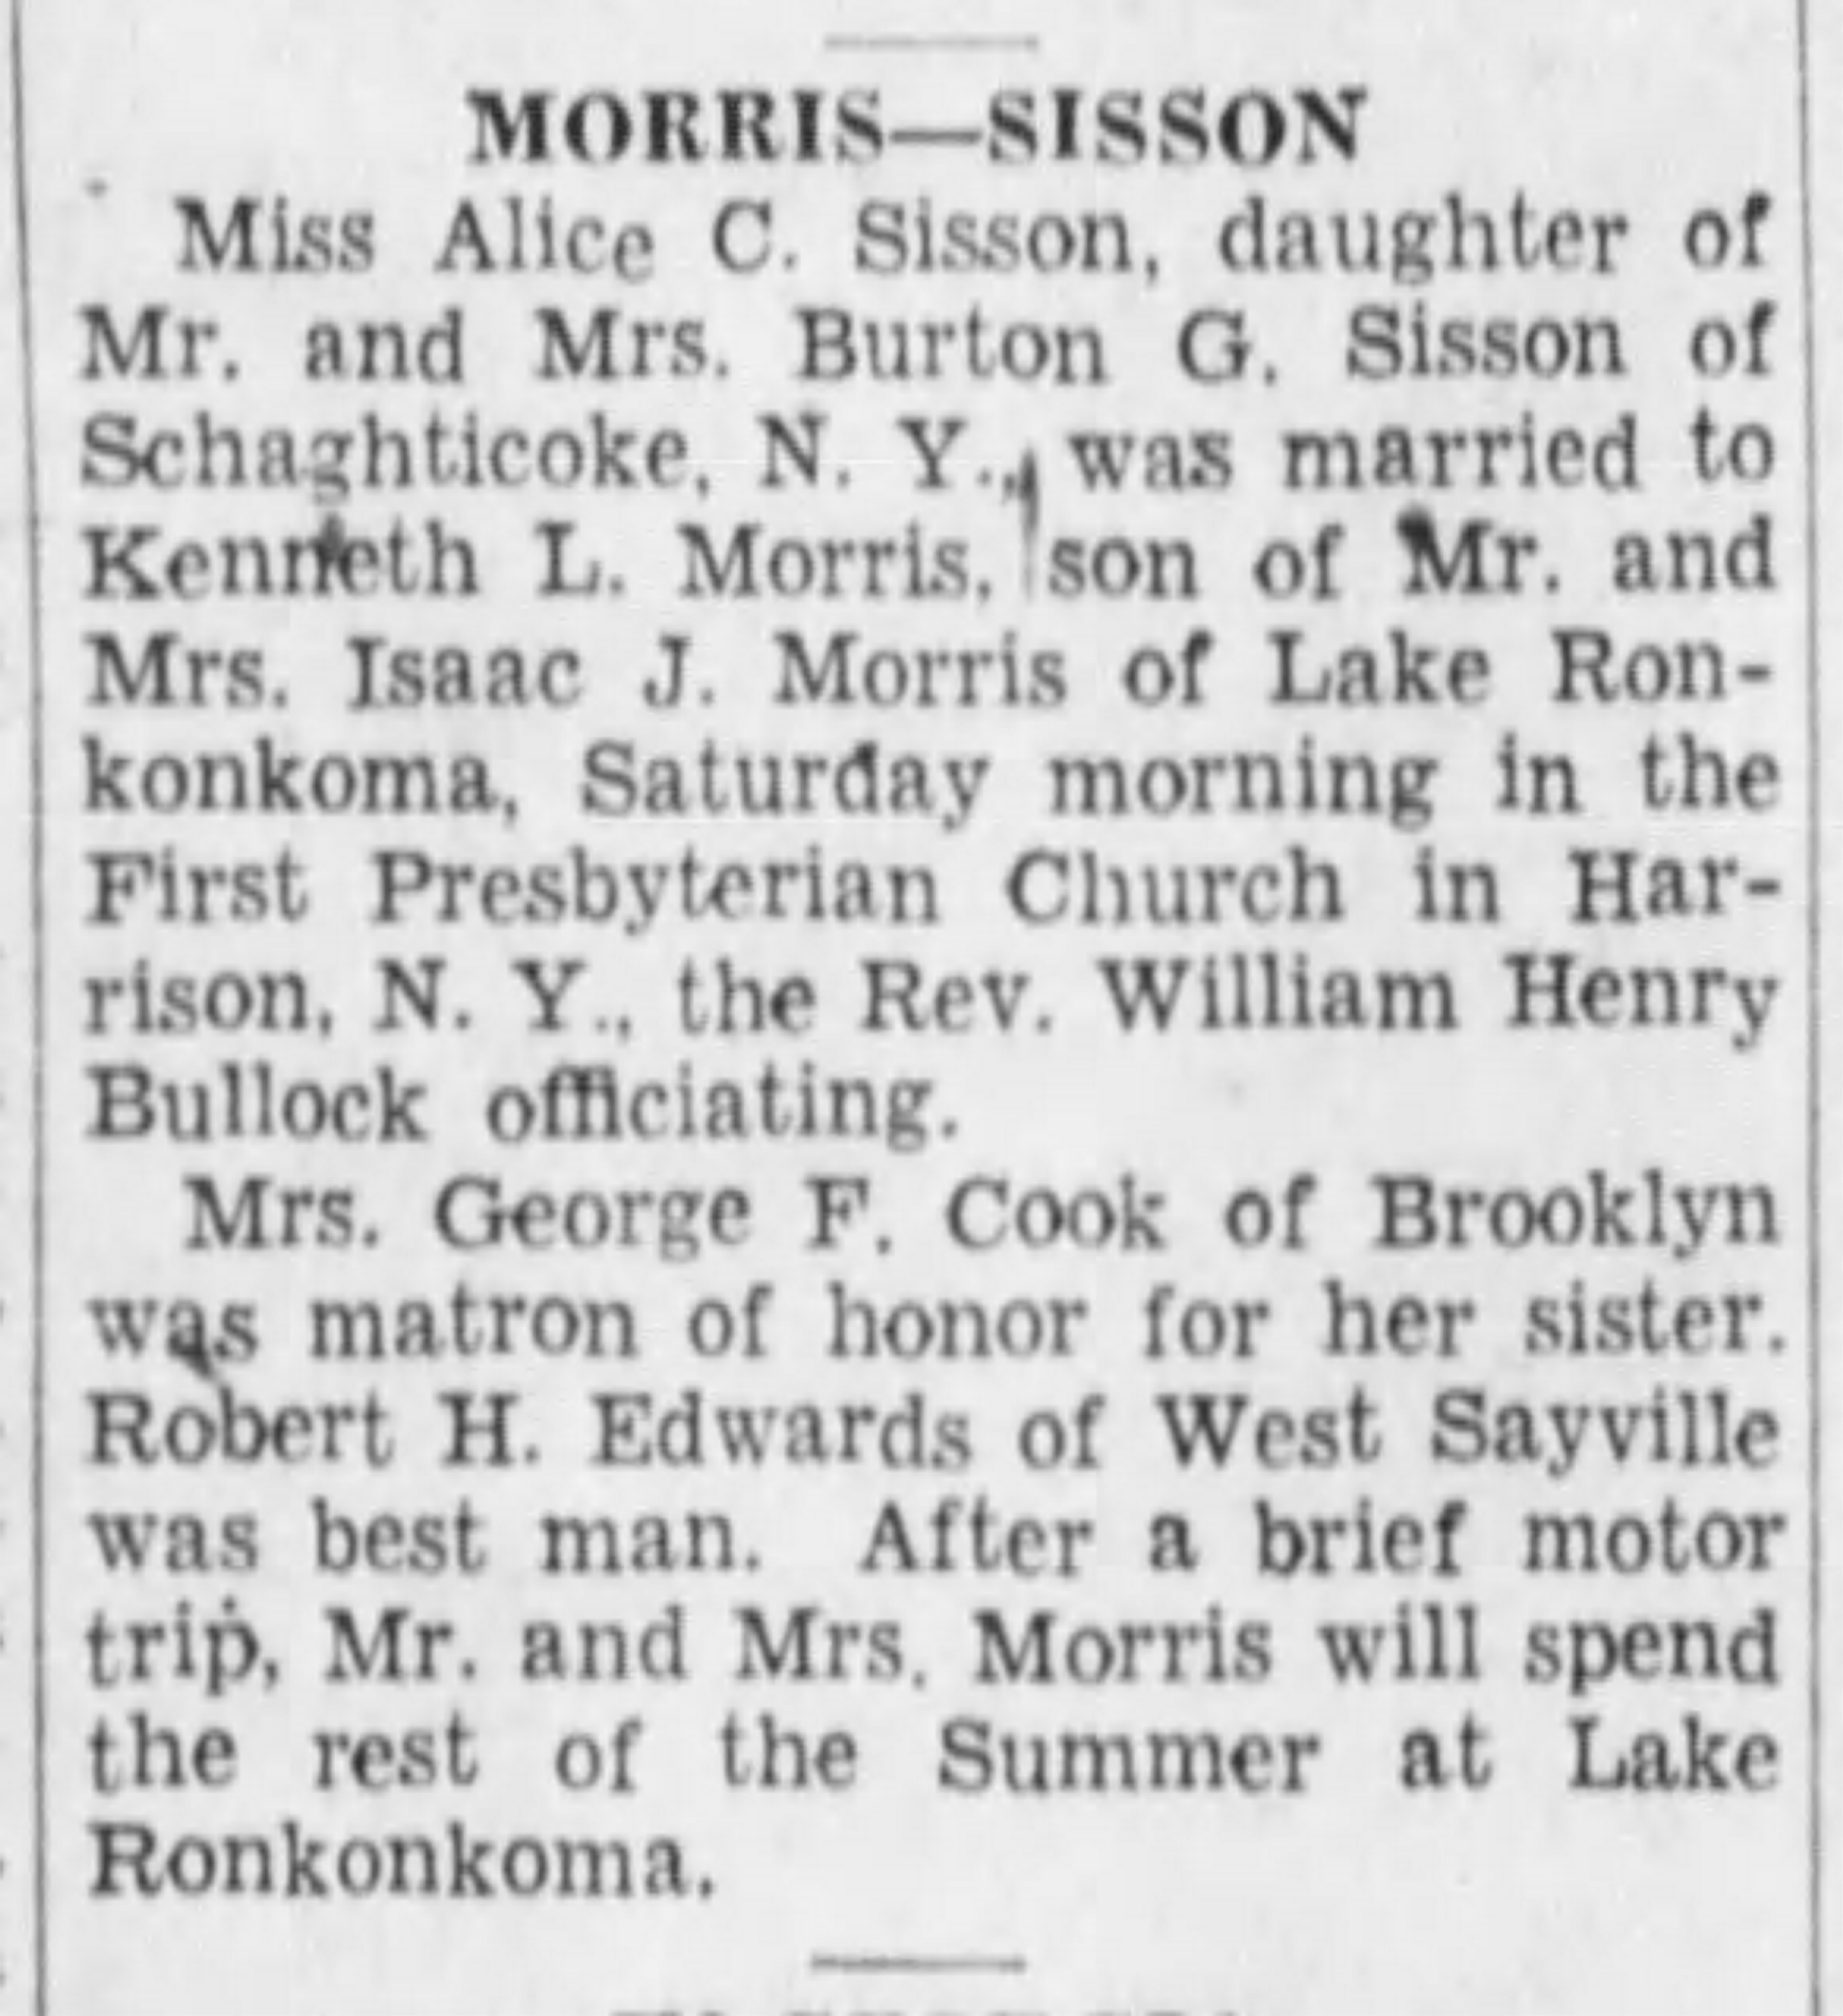
\includegraphics[scale=0.03]{images/The_Brooklyn_Daily_Eagle_Mon__Jul_3__1933_.jpg}
\caption{The marriage announcement of Kenneth Morris and Alice Sisson from the Brooklyn Daily Eagle, printed July 3, 1933, page 15. [Source: \url{http://bklyn.newspapers.com/image/59844125/}, accessed August 3, 2014]}
\end{figure}

All of the family were elated about the marriage and the fact that Kenneth and Alice were living next door to the folks. Mom had been lonesome in Ronkonkoma. She had left her church and friends in Richmond Hill. While she had made new friendships, new friendships formed in later life are seldom as close as the old ones. Now, with her youngest son and Alice, whom she liked very much, living alongside of her she was much happier. 

In Brooklyn, Mabel and I were quite busy in social activities. In addition to our local group, we were now involved with Wad's friends, mostly GM people, in Maplewood, New Jersey. We had built a large and beautiful home in that village on a large plot with many trees and a brook. Merle lived in Nutley, New Jersey, which is about a half hour drive from Maplewood. Both Wad and Merle were ``in the money,'' so to speak, as were most of the others of their group. Mabel and I, income-wise, were at the bottom of the heap. While the others had been profiting by the outstanding prosperity of the period, I had been in a profitless business. They had not yet felt the full impact of the depression. 

As a consequence, the social life we had been initiated into was somewhat hectic and wild. Entertaining at the home of both Wad and Merle was on a lavish scale. Often times, we would start an evening at the home of one and end up at the home of the other. And with all this, we worked hard at our jobs. Our fully-packed briefcases were always at home with us and after such evenings, with the prospects of the job ahead of us the next day, we would open our briefcases and go to work regardless of the time of night.

In those days at the end of the post-World War One inflationary period, it seemed to be the natural thing to play just as hard as you worked. That philosophy was followed largely by those young executives who had ``rode the wave of business prosperity'' and had gone up the ladder of business success very rapidly -- sometimes too rapidly. Only the strong could survive such a pace. The weaker ones, physically, had to choose which course to follow. If the emphasis for them was on play, then there was little hope that they could work hard. With the worsening of the depression, however, the pressures of the job -- the holding of the job, itself -- did not permit one to play hard as there was little energy left to do so. 

\chapter{Fatherhood}

Wad had three young boys -- his stepson, Hack, Edgar and Robert. Merle had a daughter, Jane, and most of our other friends had had children for several years. Mabel and I were the exception and had become resigned to being childless. But toward the end of 1932 we discovered that the stork was on the way with a package for us. However, the discovery was not made until a ``get-rich-quick'' doctor had operated on Mabel for an alleged tumor. This deception caused us much anxiety and concerned as to its effect on Mabel and the unborn child. Later efforts on our part to hold the doctor accountable were without avail. The medical profession had a code of its own.

On the afternoon of July 28, 1922, when Mabel heard our child knocking on the door, I drove her to the Midwood Hospital in Brooklyn. The following morning -- July 29 at 8 am -- a lusty boy weighing nearly eight pounds came into the world to bless us. During that long night I do not know which of us had the hardest time bringing James Alfred Morris Jr., into the world. I had not left the hospital all night, and like all near-prospective fathers, not knowing what was going on upstairs, really did have some fearsome thoughts. However, Mabel did all right without my help. And we had a son -- James Alfred Morris Jr., whose mother was 34 years of age and his father, 40. We were very, very happy. 

Unfortunately, the operation plus the not-too-easy child birth hit Mabel rather hard. After leaving the hospital she was confined to bed at home for a couple of weeks. We secured a nurse to care for Jimmie and had her with us for several weeks. When she left, we hired a maid to take care of the house work and had a succession of maids over the next eight or nine years. (In 1933 our first maid received wages of \$20 a month. In 1963 comparable help would cost between \$125 and \$150 a month.\footnote{For a still more recent reference, \$1,168 in 2014 has the same buying power as \$150 did in 1963, according to the \href{http://data.bls.gov/cgi-bin/cpicalc.pl}{Bureau of Labor Statistics CPI Inflation Calculator}.})

I don't think any of the younger married couples were more happy than we were with the birth of a first child. Like them, we had to learn to do a lot of necessary things -- to get up in the dead of night in answer to a cry without stubbing your toe against a bed leg, to hum softly and harmoniously when trying to quiet the baby, to heat a bottle at just the right temperature and to shake the milk on your wrist to be sure it is, to use unintelligible baby talk, to push a baby carriage around a corner without upsetting it, and to change a diaper without sticking a pin into the baby. To this day, Mabel declares that I never learned how to do any of these things properly, particularly in the diaper department. Maybe she is right, but I tried hard. 

Like all new fathers, I wanted to be able to give our son advantages that were not available to me and determined to apply myself even harder to my job. But that was difficult to do because I had been working just as hard as I could. Fortunately, on July 1, 28 days before Jimmy was born, I had been transferred to the Corporation as an assistant to Mr.~Mooney who was the [Illegible] executive in charge of the Overseas Operations and I had received a small raise in pay. This new assignment seemed to be a recognition of my efforts and certainly boosted my morale. However, the trend of the economy was still uncertain and business weak. One never knew when further expense retrenchments in the business would be necessary. It was a case of working hard to retain a job rather than to go forward.

The services of my good friend, Merle Hale, along with those of many other good men had been terminated. In Merle's case, however, another opportunity was made available through the good offices of \href{http://en.wikipedia.org/wiki/William_S._Knudsen}{William Knudsen}, President of General Motors. Mr.~Knudsen had observed the work of Merle and evidently liked it. He suggested that Merle take a job in the plants on the assembly line and in various other unskilled labor jobs to obtain a first-hand sophistication of the labor end of the business. Merle donned overalls and worked in the factories for a year. After that stint, he was placed in charge of personnel in the Detroit office. Later, he returned to the New York office in charge of the Corporation's Salaried Personnel Activity with an office and large staff on the executive floor of the building. He had pulled himself up by his boot straps, so to speak, and was making good -- and in a big way. 

While in Detroit, on December 19, 1933, a human-interest article on Merle appeared in the Birmingham Journal. The reporter had been attempting to interview him for a long time. In the interview Merle said, among other things:

\begin{quote}
``The things we like best about Christmas is that it prompts us to turn back the pages and live over again the many pleasant times we have had with our good friends. For example there are friends in Export -- what a fine crowd they are. Even though we got kicked out of the Export picture, we still like them and although it has been two years since we came to Detroit our interests still go back to Export. Of course, we don't see as much of them as we wish we could but someday we hope to take some time off and really make a job of visiting.''
\end{quote}
I was proud to be among those friends that Merle referred to. 

Since returning from the Transportation Conference in 1929, I had been on special assignments, a job classification that could include almost anything. In my case, they included special studies, special and routine correspondence, statistical market analyses, ``ghost'' writing of executive speeches, as well as special projects of many kinds. All of these required frequent contacts with officials and heads  of the various departments. There was considerable prestige attached to members of the President's staff and this prestige opened doors for me that would not have otherwise been possible. This was a great asset to a newcomer in the business and helped me obtain a broad background of Company policy thinking in a relatively short time.

Many of the studies I initiated myself based on clues on management thinking picked up in my contacts with executives. For example, the problem at the time was how to overcome the market leadership which Ford had enjoyed for so many years. The base of Ford's publicity was Henry Ford himself. He was dramatized as the pioneer of mass production, the friend of labor through his policy on wages, the benefactor through his preservation of Americana, a symbol of humanitarianism in business. As I pointed out in my study in 1930, Ford had created an image that:

\begin{quote}
``The Ford Motor Company is not just a huge, cold combination of men and machinery but an organization of men gainfully employed in creating a product for the common good... Ford's philosophy that the foundation of society consists of the men, the means to grow things, to make things, and to carry things has undoubtedly exercised a most profound influence on public opinion... In contrast, the bulk of the publicity finally obtained by General Motors is based on its stock market activities and its financial reports. Because there is no human or dramatic appeal in statistics, the public looks upon General Motors as a purely stock-holding organization primarily concerned with profits and loses sight of the fact that it is the parent company of all of our divisions.''
\end{quote}

Then I suggested means for humanizing the Corporation through publicity management personalities such as \href{http://en.wikipedia.org/wiki/Alfred_P._Sloan}{Alfred P.~Sloan Jr.}, and \href{http://en.wikipedia.org/wiki/Charles_F._Kettering}{Charles Kettering} and also that we adopt a General Motors insignia to be displayed on all divisional showrooms and in all advertising of General Motors and its divisions to bring home the fact that they were all a part of the General Motors Family. I do not know what section was taken on the study. But I do know that it was read and action taken on one part, at least. Four years later at a management conference, a vice president recommended that ``We should stress the name of General Motors over the countryside through unified insignia in dealers' store fronts to make the name of General Motors as conspicuous as the name of Ford.'' This recommendation was adopted and an insignia designed which has been in use since then.

This is cited not only as an example of the type of work of a staff assistant but the anonymity under which he works as well as the influence he may have in sparking an idea. I have seen recommendations in many other such studies come to light and promoted moths or years later. It may seem at the time that one's efforts are not recognized. But a good staff man realizes that he is but a member of the team and can neither ``call the signals'' nor ``carry the ball.'' What he can do is to keep on trying to sell his ideas and by so doing promote the interests of the team, and indirectly his own interests. For his own future is dependent upon his thinking capacity and his ability to get a job done. 

Even though I had proved in the candy business that I could sell merchandise, I discovered that I was a very poor salesman of myself and my ideas. Perhaps this was because of my new environment in big business and feeling that I was handicapped by lack of academic education. I still held in awe the men in the upper levels of the business with whom I was dealing. THere is no doubt that I had an inferiority complex which may have been reflected in my contacts with these men as a lack of initiative or just plain ignorance. Because of this my job was doubly difficult. It wasn't until I had been with General Motors for a few years that I overcame this feeling and met my business seniors on a man-to-man basis.

Fortunately, Mr.~Mooney was a fair-minded boss, a tough operator but just and understanding. On certain studies, he would ask how I was coming along and suggest that I work with him at his home in \href{http://en.wikipedia.org/wiki/Centre_Island,_New_York}{Center Island, Oyster Bay}. He would invite me to ride home with him in his chauffeured car for dinner and the night so that we could get started early the next morning in a little office he had set up on the shore of Oyster Bay on his estate. One such study, ``The Economics of Automobile Distribution,'' involved several such visits for work at his home. 

Looking back over the years, the sequence of events do not always fall in their proper place. The purpose of the mention of certain of the events is to present as broad a picture as possible of my job and the economic environment in which business operated at the time.

The great depression of the early 1930's which followed the postwar boom of the 1920's was not confined to the United States alone. It was world-wide. BEcause of the decline in foreign trade, there was an acute shortage of foreign exchange. Many nations as as a consequence were forced to curtail their imports through embargoes, quotas, clearing arrangements and other import restrictive measures. Economic nationalism was the order of the day with each country attempting to live within itself. This policy of enforced self-containment further softened their economies because of the shortages of goods they needed and which they could neither manufacture nor produce within their own countries. 

In some cases, private enterprise resorted to barter arrangements with private enterprise in another country in order to promote their own businesses and provide needed products to others. One such instance of barter was between General Motors and private interests in Denmark with the cooperation of our plant -- GM International -- in that country and the blessings of the Danish Government. As noted in the following quotation from the August 1935 issue of the General Motors World, this was one of the projects delegated to me. It involved the bartering of fish for automobiles. 

\begin{quote}
``Fish-mongering is about as far north of automobile marketing as it is possible to go, yet International has probably done as much investigation of the market for various types of fish as has any single fishing enterprise. Its explorations into the intricacies of catching and marketing have reached from Iceland to South America. The latest venture involves the cooperation of International in a halibut expedition to Davis Strait and extensive activities on the part of J.A.~Morris in New York. Of course General Motors itself is not engaged in the actual business in any way but, if the organizers of this expedition succeed in marketing the contemplated catch, it will net International about 200 import permits for sorely needed and otherwise unacceptable American Cars.''
\end{quote}

The growth of economic nationalism presented an additional setback to world trade and a continued threat to world peace. In many countries which did not possess the necessary resources for self-containment, the effort to become economically independent led to near impoverishment and revolution. Secretary of State, \href{http://en.wikipedia.org/wiki/Cordell_Hull}{Cordell Hull}, under President Franklin D.~Roosevelt, recognized the situation and sought support for United States leadership in bringing about a freer interchange of goods between nations through reciprocal trade agreements. Powerful interests in the United States which had long been exponents of protective tariffs were opposed to such a move. 

However many large companies, including General Motors, were far-sighted enough to support the program. Mr.~Mooney and Wad Smith in cooperation with the Foreign Trade Council, The \href{http://en.wikipedia.org/wiki/Automobile_Manufacturers_Association}{Automobile Manufacturers Association} and various other national organizations interested in world trade worked unceasingly to bring about a better public understanding of the need for action. 

I was fortunate to have had a part in these efforts through assisting in the preparation of speeches, booklets and other publicity. I also attended meetings of the various organizations in New York, Detroit and Washington. I was given the opportunity to prepare the initial draft of the booklet ``Foreign Trade and the Domestic Welfare'' which received widespread circulation and helped, I am sure, to influence favorable public opinion for the reciprocal trade program. The work on this foreign trade program permitted me for the first time to meet and become acquainted with executives of other companies and many officials in Washington, thus opening the door to the new contacts and new sources for information which proved extremely helpful in my work. 
% This document is stored in the documents/ folder.

In April 1937, I was again assigned to the Overseas Operations as an assistant to Graeme K.~Howard, General Manager of the Division. Here again the work was purely staff and not very different from my former work. However, Mr.~Howard was cold and self-centered. I did not like him and the 18 months I was with him were the most unpleasant of my employment with General Motors. His administrative assistant was Frank Hopkinson, a very fine chap, who some years later became an official of the \href{http://en.wikipedia.org/wiki/Willys-Knight}{Willys-Knight Corporation} which manufactured Willys cars and the famous \href{http://en.wikipedia.org/wiki/Willys_MB}{Willys Jeep}. He was succeeded while I was still on the staff by Earl Daum, a hard working young man who is now the General Manager of the Overseas Division. 

[Illegible]

In 1938, we were faced with another depression with the consequent worry and concern about our ability to retain our jobs. In an effort to reduce expenses, a so-called ``efficiency expert'' was hired and began investigating the duties and procedures of each department and its personnel. I was requested to assist him. I could not accept this assignment and still hope to retain the friendship of the many men with whom I had built worthwhile contacts. My future in General Motors was dependent upon the friendship of these key men. If their doors were closed to me, I could not do the job expected of me. As a staff man I had to know what was going on in each department. Meanwhile, a reorganization of staff departments had taken place on April 1, 1938 with Wad Smith in charge of a new one -- The Institutional Relations Department. As Director of this department he was in charge of personnel, employee compensation, trade association relations, government relations, and public relations. He requested my services as head of public relations. His request was granted [illegible]. I did not have to refuse the job with the efficiency man with the very possible result of my termination from General Motors. I was, however, retained on a part-time basis with him as a member of a planning committee having to do with the development of standard departmental procedures and practices. 

\chapter{Jimmy In The Center}

My appointment as Director of Public Relations of the Overseas Operations was effective in 1938, just 10 years after joining the company. Needless to say, Mabel and I were highly gratified. We looked upon it as a recognition of the results of my long hours at the office and at home on office work. Despite my intense absorption in my work, we were enjoying a happy family life with Jimmy in the center of it. He was now five years old. Our old baby album included snap shots of him from the age of two weeks with his nurse, and at frequent intervals during the following 10 years with his grandparents, and other members of the family and with his playmates.

Even though we had our problems with him particularly in trying to get him to eat at meal time, he was a generally healthy and robust child, full of life and very active. Like many proud parents, maybe we spoiled him a bit. On sunny fall and spring weekends, Dad Norseen and I would take him to the board walk at \href{http://en.wikipedia.org/wiki/Coney_Island}{Coney Island} or \href{http://en.wikipedia.org/wiki/Sheepshead_Bay,_Brooklyn}{Sheepshead Bay}. During the summers we paid frequent visits to Mom and Pop in Ronkonkoma, to Mabel's Aunt and Uncle Johnson in \href{http://en.wikipedia.org/wiki/Northport,_New_York}{Northport}, and spent our vacations together. 

I had received a small increase in salary in 1935 and a substantial one in 1936 which permitted us to spend more on our vacations than in the past. In the summer of 1936, we rented a cottage in \href{http://en.wikipedia.org/wiki/Ocean_Grove,_New_Jersey}{Ocean Grove, New Jersey} where Mabel, Jimmy and our maid stayed for two months and where we celebrated Jimmy's third birthday. I drove to the cottage on weekends and for my two-week vacation. Our good friends, Harry and Billie Maass and their two teenage children, Mariel and Bobbie, had a cottage nearby. We spent many happy times with them on the beach or boardwalk and in a little park opposite our cottage. Hylda and Harold Booth visited us with their two children, Alan and Jane. Alan was only two months older than Jimmy so they had a great time together over the weekend and kept us ``on the jump.''

Mother and Dad Norseen also visited us for a few days. This was the last time Mother Norseen spent a holiday with us. It was her last summer on earth. She was suffering with diabetes and had been ailing for some time. In October, she was advised to go to a hospital for examination and treatment. A few days later she suffered a fatal heart attack. Her sudden passing was a great shock to us as we did not think that her illness had affected her heart. 
% No obituary found in Brooklyn Daily Eagle.

Fortunately Dad stayed on at 1627 East 23\textsuperscript{rd} Street in his apartment under us. Mabel took care of him but he did feel terribly lonesome. In the spring or summer of 1937 he decided to visit his homeland in Sweden and was there for a few weeks. However, like all older people returning to the scene of their childhood, he found very few friends or relatives. That same summer we spent our vacation at a small hotel in \href{http://en.wikipedia.org/wiki/Hurleyville,_New_York}{Hurleyville, New York}, where we celebrated Jimmy's fourth birthday. Pierre and Florence Werner, their teenage son, Donald, and Florence's parents were there at the same time. As a matter of fact, it was the Werners who introduced us to the place. The Hotel owner also owned an adjoining farm and here Jimmy became acquainted with farm life, playing in the fields and barns and inspecting the cows, horses and chickens. 

My boss Graeme Howard was on a business trip in Europe and in February 1938 with the tensions eased a bit by his absence I obtained permission to take a winter vacation instead of the usual summer holiday. We had never been to Florida and wanted to do some touring there and get a bit of sunshine. We also wanted to visit Mom and Pop Morris who had rented a little cottage in \href{http://en.wikipedia.org/wiki/West_Palm_Beach,_Florida}{West Palm Beach} where they had spent one or two previous winters. 

Because of the short time available, we went by train to Hollywood and from there toured the East coast in a Pontiac made available through the courtesy of General Motors. Jimmy was well taken care of at home by our very motherly type maid who had invited a friend with a son of Jimmy's age to stay with her during our absence. With this little playmate, I think he enjoyed those two weeks as much as we did.

September 1938 marked a milestone for Jimmy. He started his schooling at Kindergarten in \href{http://en.wikipedia.org/wiki/P.S._197}{Public School 197} on 22\textsuperscript{nd} Street and Kings Highway. That first day was a great adventure for him. All polished and rigged out in new clothes he marched down the street with Mabel very proudly and entered the portals of the kindergarten. Although the school was only a short walk from home, there were two heavy traffic streets to cross. Therefore, Mabel would escort him to and from school. 

The fact that Jimmy's birthday fell on July 29, at a time when I usually took my vacation, is the reason for many of his birthday celebrations away from home. 1939 followed that pattern. We rented a cottage in \href{http://en.wikipedia.org/wiki/Blue_Point,_New_York}{Blue Point} on the shore of \href{http://en.wikipedia.org/wiki/Great_South_Bay}{Great South Bay} where we could spend a lot of time in the water. Here Jimmy learned to swim. I loved swimming and for a couple of years had been trying to teach him, but without success. He wanted to play rather than learn. However, a swimming instructor taught him within two or three weeks. Thus proving again that children do not always take their parents too seriously but will listen more attentively to the advise of others.

We had a good summer at Blue Point which was only a few miles from the folks in Ronkonkoma and from \href{http://en.wikipedia.org/wiki/Smithtown,_New_York}{Smithtown} where Vada and Roy lived with their two children. Merle and Teddy Hale also visited us for a weekend at the cottage. It would seem from this recital of vacation periods that we lived a carefree and independent life during these years. If so it is because we, like most other mortals, remember the pleasant things of life and quickly forget the more unpleasant, not, however, the passing of a loved one. Mabel, Jimmy and I had the usual illness and other temporary misfortunes but from this distance it is difficult to pin them down.

While in the mood, I would like to continue with mention of one or two other of those business-free periods when the three of us had the opportunity to be together and enjoy ourselves. To do so I will run ahead of my business story where I paused in 1938.

During the spring of 1940, Mabel was badly in need of a rest. She had become nervous and exceptionally tired and we feared that she might have a recurrence of her lung trouble. We felt that a month in the mountains would help and arrange for her to visit a boarding house in \href{http://en.wikipedia.org/wiki/Jackson,_New_Hampshire}{Jackson, New Hampshire}, for a month. She took Jimmy with her and I joined them on my vacation during the last two weeks of her stay. The rest did her a world of good and she returned in her usual good health. Jimmy had a lot of fun in the farm barns and fields where he again became acquainted with farm animals. He also enjoyed bathing in the pool on the grounds. Here, we went to the top of \href{http://en.wikipedia.org/wiki/Mount_Washington_(New_Hampshire)}{Mt.~Washington} in the \href{http://en.wikipedia.org/wiki/Mount_Washington_Cog_Railway}{cog railway}, saw the aerial tramway on \href{http://en.wikipedia.org/wiki/Cannon_Mountain_(New_Hampshire)}{Mt.~Cannon} and visited \href{http://en.wikipedia.org/wiki/Franconia_Notch}{Franconia Notch} and other scenic spots in the \href{http://en.wikipedia.org/wiki/White_Mountains_(New_Hampshire)}{White Mountains}. Jimmy celebrated his seventh birthday in such beautiful country. Here, also, we met Walter and Alma Pheil and Dud and Florence Willets -- two couples with whom we have since spent many vacations together. They are and have been close friends over the years. We enjoyed the place so much that we returned the following summer -- one week after Jimmy's eighth birthday.

Meanwhile, at home during this period, we had built a large pine-paneled play room in our basement where Jimmy could romp with his playmates and where Mabel and I could entertain larger groups. The room was equipped with a ping pong table for our weekly sessions with the men of the group when it was my turn to have the meeting. Incidentally, we all became quite adept at the game. At least we thought so until we challenged a club of younger men and found that maybe we were not as good as we thought we were. I had started Jimmy on an electric \href{http://en.wikipedia.org/wiki/Lionel_Corporation}{Lionel train set} to which new pieces of equipment were added each Christmas. For a month or two after Christmas the trains were set up on the ping pong table and then packed up and stored away for the following Christmas. Kids at that age soon tire of their playthings but regain interest after an interval of not seeing them. It was also more economical to store them since we had less breakage. The addition of a few new items at Christmas made the whole set seem new. As a matter of fact the original set which was given Jimmy when he was six or seven years old is still intact and with a few minor repairs will be available for his son. 

Two more nephews came into the family during this period when Kenneth and Alice became the proud parents of Peter in 1936 and Jeffrey in 1940. Evelyn married Robert Veritzan in 1938. After many years with the Long Island Railroad, fourteen of which he commuted to and from Ronkonkoma and Morris Park, Pop Morris retired in 1936. He kept busy on his little place and continued with his camp. For several years he had been treasurer of the school board and continued to serve after his retirement. He and Mom were members of the small Methodist Church on the east side of the lake and respected members of the community. About the time of his retirement, Mom's sister, Aunt Carrie, came to live with the folks. She left Uncle Raymond and as neither her son, Fred, or her daughter, Effie , could find room for her in their homes, Mom and Pop took her in. Pop ``winterized'' his first cabin, added a small kitchenette and that was her home for several years. 

\begin{center}
------------------------------------------------------
\end{center}

Now, let's turn the clock back to October 1938 and my new job in public relations. The opportunity to serve in this area was very gratifying. I believed in selling and public relations in our organization required a to-fold selling job. The first requirement was the internal selling of the staff function of public relations itself. Public relations is a function of management and opinion with in the management of the Overseas Operations at the time was not entirely in accord with formalizing the activity through the establishment of a staff organization. The second requirement, and the true objective of the public relations was to ``sell'' the institution behind the product by creating a favorable public image of the company and thus indirectly helping to sell the product itself. This philosophy, as it applied to the particular leeds of the Overseas Operations, was set forth in a pamphlet I wrote after a few months on the job and which will be mentioned later.

The job of public relations, as broadly outlined in the organizational concept of the Institutional Relations Department, included: (1) development of public relations program, (2) institutional publicity, (3) field relations, (4) coordination of plant policies on public relations and, (5) corporation informational flow. This outline was extremely broad and opened up many new opportunities for accomplishment. But, as in all organizations, programs of more pressing importance often delay the immediate promotion of others.

This was true in respect to our plans for the early organization of my new department along the lines mentioned above. Because of the need for urgent design and development of an Overseas exhibit for the Corporation's building at the \href{http://en.wikipedia.org/wiki/1939_New_York_World\%27s_Fair}{New York Worlds Fair 1939-1940}, we were requested to direct the energies and talents of the department toward that assignment. As a consequence, the public relations program was organized on a temporary basis and we started work on the new project.

Our first need on the new project was ideas on how best to dramatize the story of the world trade. We had many but none seemed to be sufficiently dramatic and in keeping with the outstanding building and presentation of the Corporation. Finally, I hit on the possibility of dramatizing General Motors' contribution to the two-way flow of world trade by giving the visitor the impression that he was actually going abroad and seeing at first hand what General Motors was doing in foreign countries. This plan contemplated taking the visitor over a gang plank into what appeared to be an ocean liner. In the interior of the ``ship'' would be transparencies of our foreign sources of supplies, and through portholes, dioramas of our operations in various countries abroad. 

The proposal met with the approval of the Overseas management and we prepared for our meeting with William Knudsen, President of GM, and other Corporation officials. After weeks of intensive activity, we were prepared with drawings and specifications for our meeting. Mr.~Knudsen seemed pleased with the proposal but questioned the use of nine huge glass pillars which seemed to support two sides of the building on the upper promenade. After considering the idea for a few moments, he suggested that Overseas make some use of them for its exhibits. 

So ended our dream and we were back at the starting line again with the problem of designing nine exhibits for the glass pillars which were fourteen feet in diameter and ten feet high. With a lot of sweat and tears and the help of the Corporation sales staff, and outside display manufacturer and a noted ceramic artist\footnote{American art-deco ceramic sculptor \href{http://en.wikipedia.org/wiki/Waylande_Gregory}{Waylande Gregory}} we crossed the finish line with WORLD HORIZONS. 

The central display was aptly lettered ``In the peaceful and unhindered pursuit of world trade rests the hope of mankind for progress and prosperity.'' Others illustrated and dramatized what America buys from the world, imports benefit the American consumer, products essential to the making of a motor car, what General buys from the world, what General Motors sells to the world, the Pan American Highway, the benefits of exports to the American worker and farmer, and America sells to the world. Some of the exhibits were animated and attracted a considerable amount of favorable attention. We had a booklet written by gardner Harding telling the story of world trade and illustrated with pictures of the exhibits. This was given wide circulation and we hope it brought about a better public understanding of world trade. 

As mentioned earlier, our memories are stronger on the more pleasant happenings of the past. This project was one I enjoyed and may be the reason I have dealt with it at such length. While there was a special setup for the reception of foreign visitors to our exhibit, we were kept very busy assisting in that area at the Fair building and at the office. General Motors \href{http://en.wikipedia.org/wiki/Futurama_(New_York_World's_Fair)}{Futurama} was the high spot of the Fair with lines of visitors waiting to take the ride through dioramas depicting highways of the future, which have since been made obsolete and far surpassed by our highways of today. At that time, however, the look ahead seemed improbable and a very far way in the future. I think our management feels that the Futurama did much to stimulate and hasten the tremendous progress made in facilitating highway transportation.

In my opinion, General Motors Futurama did more than that. It greatly enhanced the public image of the Corporation and resulted in greatly increased penetration of the market for its products. 

The New York World's Fair of 1939 was a success despite the fact that it was held in a year which saw world political and economic tensions of the past 10 years -- aggravated by the pressures of the Axis Powers: Germany, Italy and Japan -- erupt into the beginning of World War II. Germany, under the absolute dictatorship of Adolph Hitler and with its overwhelming military strength, embarked on a campaign of ruthless conquest. In March of 1939, a month before the Fair opened, Germany seized Bohemia and Moravia\footnote{This event is now referred to as the \href{http://en.wikipedia.org/wiki/German_occupation_of_Czechoslovakia}{German occupation of Czechoslovakia}}. In August, Hitler signed a non-aggression pact\footnote{This is known as the \href{http://en.wikipedia.org/wiki/Molotov-Ribbentrop_Pact}{Molotov-Ribbentrop Pact}} with the USSR, thus opening the door for his attack and conquest of Poland\footnote{Known variously as \href{http://en.wikipedia.org/wiki/Invasion_of_Poland}{The Invasion of Poland}, The September Campaign or The 1939 Defensive War.} without interference from the USSR. The attack on September 1 was followed on the same day by the declaration of war on Germany by England and France.  

Now, no hope could be held for an early realization of the objective expressed in our World Horizon's exhibit -- ''In the peaceful and unhindered pursuit of world trade rests the hope of mankind for progress and prosperity'' -- a hope that was to remain dormant over the following six years. Our operations in General Motors during those six years were to be conducted against the background oft he most horrible holocaust of life, property and liberty in world history. By April 1940, Germany had invaded and occupied Denmark and Norway and had conquered Belgium and Holland and swept through France. In June 1940, Italy joined Germany in the war and in the same month France surrendered. Hitler broke his pact with Stalin and invaded Russia. Japan's infamous attack on Pearl Harbor in December 1941 brought our country into what was by this time a world war. 

With the close of the first year of the Fair in October 1939, I picked up and promoted those public relations activities which we had neglected because of the pressures of the Fair. There were plenty of loose ends ready to be threaded together. 

Before getting into the many projects awaiting our attention, we had to face up to the problem of convincing the management of the need for an organized public relations activity in the Overseas Operations. Public relations, as such was in its infancy and its functions not yet broadly understood. There was the failure among some management groups to recognize that the rapid developments of events during the past decade had given business everywhere a new social import and that to win public approval business must do more than just advertise its technical progress, emphasize its financial results and point with pride to its individual commercial achievements. 

A few years previously, public and business thinking began to demand that business have more to say than this. Business should give the public an accounting of its economic and human resources, and an accounting also of the plans provided for by their effective use. As I pointed out in a brochure \textit{Selling the Institution Behind the Product}, 

\begin{quote}
``It is clearly apparent, if management is to hope for full public approval of its enterprise, that public opinion must be appraised objectively, that the policies of the enterprise must be focused in the light of this appraisal, and that the public must be kept currently informed as to the aims and objectives prevailing.

Management's recognition of this new relationship, and of its new obligations, has brought with it the need for a redefinition of the public relations function and responsibility. The first and foremost responsibility of business is to conform to the public interest, and that this conformity can be sought only by a balanced respect for the equities of the consumer, the employee and the stockholder. This, today, must be the keystone of any public relations program. To gain and hold the friends it seeks, under this approach, a business must possess character, and must reflect that character in all its relations with the public.''
\end{quote}

I then went on to define the specifics of the job as it applied to the Overseas Operations, prefacing the section with this statement:

\begin{quote}
``In the broadest sense of the term, all of the elements involved in the operation of a business enterprise are a matter of public relations. If the enterprise is to be successful, it must focus every resource it possesses upon making itself and the product it is selling better and more favorably known.''
\end{quote}

The brochure was widely read within the organization and excerpts quoted in various presentations in later years. Whether it convinced the management, I will never know. We continued operating until February 1941 when economies made necessary by drastically reducing volume resulted in the discontinuance of the department. I often wonder if we would have been permitted to continue with the activity if peace had prevailed in Europe and sales had been good. It was ten or twelve years later before the Overseas Operations again organized a public relations department. [Illegible]

I had a competent staff and enjoyed the opportunity to work with it in promoting the public relations activity. My prior experience in sales work had given me a keen appreciation of the need of management for a better understanding of what makes people ``tick'' -- what they think and how they react to a company and its products. With such understanding appropriate action could be taken in the selling of the institution behind the product through organized public relations. The action taken, however, could be constructive only if the company, and the individuals that comprise it, as well as the product or service it sells are worthy of promotion. Any effort would be wasted in the promotion of inferior products or services or the promotion of the company which does not reflect high standards of efficiency, morality and business ethics. 

In our company and in others as well during the infancy of public relations, there were some in management who felt that if a company lived well its favorable image would reflect itself out to the public and there was no need for a public relations staff to do that job. Since the great depression of 1929 and even before, however, there had been a growing sense of social consciousness on the part of the public. Motivated by economic pressures and aggravated by political propaganda, we were experiencing a period of social unrest in which industry and management were ``\href{http://en.wikipedia.org/wiki/Whipping_boy}{whipping boys}.'' It was now even more important than ever before that management be kept abreast of the changing moods of the public. 

Even though this really acute situation was not recognized by the Overseas Operations, it was recognized by the Corporation and action taken with the creation of the Social and Economic Trends Policy Group with a view to ``gaining familiarity with the social, economic and political forces at work within the nation, to providing the best possible interpretation of the probable impact of these forces on our own business; and to indoctrinating the organization as a whole with the interpretation so provided, to the end that our operational practices might be governed in the light of the consequences foreseen.'' To implement this responsibility a Department of Research in Public Affairs was established by executive order of Alfred P.~Sloan, Chairman of the Corporation, ``to further the objectives of the Social and Economic Trends Policy Group.'' This new activity was under the direction of Vice Chairman \href{http://en.wikipedia.org/wiki/Donaldson_Brown}{Donaldson Brown} who was also appointed chairman of the policy group. 

Edgar (Wad) Smith and I were transferred to the Corporation to assist in this new activity. Wad was appointed director of the department and I became a member of his staff with the additional responsibility of serving as secretary of the policy group. In addition to Mr.~Brown, the membership of the policy group included: President \href{http://en.wikipedia.org/wiki/Charles_Erwin_Wilson}{Charles E.~Wilson}\footnote{Wilson later became the fifth US Secretary of Defense under Dwight D.~Eisenhower.}, Executive Vice Presidnet Albert Bradley, Vice Presidents \href{http://en.wikipedia.org/wiki/Ernest_R._Breech}{Ernest R.~Breech}, \href{http://en.wikipedia.org/wiki/Frederic_G._Donner}{Frederic G.~Donner}, \href{http://en.wikipedia.org/wiki/James_D._Mooney}{James D.~Mooney} and John Thomas Smith who was also General Counsel of the Corporation. The staff members were Edgar Smith, R.S.~Tucker the economist and C.O.~Miller who headed purchasing for General Motors. So, it can be seen that I was in good company in my new job. It may be of interest to note that Mr.~Bradley later became Chairman of the Corporation, Mr.~Donner is now Chairman and Mr.~Breech left GM shortly after the war to head the Ford Motor Company. 

One of my co-responsibilities with Edgar was to attempt to seek and appraise public opinion on questions of interest to our management. In other words, to keep our fingers on the pulse of actual thinking of people in all walks of life on social, economic and political affairs as a means of evaluating the weight of this thinking. The probable trend it will take and the impact it will have on the business. 

In this connection, we enlisted the services of the \href{http://en.wikipedia.org/wiki/Opinion_Research_Corporation}{Opinion Research Corporation}, an organization of pollsters and analysts of public opinion. I think we were the first of the large industrial companies to employ specialists of this type. I worked closely with the organization's president, \href{http://en.wikipedia.org/wiki/Claude_E._Robinson}{Dr.~Claude Robinson}, in developing the bases for the studies and in the interpretation of the findings. Edgar Smith had numerous good contacts in Washington and in the trade and economic associations in which he was a member. His appraisals along with the studies of our economists and the finding of our opinions surveys provided a constructive background of material for the consideration of the policy group.

My introduction to opinion studies in this job was interesting and rewarding. In jobs to follow I was looked upon as a specialist in the field of opinion study. Many years later, on my retirement, Claude Robinson wrote me as follows:

\begin{quote}
``As I look back over the years, Al, you and we wrote some interesting public relations history. The field, of course, is moving very rapidly, but the foundation stones that we laid jointly are still very much in place throughout American Industry and I think we can take considerable professional satisfaction from these efforts.''
\end{quote}

Meanwhile, since September 1939, the Government had accelerated its national defense campaign and General Motors along with other heavy goods manufacturers had converted some of their facilities for producing armaments. The declaration of war in December 1941 marked the beginning of near total mobilization of the economy for all-out war. General Motors was to play \href{http://en.wikipedia.org/wiki/History_of_General_Motors#World_War_II}{an important role in the war effort}.

Although the public had anticipated that we would have to enter the war eventually, the Japanese sneak attack on Pearl Harbor and our prompt declaration of war on the Axis powers came as a dreadful shock. Every moment of that eventful day of December 7, 1941 is etched in our memories. Mabel and I had invited our old friends, Henry and Margueretta Maginetti to dinner and while awaiting their arrival in late afternoon, we were listening to the radio in our living room. The program was interrupted with the news of the attack just moments before our friends arrived. Instead of the joyful reunion we had anticipated, we soberly kept our ears tuned to the radio and listened to the reports of the terrible outcome of the attack. 

It was to be a joyful reunion because Henry and Margueretta had only recently returned from war-torn Spain after a harrowing experience. Henry had been assigned to the GM operation in Barcelona and for the first time in many years of export work had furnished an apartment with the expectation of a long stay in a home of their own. Shortly thereafter, however, civil war broke out and the Maginettis had to flee the communistic forces and leave their belongings behind. About twenty years later they were caught in another civil war, that time in Cuba when Castro took over. But more about that in its historical place in this story. 

I was 48 in 1941, too old for the draft and Jimmie was only 8. My nephew, Roger Morris, enlisted in the Navy as did Andrew Rothhaupt who was later to marry my niece, Miriam Rubb. The sons of several of our answered the country's call. Wad's son Edgar and Pierre Werner's son Donald entered the army. Edgar, like his father, came out of the war as a captain. Donald Werner, on the other hand, had a tragic ending. A couple of years after his enlistment he was stationed at a camp in the south and wanting to surprise his mother on Mother's Day, hitched a plane ride with one of his army pilot buddies. The plane exploded and crashed over Coney Island, just two miles from his home, killing both Donald and his friend. 

All men, I think under fifty years of age, had \href{http://en.wikipedia.org/wiki/Conscription_in_the_United_States#World_War_II}{to register}. Following one of our ping pong sessions, our group filed into the draft board offices in Flatbush and registered. In the following 4.5 years, the nation suffered a terrible loss of life in the struggle for freedom. In industry, production of armaments and the things essential to the war effort was the number one objective. Civilian production was drastically curtailed. The vast mass production facilities of American industry, the facilities that had made the United States the world's greatest industrial nation, had been quickly converted to war. It became virtually impossible to buy a new automobile and gasoline was rationed. Savings of individuals went into the purchase of war bonds and the nation entered an all-out war economy. Yet, despite all of this, life at home seemingly went on as usual. There were scarcities but little actual privation. 

There was, of course, an acute shortage of manpower for civilian pursuits. At the office, many of the young men had been called into military service and some oft eh older men had taken leaves of absence to help the government in technical and administrative activities. The Corporation's Public Relations Department was extremely short handed as several of its key men had either enlisted or were helping in Washington. The Spring of 1942, Charlie Lewis, Assistant Manager of Public Relations and a good friend and former associate in my first few years in Export, asked me if I would like to join the Department. I accepted the offer as an assistant to Paul Garrett, Directory of Public relations, a job with many facets, many of which were not too clearly defined. One was to assume charge of institutional advertising for the Corporation, another was to serve as an administrative assistant to Charlie Lewis and to handle special correspondence and other special writing jobs for Paul Garrett. 

Transferring into another department creates a certain amount of speculation among one's new associates. Because they do not know if the new member is slated for a spot with authority over them, they go out of their way to be helpful. In my own case, my job was on the level of the department heads, most of whom I had known for a long time and I had their full cooperation. They were the finest group of men I had ever worked with. They were all specialists in their particular fields -- Press Relations, Field Relations, Stockholder Relations or Plant Relations. And all were hard workers with no complaints on the long hours needed to meet the almost daily deadlines confronting them.

Meanwhile, at home in that Spring of 1942, we were enjoying a happy family and social life. Jimmie was nearly nine years of age and attending the public school on 22\textsuperscript{nd} Street. Dad Norseen was still with us in the first floor apartment on 23\textsuperscript{rd} Street. Kenneth and Alice were in Ronkonkoma in their house alongside that of Pop and Mom. Chester and Lizetta were in Bellrose and Vada and Roy in Sayville. Merle Hale had returned to the New York office and was occupying an office on the executive floor of the General Motors Building. He had rented a large house in Nyack, near enough for frequent social contacts with us and with Wad and Marthe who were in Summit. 

So with the exception of Mother Norseen, our circle of family and close friends was intact. But only for a short time. On the early morning of June 2, we received a telephone call telling us that Mom Morris was very ill and we should come home immediately. Mabel and I dressed hurriedly and drove to Ronkonkoma, picking up Chester, Lizetta and Evelyn on the way. We drove quickly and soberly, not knowing what to expect when we arrived. When we turned into the little private road through the Oak grove, we knew. The undertakers car with the body of Mom was driving away from the front porch. I braked my car and slumped over the wheel. It was the greatest shock of my life. Our dear Mom was gone. The family circle was broken. Somehow we managed to stumble into the house where the family was gathered with Pop. He was stunned and did not yet comprehend what had happened. I can recall asking him a little later where something could be found. He answered, ``ask Bird'' and then broke down. 

\begin{figure}
\centering
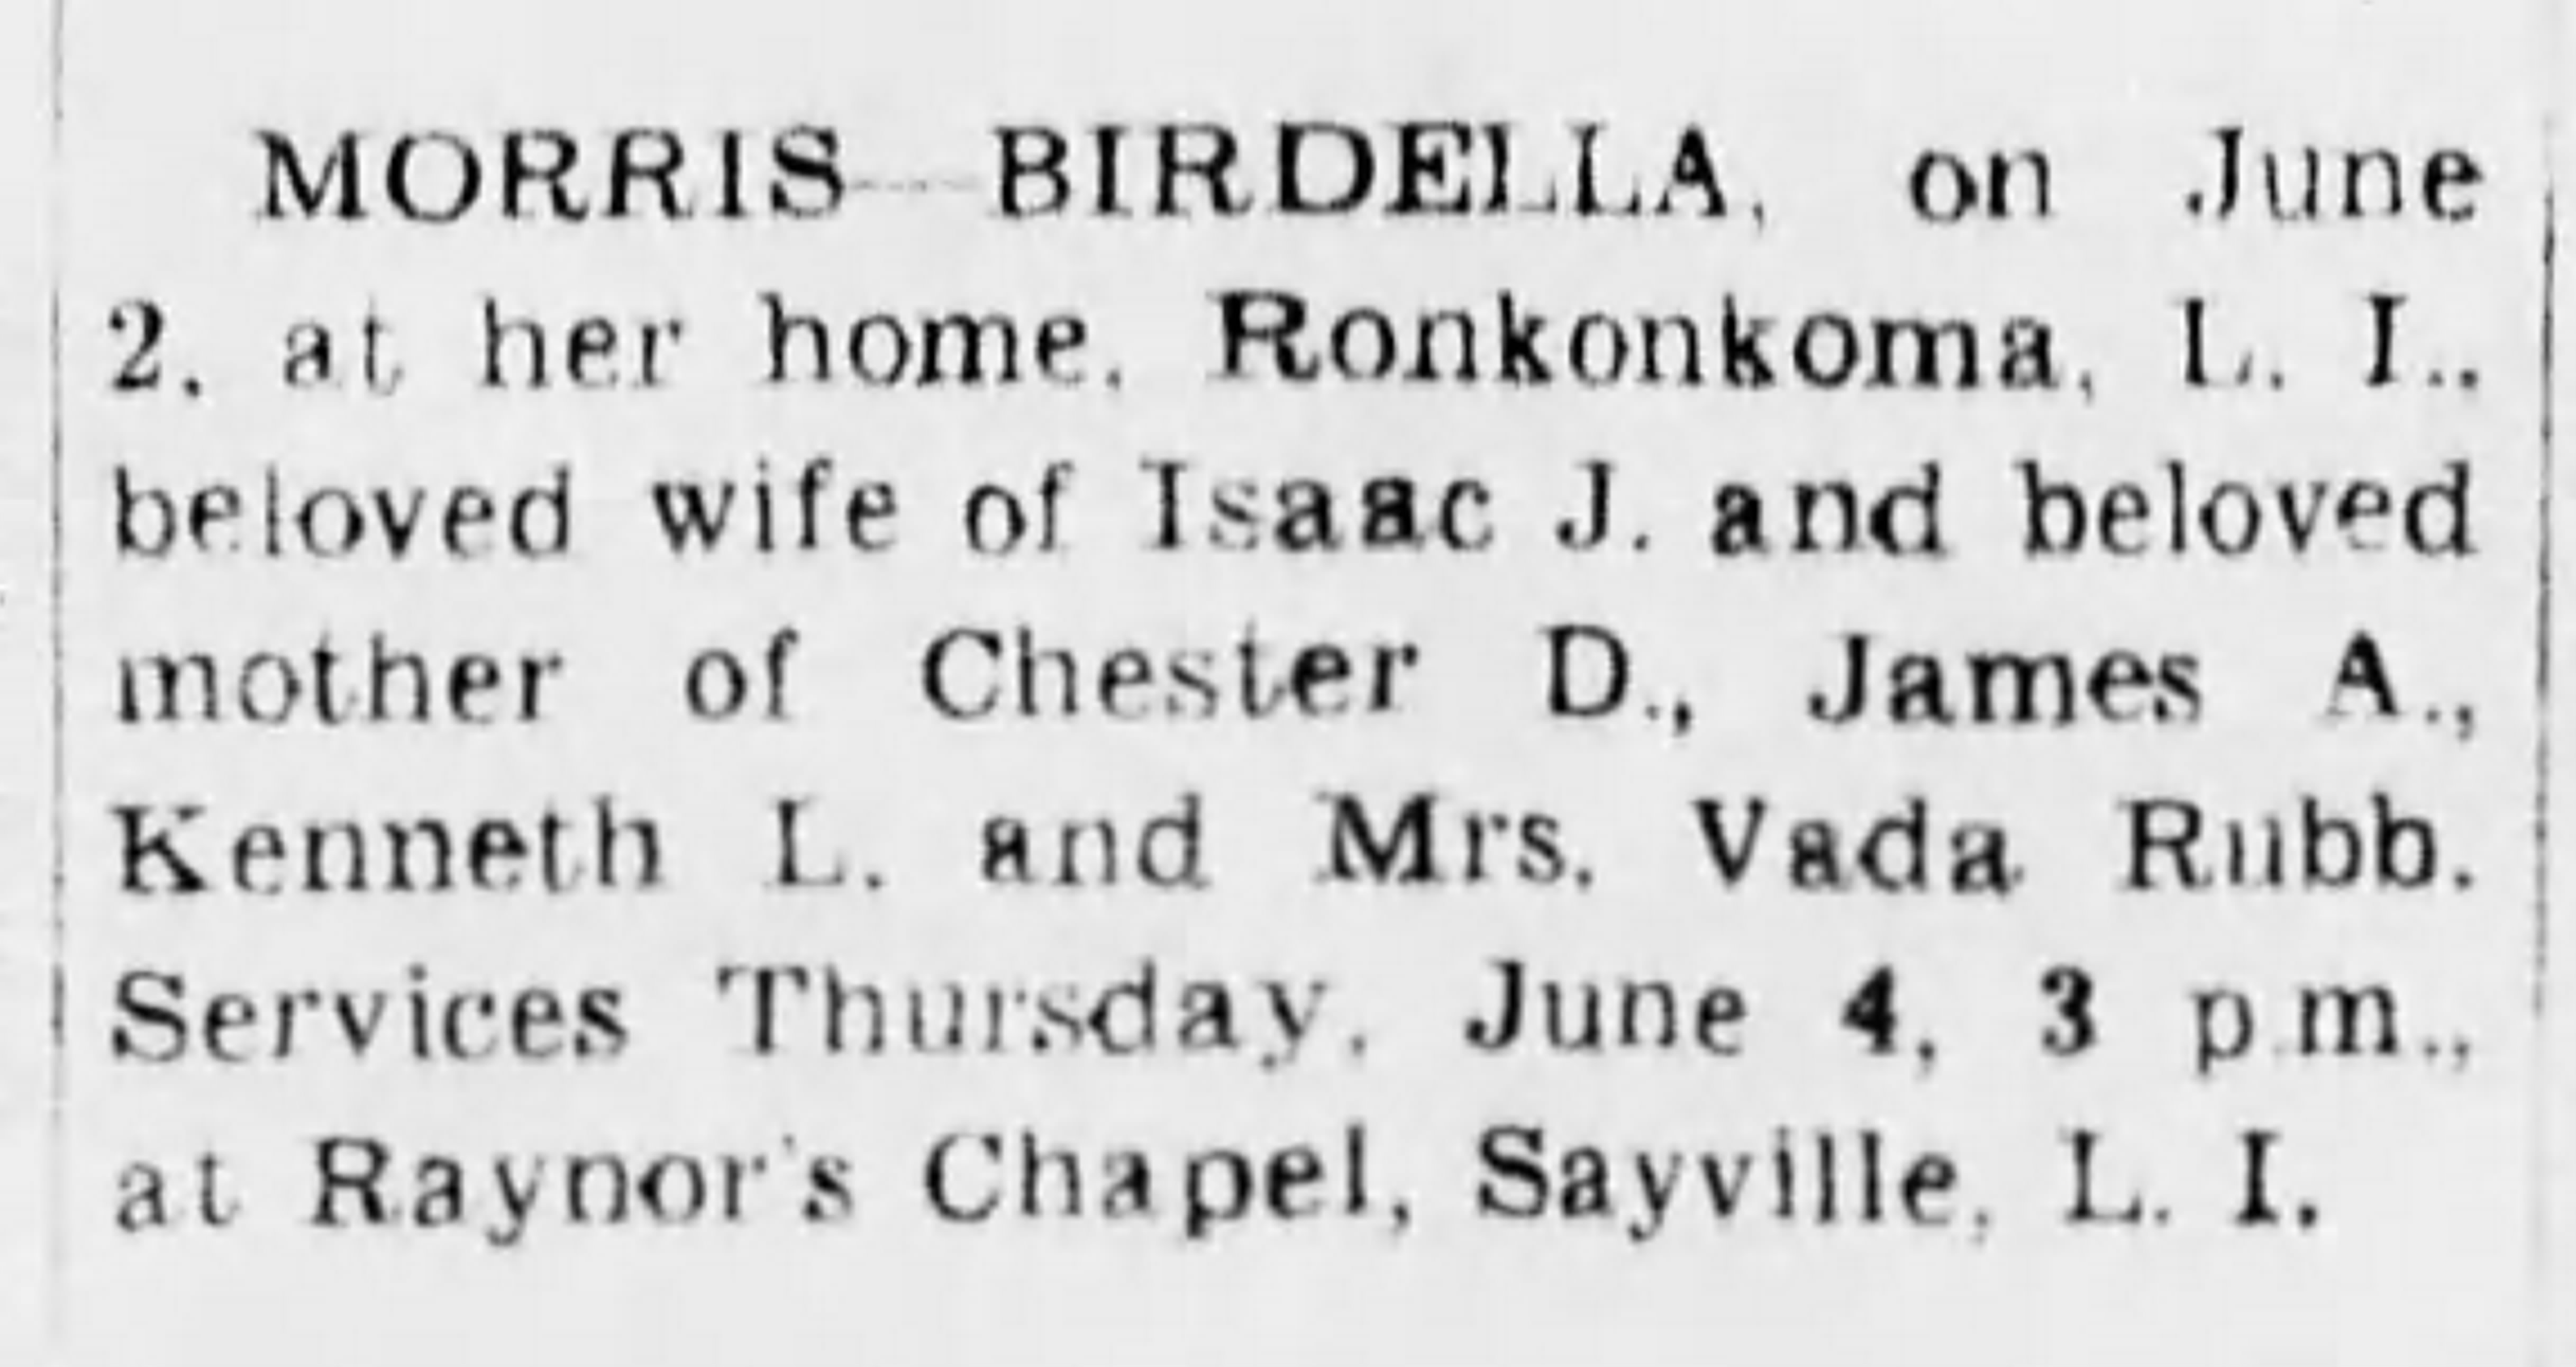
\includegraphics[scale=0.03]{images/The_Brooklyn_Daily_Eagle_Wed__Jun_3__1942_.jpg}
\caption{The obituary of Birdella L. Morris from the Brooklyn Daily Eagle, printed June 3, 1942, page 15. [Source: \url{http://bklyn.newspapers.com/image/52654292/}, accessed August 16, 2014]}
\end{figure}

When Pop had recovered, he told us what had happened. The previous night Pop, who was treasurer of the school about a hundred yards from his house, had been attended a meeting of the Board. While there, he received an incoherent phone call from Mom asking him to come home quickly. He ran home and found her on the floor in critical condition. She had suffered a heart attack but had managed to crawl to the phone to call Pop. It was the beginning of the end, for she survived for only a few hours. 

Mom was buried in an old but unused family plot inherited from Grandma Morris in Union Cemetery in Sayville\footnote{Union Cemetery is associated with Saint Ann's Episcopal Church in Sayville.}. Pop stayed on for a short time in the Ronkonkoma house and then moved in with Vada and Roy in their Sayville Home on Lakeland Avenue. It was fortunate for him during those trying days that Vada and Roy lived nearby, that Kenneth and Alice were next door and Aunt Carrie in the little cabin on the property. 

Later Pop sold the Ronkonkoma property on the North side of the railroad, Kenneth and Alice sold their home in the grove and brought one in Babylon. With these moves the old ``homestead'' was gone but not with it the memories of the happy family gatherings over the years. These memories will remain with us as long as we live. 

Back in Brooklyn, Mabel and I had long thought of moving to the suburbs where Jimmie would have the opportunity for more play room and more congenial playmates as well as better school facilities. We, too, wanted a one family house away from the encroaching apartment houses and crowded life of the city. We had been restrained form making such a move because of Dad's reluctance to leave Brooklyn. However, we felt that such a move must be made for Jimmie's sake. 

During 1942 or 1943 our search for the type of home we wanted took us to Jersey, Westchester and Long Island. Finally in December 1943, we noted an advertisement of a six year old house in \href{http://en.wikipedia.org/wiki/Rockville_Centre,_New_York}{Rockville Centre}. It was a cold Sunday with snow on the ground but the wording of the ad was appealing and we decided to drive out and look the house over. And we were happy we did, for it was the type of home we had been seeking for a long time. After the usual dickering on price, we signed a contract and, after a complete redecorating job, moved in the following March. 

Twenty years later, here at 60 Roxen Road on a hot August afternoon I am sitting on the back porch of that house writing these words and enjoying the tree shaded lawn and garden. In the interval since purchasing the home, as my income increased I have resisted the suggestions of friends to sell out and move to a more pretentious place> But Mabel and I liked it and it is very possible that it will remain our permanent home. 

At the time we moved, Rockville Centre was not as built up as it is now. Immediately behind our home was a large grove of trees and just to the east starting at a rear gate in our fence were several acres of cleared land that had once been a DeMott farm. Here we planted a victory garden adjoining similar vegetable gardens of our neighbors. And here too we became acquainted with our neighbors, who, like us, were helping the war effort by raising what we could of our own produce. Jimmie went to Hewlett School\footnote{The author is referring to Jennie E.~Hewitt Elementary School at 446 Hempstead Avenue, Rockville Centre, NY 11570} which was only four blocks away and later to South Side High School. We joined St.~Mark's Methodist Church and before long were well established in our new environment. 

In June, a neighbor and owner of Forest Lake Camp at \href{http://en.wikipedia.org/wiki/Lake_George_(New_York)}{Lake George} dropped in to inquire if we would be interested in giving Jimmy a month's vacation at his resort. Jimmy was enthusiastic and we gave our approval. At the beginning of July (or August) we packed him up with special camp clothing and equipment and drove him to \href{http://en.wikipedia.org/wiki/Grand_Central_Terminal}{Grand Central Station} where the boys were entraining for the camp. We found the waiting room jam-packed with boys and girls awaiting their trains to various summer camps. Shoving our way through the milling and noisy crowds we finally found the standard of Forest Lake Camp and a young counselor. Here we left Jimmy for his summer adventures. He evidently had a great time for he wanted to return in 1945. And he did. 

Shortly before his departure, I had a call from Dave Colville, a neighbor, whom I had not met. He wondered if I was planning to drive to Lake George and, if so, would I have room for him and his wife and son David who was going to the same camp as Jimmy. Despite the shortage of gasoline, I had managed to accumulate sufficient ration coupons and welcomed the company of the Colville family. After leaving the boys at the camp we put up at a little hotel at the lake and spent a very enjoyable weekend. 

Later, Mabel and I spent our two weeks vacation with the old ping pong crowd at a boarding house, Craig Hall, in \href{http://en.wikipedia.org/wiki/Great_Barrington,_Massachusetts}{Great Barrington, Massachusetts}. We had a glorious time with Bill and Effie Schweickert, Al and Gladys Platt, George and Georgiana Platt and Russell and Jane Lyman. The owners of the place, Alan and Mattie Craig, became fast friends. The good time was climaxed with the news on August 15 that Japan had surrendered. Germany had surrendered three months earlier and now the long and terrible war was over. We joined the happy throngs in the streets of Great Barrington and ended our celebration with champaign at Craig Hall. 

Jimmy had an active and enjoyable vacation, also. He competed in various sports and earned his award in swimming. The exertion he put into his qualifying tests in swimming, however, had a distressing and nearly fateful result. The day he returned from camp Mabel had prepared a steak dinner of the kind which he had previously so much enjoyed. He tried hard to show his appreciation but could not eat complaining that he did not feel well. We put him to bed, called in the doctor and received a terrible shock. Jimmy had contracted \href{http://en.wikipedia.org/wiki/Poliomyelitis}{polio}. 

Dr.~Burdick was very much concerned and informed us that his condition was serious. He reserved hospital facilities for a possible quick move if required and kept a careful watch on him through that long, long night. Jimmy and his mother and I went through a long period of anguish before we had hope that he would survive and would not be crippled. The experience, however, left him with one leg just a little shorter than the other, a condition which seems to have corrected itself through the years. During his convalescence, we kept his room piled with toys and games and did everything possible to ease that long period of inactivity for him. I am afraid we spoiled him a bit with our care. But we were very, very happy that he was on the way toward a normal life again. 

Meanwhile at the office, I was working hard and with the long hours which now seemed a normal work day. A few months after I had been transferred to the Corporation's Public Relations Department, it was suggested that I join the Shareholder Section of the Department. The activity involved the preparation and production of the GM annual and quarterly reports, special messages to shareholders and shareholder correspondence. In short, the job had to do with all staff work pertaining to our relations with shareholders with the exception of record keeping shareholders and shares which was the responsibility of the Stock Transfer Department -- a very large group compared with our little outfit of six or eight persons. 

I strongly resisted the suggestion. Such a move, I felt, would place me again in the type of work I thought was behind me. However, the pressure to make the move became so compelling thatI reluctantly agreed to take the job. If I had not, my progress would have been greatly retarded. One cannot buck the wishes of management and hope to survive in a progressive organization. In retrospect, the move was a good one for me. It placed me in a position where I could best utilize the talents which the management recognized I had, but which I diid not think were the kind that would lead to advancement. During my many previous assignments, I had developed a substantial sense of policy -- a qualification which was essential in the new job an was no doubt the reason for the assignment. In the long run, the job was rewarding -- both financially and in terms of personal satisfaction of accomplishment. 

It had been the practice of Board Chairman of the Corporation Alfred P.~Sloan, Jr., to write the annual and quarterly reports to shareholders and then send them to our section to put them in proper form along with appropriate illustrations for further check with the departments and executives concerned prior to final approval and publication. Our first problem was the editing of the rough hand-written copy Mr.~Sloan had prepared. I received a good introduction to this problem when I assisted in the 1941 annual report. Jack Dimond, who was Director of Shareholder Relations, was a meticulous, painstaking worker who scrutinized every word and phrase to make certain that Mr.~Sloan's intended meaning could not possibly be misinterpreted through our editing. This meant many long hours in poring over the copy, discussing the semantics and rewriting when necessary to do so. Oftentimes we would be at our desks until 2 or 3 am, then go to a nearby hotel, catch a few hours of sleep and return to the office by 8 am.

This seemed utterly time consuming to me and a situation that should be corrected. When the time approached for beginning work on the 1943 report, I recommended that we assemble the facts on the operations for the year, have a talk with Mr.~Sloan on the approach he would prefer and then write the report ourselves for his approval. The recommendation was accepted. We wrote the copy, adopted a new format in a more readable size and with more illustrations. Mr.~Sloan was happy with the result and requested that we continue a like practice on future reports. Although the job was still a tough one, we had relieved ourselves of a heavy burden.

Possibly as a result of the acclaim accorded the 1943 report, and the further improved 1944 report, within the Corporation and by shareholders, I was appointed Director of Shareholder Relations in the Fall of 1944, a job I held until my retirement in 1957. Jack was made head of the Editorial Section in Detroit. Throughout this period of change for me, the nation was in a war economy and General Motors was exerting an all-out effort in producing war materials. It was a most abnormal period of manpower and material shortages. \href{http://en.wikipedia.org/wiki/William_S._Knudsen}{William S.~Knudsen}, GM's Danish born President, felt that he owed his success to the land of his adoption and had accepted the Government's request to head the nations war production. My old boss, James D.~Mooney, who was Vice President of Overseas Operations had left to join the Navy and many other top executives were wither serving in Washington or in the armed forces. In the office departmental lines were broken and all were pitching in cooperatively to get the work out. 

Mr.~Garrett continued to call on me on special assignments similar to those in my former job. I made presentations to the Public Relations Policy Group which was headed by Mr.~Garrett and included the President and top officials of the Corporation. I also continued to assist in the development and analysis of Public Opinion surveys through the facilities of the Opinion Research Council and the \href{http://en.wikipedia.org/wiki/Harcourt_Assessment#The_Psychological_Corporation_.281921.29}{Psychological Corporation}. The association I enjoyed with Dr.~Claude Robinson, President of Opinion Research and Dr.~Henry Link, President of Psychological helped me keep my finger on the pulse of public opinion -- a factor which was a good advantage in my writings for Mr.~Sloan and other executives during a troublesome period when public attitudes were changing rapidly. 

All business now was acutely aware of the new social thinking on the part of the public. An awareness that had been slowly awakening with the development of the \href{http://en.wikipedia.org/wiki/New_Deal}{New Deal} programs since the first election of \href{http://en.wikipedia.org/wiki/Franklin_D._Roosevelt}{Franklin D.~Roosevelt} in 1932. The election of Roosevelt to a third term in 1940 and to a fourth term in 1944 together with the impact of the war had intensified this mounting public social consciousness. Business had to keep abreast of the resulting rapidly changing attitudes with regard to the economy and to business itself. Our use of public opinion surveys became a useful tool in helping us do so.

One manifestation of this new thinking, as it applied to my own work, was an increased awareness on the part of the stockholders that they were in fact the owners of the business and should be concerned with the management and progress of their corporation. This concern or interest was heightened by the emergence of the so-called independent stockholders who attended annual meetings of various companies and expressed their views. Sometimes they expressed approval of the management's actions, but more often spoke in opposition. A few were wealthy and held stock in many companies. This gave them many opportunities to share the spotlight with management and to obtain publicity for themselves. Others represented groups or associations of stockholders, some organized to harass management, it seemed, and others to support management.

The Corporation's may have been at fault in opening the door to larger attendances at their meetings through making available larger facilities and serving lunches to shareholders. General Motors was no exception. Until 1947, it had held its meetings in an office in the \href{http://en.wikipedia.org/wiki/DuPont_Building}{DuPont Building in Wilmington}. I attended one or two of these meetings as an observer. Aside from the necessary officers to legally run the meeting only two or three other stockholders were present. However, with the opening of a \href{http://en.wikipedia.org/wiki/Wilmington_Assembly}{B.O.P.\footnote{B.O.P. refers to manufacturing products for Buick, Oldsmobile, and Pontiac.} assembly plant} just outside of Wilmington, its large cafeteria was made available for our meetings. Luncheons were served, the popularity of the meetings increased, the independent stockholders had a larger sounding board and with the addition of tents to care for the overflow crowds, the meetings took on the atmosphere of a circus. 

All this meant more responsibility and more headaches for my department. First of all, there was the need to have someone attend annual meetings of the other companies and report back to me the activities of the vocal stockholders so we could in turn inform the management on what kind of questions would be asked at our meeting. In addition, we had the task of replying to all inquiries received with proxies, of arranging for the meeting and the lunch and for the executive dinner on the eve of the meeting in Wilmington, the greeting of shareholders in the lobby of the plant on the day of the meeting and the preparation of the post-meeting report to stockholders. As the stockholder family increased, the responsibility likewise increased.

The executive dinner mentioned was held in the DuPont Hotel. In attendance were the Chairman, President, Secretary and other interested officials and staff members. Here we would have last minute discussions of the arrangements for the meeting and tie together any loose ends that might be uncovered. A welcome respite after the hectic activity of the pre-meeting and meeting projects was the ride home in a special railroad parlor car where we relaxed with refreshments and good fellowship. There was only one more bridge to cross on the overall project. That was the post meeting report which in later years we started writing on the homeward bound train.

There were so many interesting incidents and many difficult ones too that we would like to relate, but if we pause too long on them, I am afraid we will not be able to finish our story. So we will have to go on and backtrack where necessary. 

\begin{center}
------------------------------------------------------
\end{center}

One of the special jobs assigned to me during the war was the writing of Mr.~Sloan's Christmas messages to General Motors executives. Three of them uncovered in an old file reflect my attempts to express optimism and, at the same time, gird the organization for further effort during this unforgettable period in world history. Here are some excerpts, from the December 25, 1943 message:

\begin{quote}
Once more my message of Christmas greeting is sent to you in wartime. The dramatic events of the year have brought into clearer focus the prospect for peace. In the fighting fronts of the world, the direction of battle is slowly but surely turning toward victory for the United Nations. On the home front, underlying all other issues, there is a unity of purpose and effort in support of the fighting forces, with a resulting ever-increasing flow of the weapons of war and the essentials for the men who need them.

In face of terrible sacrifices of human life and human values, it is difficult to express the greetings of cheer customarily extended at this season. We can be sincerely thankful, however for the turning of the tide of battle. We should be thankful also for the part that the General Motors organization has been privileged to play in the overall effort of the nation. With the task of conversion to war largely completed in 1942, the General Motors Organization during the year now closing had the opportunity for the first time to concentrate its experience and skills on the job of production itself... The sum of the individual efforts is an overall contribution of which we can all be proud. 
\end{quote}

And here are some excerpts from the December 1944 message: 

\begin{quote}
At this holiday time, far deeper that the war and its untold sufferings, there lies in the hearts and minds of the people throughout the world the imperishable spirit of the season -- Peace on Earth. Good Will Toward Men. While peace may be denied for us for 1944, the prospect for peace is brighter than it has been since the outbreak of war. There is still much to be done before the war is won, but there is no doubt as to the ultimate result. Thanks to the initiative and courage of our fighting men, victory is inevitable.

With victory will come a new challenge and a new opportunity for us all -- a challenge to help restore our country to its peacetime pursuits, and an opportunity to go forward to greater accomplishments in the postwar world to follow.

It must be a source of gratitude to you, as it is to me, that we in General Motors have had the privilege of contributing to the overall effort of American industry in support of our fighting men. The magnitude and character of the contribution 1944 constitute a record in which we can all take pride. It reflects the experience, planning, resourcefulness and teamwork of an alert and vigorous organization, and I want to congratulate each of you for your part in it. The effectiveness with which we apply these elements of accomplishment in meeting the challenge... peacetime production... will be a measure of General Motors' contribution to the winning of the peace.
\end{quote}

With the end of the war in August 1945 and the resumption of civilian production to meet the pent-up demand for cars and trucks, General Motors was faced with another crisis. This was the \href{http://en.wikipedia.org/wiki/United_Auto_Workers_(UAW)_strike_of_1945-46}{strike by the UAW on November 21, 1945}. As a result, production was again halted and practically no vehicles were produced until the second quarter of 1946. The Corporation had embarked on an extensive postwar program of modernization and expansion and hoped to capitalize on a marked starved for vehicles following a four year period of shortages.

My section, along with other sections of the Public Relations Department, was called upon to pitch in and help publicize General Motors case in an effort to win public support. It was another period of pressures to meet deadlines and is cited merely to indicate the futility of anticipating smooth sailing in business at any time. Forces over which management has no control cannot always be anticipated. Their impact is unpredictable. In my relatively brief business career up to this time, business had felt the impact of two world wars, one great and several smaller depressions as well as disturbances arising from the increasing pressures of a world-wide social revolution (often politically motivated) of which labor unrest was a significant part. In addition there was the growth of conflicting ideologies of government with the spread of communism. Despite all such retarding factors, the longtime trend of business was upward. The population was expanding and markets widening. A rapid advancement in science and technology was resulting in better ways and means of making more and better things for more people. 

A review of the longtime trends of tGeneral Motors business bears this out. There were the temporary impacts of unfavorable national and international factors, but following each there was a decided upward trend. To those involved at the time, however, the depression factors seemed more permanent than temporary and resulted in personal pessimistic views of the future and of ones own ability to bear up under the strain.

My responsibilities in stockholder relations opened up many new opportunities for widening my contacts with General Motors management and supervisory personnel in New York and Detroit and with executives of other companies concerned with stockholder relations. In the latter part of 1946 or the early months of 1947, a chap named Bruce Watson from the \href{http://en.wikipedia.org/wiki/General_Foods}{General Foods Corporation} called at the office to discuss our methods and techniques in the stockholder area. Recently discharged from military service, he had been hired by General Foods to set up a specialized department in that area. A few weeks later Emery Cleaves, a vice president of the Celanese Corporation, engaged in a similar project dropped in for a discussion of the subject. Later, we had frequent luncheon meetings to which we invited Harry Green of \href{http://en.wikipedia.org/wiki/Johns_Manville}{Johns-Mansville} and Henry G.~Martin Secretary of \href{http://en.wikipedia.org/wiki/Standard_oil}{Standard Oil}.

The five of us were concerned with the need for a broader two-way understanding between management and stockholders on mutual problems and a deeper awareness by both of the wide areas of common interest. We recognized that stockholders had become increasingly aware of the fact that they were the owners of the business and as such were entitled to have presented to them all the facts of the business. Our managements, particularly that of General Motors, had followed the practice of full reporting for many years but some others had not and we felt that all managements might be penalized because of the shortcomings of a few. Industry had been the ``whipping boy'' of the New Deal and management badly needed full stockholder support. In light of these circumstances, we felt that an organized medium for the exchange of information concerning policies and practices affecting corporate stockholder relations would be constructive. It would also encourage adherence to high ethical and technical standards in the practice of stockholder relations. 

On September 24, 1947, we formalized this thinking with the organization of the Stockholder Relations Society of New York. The first meeting was held on that date at the Harvard Club with the objectives set down along the lines described above. In addition to the five founding members, the charter members included representatives from \href{http://en.wikipedia.org/wiki/Sylvania_Electric_Products}{Sylvian Electric Products}, \href{http://en.wikipedia.org/wiki/Consolidated_Edison}{Consolidated Edison}\footnote{Commonly referred to today as Con Edison or Con Ed.}, \href{http://en.wikipedia.org/wiki/Union_Camp_Corporation#Union_Bag_and_Paper_Company}{Union Bag \& Paper}, Lone Star Cement, \href{http://en.wikipedia.org/wiki/Curtiss-Wright}{Curtiss Wright}, Borden and Eastern Gas and Fuel. Other members admitted later included representatives of \href{http://en.wikipedia.org/wiki/Allied_Corporation}{Allied Chemical}, \href{http://en.wikipedia.org/wiki/Union_Carbide}{Union Carbide}, \href{http://en.wikipedia.org/wiki/Merck_\%26_Co.}{Merck \& Company}, \href{http://en.wikipedia.org/wiki/Kennecott_Utah_Copper}{Kennecott Copper}, \href{http://en.wikipedia.org/wiki/U.S._Steel}{United States Steel}, \href{http://en.wikipedia.org/wiki/AT\%26T}{AT\&T}, \href{http://en.wikipedia.org/wiki/United_airlines}{United Airlines}, \href{http://en.wikipedia.org/wiki/General_electric}{General Electric}, \href{http://en.wikipedia.org/wiki/National_Lead}{National Lead}, \href{http://en.wikipedia.org/wiki/IBM}{IBM}, \href{http://en.wikipedia.org/wiki/DuPont}{DuPont}, \href{http://en.wikipedia.org/wiki/Raytheon}{Raytheon}, Hercules Power, and \href{http://en.wikipedia.org/wiki/CBS}{Columbia Broadcasting System}\footnote{Known today as CBS.}. Some of the companies mentioned were added after my retirement, but we did have a very representative list of big business executives during my 10 years of active participation in the Society. 

An unwritten rule of the organization did not permit publicity on the meeting discussions. As a result members felt free to ``let their hair down'' and talk freely. I believe that the Society, particularly in its early years when the need for it was the greatest, did much to raise the standards of management-stockholder relations and to indirectly improve the public image of industry. It was helpful to me in widening my contacts with people who practiced my profession. Many of them were officials of their corporations. One during my tenancy as president was \href{http://en.wikipedia.org/wiki/Lammot_du_Pont_Copeland}{Lammot du Pont Copeland} who was vice president of DuPont and now its president. These contacts gave me, as they gave to other members, an open door to the experiences of many companies in building better management-stockholder relations. As of this writing, the Society is still very active and still doing the constructive job it was designed to do by its founders 18 years ago.

General Motors had always been a little ahead of the majority of companies in its dealings with shareholders. Through the years, Mr.~Sloan had followed the practice of full reporting of the pertinent facts of the business. As a matter of fact, he included in each annual report a statement ``Policy of Giving the Facts'', a statement which was repeated for several years after we had modernized and streamlined the annual report in 1943. That face-lifting effort was designed to make the report more attractive and appeal to the recipient to open it and read it. In the 1948 report we went further by the addition of color pictures and charts and a cover painting by a well-known artist. In the planning for this move, we had secured the approval of management for cover color paintings suggestive of the place of the automobile in the American way of life. These paintings of typical American scenes were done by such artists as \href{http://en.wikipedia.org/wiki/Stevan_Dohanos}{Stevan Dohanos}, \href{http://en.wikipedia.org/wiki/John_Falter}{John Falter} and Melbourne Brindle. We think they appealed to the stockholder and stimulated an urge to open the report and read it. 

For several years, starting with the 1944 report, we had won the Financial World's award for the best report of the automobile industry, but the proof that our continued efforts to improve the report was successful came in 1950 when the 1949 report was voted the best in the industry. The Award dinners were annual events held at one of the local hotels and attended by executives of practically all important corporations in the New York area and from many outside of New York. My assistant, Bill Trenn, and I would arrange for a suite of rooms with facilities for serving beverages and snacks to our business friends before and after the dinner and formal presentations. This gave us additional opportunities for renewing old contacts and making new ones. 

Another such event was the annual Financial Follies show put on by the financial writers of the New York newspapers. This was a more pretentious affair attended by Corporation officials. Here Paul Garrett would set up a large suite with bar and his section heads would serve as hosts to visitors. I had the opportunity to meet top officials of many large corporations at these affairs.

Being a part of Public Relations meant that one was called upon to many affairs. In the fall of the year at New Model Announcement time, there was Mr.~Garrett's party for the press at the University Club, the Preview of New models at the \href{http://en.wikipedia.org/wiki/Waldorf_Astoria_New_York}{Waldorf} for invited guests and the special hosting facilities set up by our Press Section in a suite at the Waldorf. During those years, the new models were shown at the Waldorf, the wind-up affair was a party for public relations personnel, for the whole department which had carried a heavy burden of work before and during the show. 

The pace of the job was fast and little time was left for the family during the forties and early fifties. I sometimes wonder if it was all so necessary, if I could have handled my job a little easier than I did. But the ``nature of the beast'' is the determining factor and it is difficult to change one's methods. 

During this period Mabel and I both lost our fathers. My father died on October 30, 1947 at the age of 79 years and 8 months. He had been ailing for some time and had become quite senile. He was laid to rest alongside Mom in Union Cemetery. Mabel's father passed away on April 1, 1951 at the age of 84 and nine months. He was hale and hearty until a month before when he had fallen down our front stairway on Roxen Road. He did not recover from the shock. He was buried with Mother Norseen in \href{http://en.wikipedia.org/wiki/Cemetery_of_the_Evergreens}{Evergreen Cemetery} in Brooklyn. Dad was survived by the youngest of his brothers, the Reverend Oscar Norseen, who, at this writing, is nearing 90 years of age and living at Covenant Palms, a retirement home for Swedish church members in Miami, Florida. Two other brothers, Henry and David, a sister, Emma Johnson, had died some years ago. At Pop's funeral, I saw Aunt Carrie (Mom's sister) for the last time. Since leaving Ronkonkoma, she had been living with her son (Fred Mather) in New Brunswick, New Jersey. We do not know what happened after that.

\begin{figure}
\centering
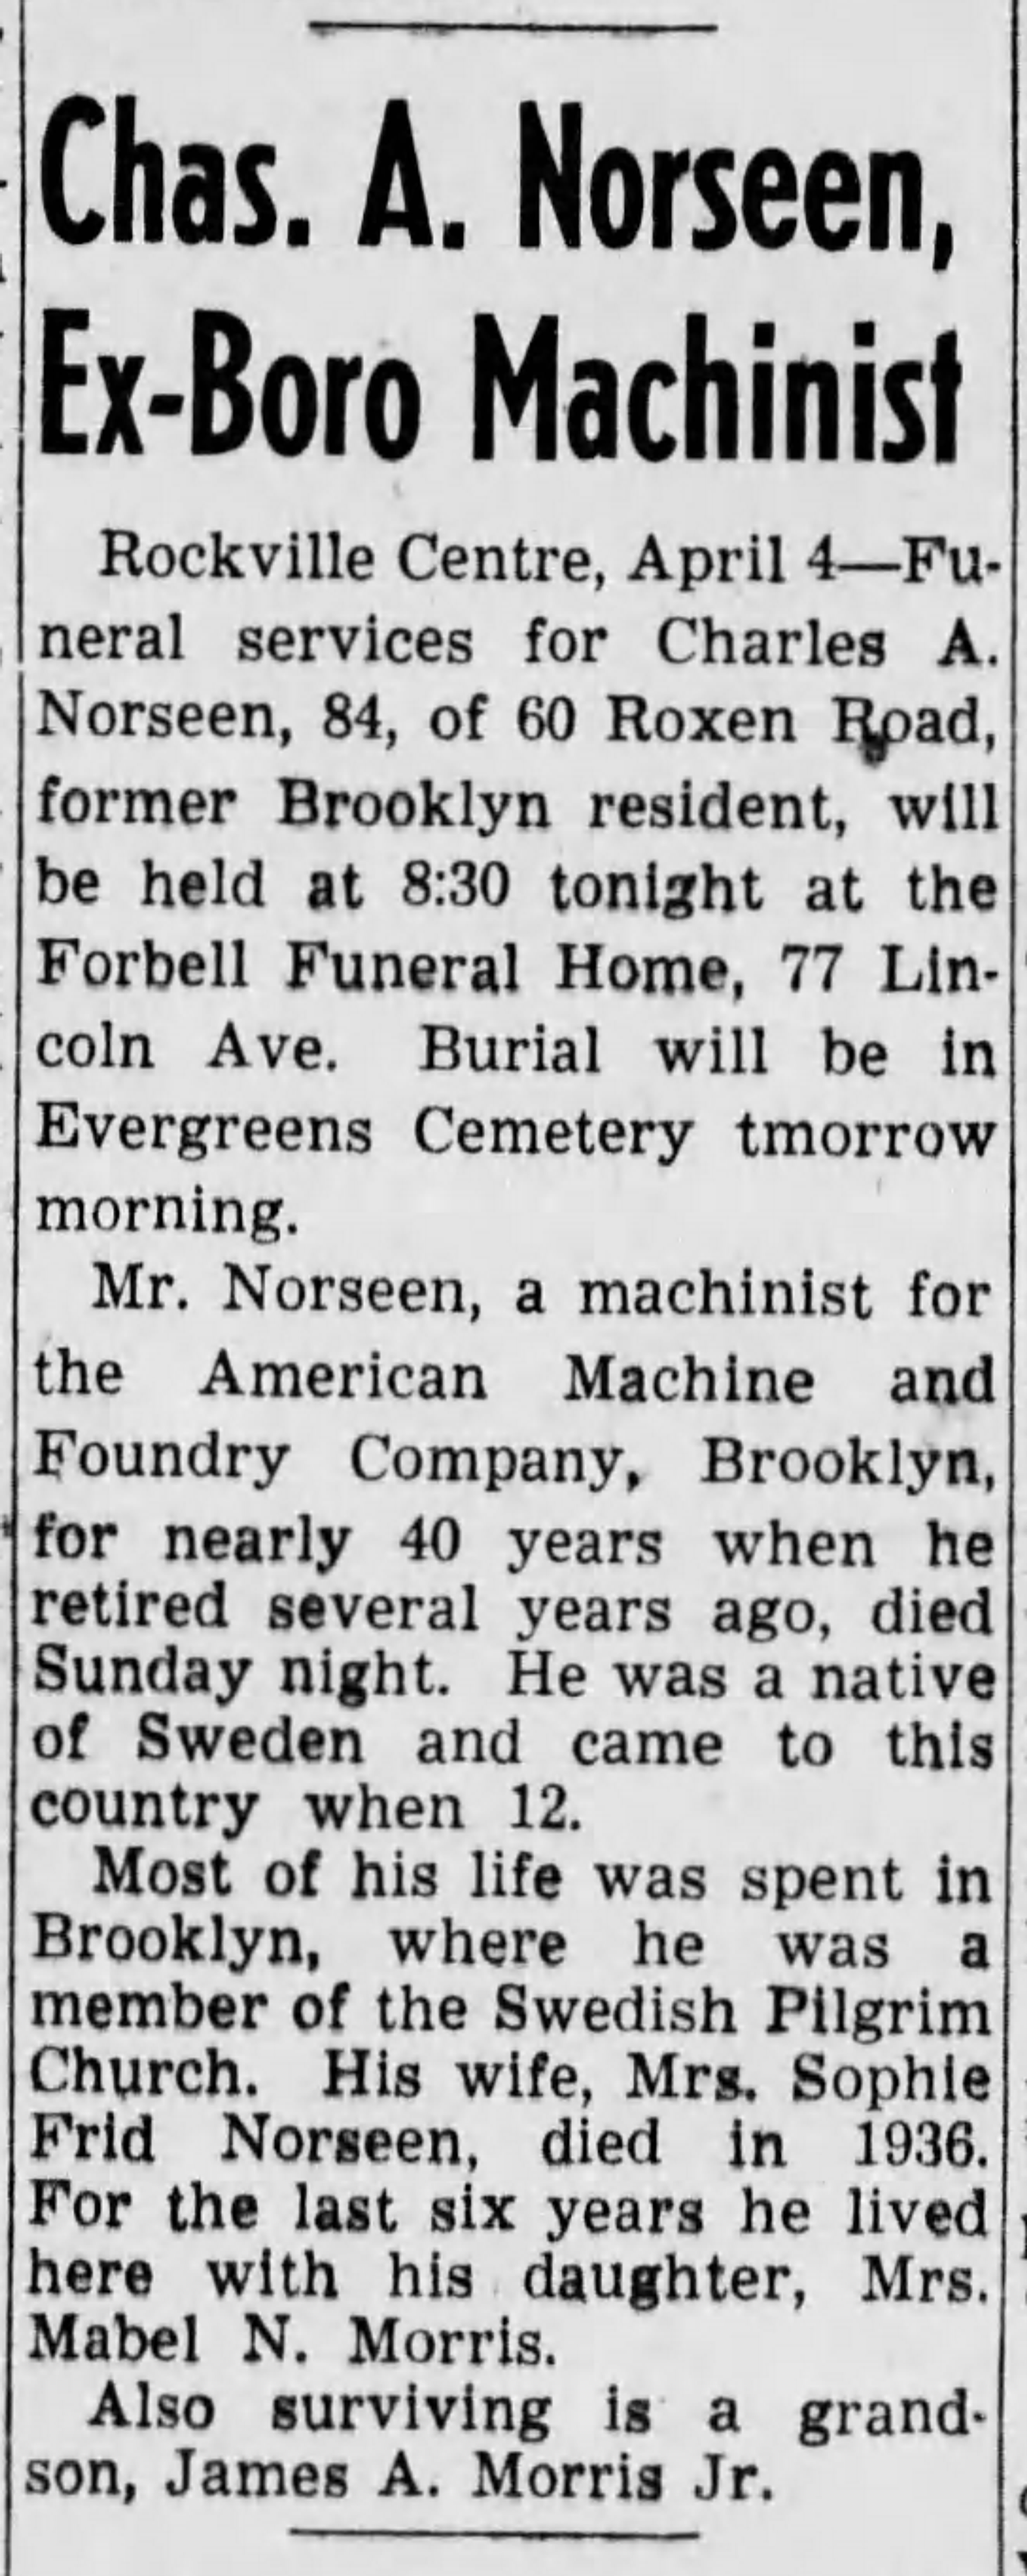
\includegraphics[scale=0.03]{images/The_Brooklyn_Daily_Eagle_Wed__Apr_4__1951_.jpg}
\caption{The obituary of Charles Norseen in the Brooklyn Daily Eagle, printed April 4, 1951, page 15. [Source: \url{http://bklyn.newspapers.com/image/52644213/}, accessed August, 2014]}
\end{figure}

The passing of our fathers marked the end of the old order. We were now the ``elders''. Marriages and births were expanding the ``juniors''. As mentioned previously, my niece Evelyn had married Robert Veritzen in 1938 and now had a son, Donald, born in 1946. After returning from the war, my nephew Roger had married Ceil Weisse in 1944 and in 1946 were blessed with a daughter, Susan, and in 1949 with a second daughter, Karen. My niece, Miriam, had married Andrew Rothhaupt, also a war veteran, in 1944. In 1946 their son Terry was born followed in 1950 by a daughter, Alice-Lynne. My nephew, Donald Rubb, married Sally Reynolds in 1952 and their first son Alan was born the same year. 

Jim was growing up. He had gone through Hewlett School and on to Junior and Senior High School from which he was graduated in June 1951. The high school years are the tough ones for the parents. I say this because the child is maturing, he wants to assert himself and free himself, in a sense, from the restraints of his parents yet he recognizes his dependency on them. For a time, it is difficult to keep open the lines of communication. The parents wonder if they are handling the situation correctly and the child wonders if they were ever young themselves and understand the thinking of the younger ones. This is somewhat of a generalization as Jim was no different from any other boy of his age. At school he was an average student. He was interested in sports, a member of the Glee Club and other high school societies. He also took piano lessons for a short time and then switched to applied harmony. 

Maybe we had had such a tough fight to raise ourselves by our bootstraps, we may have been a little more indulgent than we might have otherwise been. I know that Jim lacked nothing. When he had reached ``driver permit'' age of 17 in July 1950, we bought him a Chevrolet Coupe. Because of the privelege granted by GM, I was able to get cars at a discount and for a couple of hundred dollars each year could buy him a new one. He drove new models in 1951, '52 and '53. When he graduated from College, we presented him with a Buick. Jim spent several summers with us on my vacations in \href{http://en.wikipedia.org/wiki/Sebasco_Harbor_Resort}{Sebasco} in Maine. 

In the fall of 1950 or the spring of 1951, Jimmie had applied for admission to \href{http://en.wikipedia.org/wiki/Cornell_university}{Cornell} and \href{http://en.wikipedia.org/wiki/Lehigh_University}{Lehigh} Universities and was accepted at both. To help him in his decision as to which he would prefer, we took him on a tour of inspection, first to Ithaca and then to Bethlehem. He was very much impressed with Cornell. It was on a beautiful campus but its size was a bit frightening and he chose Lehigh where he thought that because of its smaller enrollment, he would have a better opportunity for getting into more activities and for making friends. His choice was not one of snap judgement. I recall that he was uncertain during our drive home. After further discussion at dinner, I suggested that he take a walk alone and think hard. He returned to the house a half hour later with his mind made up. He had selected Lehigh. 

In September of 1951, we packed his luggage into our car and drove him to Lehigh where we helped him locate in his dormitory. A year later, he became a member of the \href{http://en.wikipedia.org/wiki/Kappa_Alpha_Society}{Kappa Alpha Society} and resided in the fraternity house for the rest of his stay at Lehigh. Mabel and I spent many enjoyable visits with Jim and his friends at the fraternity house when we had come to Lehigh for football games or Parent's Day. 

Because of his proficiency in mathematics in high school, Jim had decided to major in engineering. Unfortunately, he could not measure up to the requirements and in a year or two switched to business administration. As in high school, Jim was an average student at college. At times it seemed as though he could not achieve passing marks in some subjects. Then, we would receive a warning from the Dean and Jim would plug a little harder. One summer he had to remain for special studies to catch up on his marks. But in the long run when he applied himself, he could squeeze through. Meanwhile, I kept a series of inspirational letters flowing to him, which I like to think were helpful to him in keeping his mind on his work. I knew he had the stuff, but during that period was lacking in initiative. 

It seemed that Mabel and I were always busy. She with her housework, her sewing, her church and club work, and I with my always present office homework, my gardening and housework. On the social side, we were also kept busy. Our ping pong club was now a card club meeting monthly at the homes of the Platts in Brooklyn, the Schweickerts in Maplewood, the Craigs in Forest Hills or at our home in Rockville Centre. The order of things were dinner at 6 pm on a Saturday evening and cards until midnight, then the long ride home. We were also members of the Couples Club of St.~Mark's which met one night a month in the church parlor with a committee appointed to provide the entertainment and refreshments, I had the chore (or pleasure) of writing plays for a number of committees on which I served. 

In addition there were the family get-togethers at Kenneth's or our homes and sometimes at Roger Morris's home after his move to Glen Cove. We did continue to have good times with our old friends the Hales and Smiths. We could not mention their names without the thought of good times. Wad and Marthe in the 1940s were living in a large house in Summit where we visited them often on weekends or at special parties. Merle's Salaried Personnel Activity had been headquartered in Detroit and he and Teddy were there again living in an apartment hotel. When they visited New York, the six of us would get together for dinner in New York or at one of our homes. More often, Merle would come in alone and we would have stag dinners together at his club.

In 1946 or 1947, Merle bought an old farm house in Bristol Hills near \href{http://en.wikipedia.org/wiki/Naples,_New_York}{Naples, New York}. It was in a beautiful section of the country which they liked so much that they bought two adjoining farms and still later additional purchases brought their holdings to a thousand acres, three farmhouses and a caretaker's house.

Merle and Teddy then went to work on a project that was probably the most enjoyable one of their lives, the remodeling of one of the houses and the building of a guest house. Merle, who was a graduate electrical engineer but never worked at it, had an opportunity to put some of his ideas into practice. The old porch of the farm house was enclosed, a new kitchen installed and a sun room added. This was followed by the reconstruction of an old barn into a combination garage, work shop and upstairs a guest house. The main house and guest house were connected with a large stone-walled patio including huge fireplaces and warming ovens for the outdoor cookouts at which Merle was a past master. Everything was electrical. The floor of the patio was radiant heated beds recessed in the four corners of the huge guest rooms moved out with the push of a button, there was a small kitchenette in the room with electric stove and refrigerator, and from a master panel varied color lights could be turned on to illuminate the patio. And all of this overlooked the rolling pasture land and wooded mountainsides of his own little world. Here we spent many happy days with the Hales and the Smiths.

Mabel and I would visit the ``Hale House'' direct from our vacation in Maine. The Smiths would usually drive up at the same time. And they, too, built their dream house on 14 acres of rolling country outside of Morristown, New Jersey. A beautiful house on a landscaped plot on the hill overlooking a valley with the mountains in the distance. Here, Wad built a stone guest house, or rather a combination library, office and print shop, where he worked on his Sherlock Holmes writings and printed a monthly magazine -- The Baker Street Journal -- for members of the Sherlockians of which he was the leader. He was probably the outstanding authority on the writings of Dr.~Watson (\href{http://en.wikipedia.org/wiki/Arthur_Conan_Doyle}{A. Conan Doyle}'s). The private road leading to the house was named Baker Street and the number on the cottage 221B, which was the address of Sherlock Holmes.

Wad and Merle could not understand why Mabel and I did not move from our home in Rockville Centre to some place in the country where we could have isolation on our land. We simply did not like that kind of life and much preferred to suburban home we had and the kind of life we were living. We liked to visit such homes as theirs but could not see them as permanent homes. I could not argue that my job was such as to permit little time for country life because their responsibilities were greater than my own and they were like me ``slaves to their work''. (I should add here that Merle's country place was a summer home only until his retirement in 1956. During most of the time he would commute to Naples for the weekends and for his vacation.)

Since taking over the stockholder relations job, I had had to make more frequent trips to Detroit to check with C.E.~Wilson, the President, and other executives and officials the copy we were preparing for various reports. Our procedure of checking included first of all clearance from New York officials, then checking with the vice president in charge of the legal staff, the vice president in charge of distribution, the executive vice presidents concerned and finally the president. Incidentally, before checking with these officials, we had to have the approval of their staffs. So, it can be seen that a tremendous lot of contacts had to be made. Usually while on these duties in Detroit, I attended meetings of the Public Relations Planning Committee of which I was a member. In addition two or three times a year there would be a Public Relations Regional managers meeting, and dinner in the evening, which I attended.

Mr.~\href{http://en.wikipedia.org/wiki/Harlow_Curtice}{Harlow H. Curtice} was made Executive Vice President in charge of the staff in 1948. He had been general manager of Buick and was a strong believer in the centralization of all staff activities in Detroit. Before he took over the presidency in 1953 he had tried to get many of us to move to Detroit and set up our headquarters there, I did not want to do this. But after he became president, the pressure became acute. The alternative was to set up an office in Detroit and be there two or three days each week. This I did. I was given a suite of offices, an assistant and a secretary. I would leave my New York office on the Detroiter on a Monday night, arrive in Detroit on Tuesday morning, check in at the \href{http://en.wikipedia.org/wiki/Westin_Book_Cadillac_Hotel}{Book Cadillac Hotel} and then go to my office. I would depart from Detroit on a Thursday evening, arriving in New York on Friday morning for a days work at my office there where I had my long-time personnel with Bill Trenn in charge. With Dad gone and Jim at college, this arrangement left Mabel alone for three nights a week. It was not a good arrangement. But for both of us it was far better than pulling up our roots in the east for the few years remaining of my business life.

Sometimes I would get a ride in either direction on one of the Company planes with Mr.~Curtice, Mr.~Donner, Mr.~Garrett or some other executive entitled to use them. Incidentally, Paul Garrett was also in the same predicament as I was. He had also set up an office in Detroit while keeping his residence in New York. He, however, had only one day a week in his New York office. That was on Fridays. While I usually put up at the hotel in Detroit, I would take a room in the executive suite in the GM building if I had late evening appointments with Mr.~Wilson or Mr.~Curtice. In this connection I would like to explode the myth that top executives of large corporations live ``the life of Riley''. From my own longtime personal observations, they work harder and put in longer hours than do their subordinates. Many times I would have appointments with the president, Mr.~Wilson before 1953 or Mr.~Curtice after 1953 at 6 or 7 o'clock in the evening or at 8 or 8:30 in the morning and then discuss a message with them for an hour or two. At other times, after a long evening of work with my associates, we would go to see the Recess Club in the adjoining Fisher Building for a late dinner at say 10 pm and find Mr.~Wilson or Mr.~Curtice just coming in for their dinner.

At luncheons in the executive dining rooms in Detroit or New York, we would see them closeted with other officials discussing business in the private rooms reserved for their use. Mr.~Donner, now chairman of the Board of Chief Executive Officers would take two or three jam-packed brief cases home over a weekend and return on Monday mornings with every memo marked and ready for distribution. It would be impossible for the average individual to handle the quantity of work that they did.

And each one had their own way of coming to a decision. On an interpretation of practice or policy in the copy submitted for their approval, Mr.~Wilson would swing around in his chair and gaze out the window for what seemed like an eternity and I would wonder if I should get up and leave. Then we would swing back to his desk with a suggestion as to the approach. Mr.~Curtice, on the other hand, always had a quick and positive answer. Mr.~Wilson was an engineer and Mr.~Curtice a salesman which, perhaps, explains their actions in this regard. Both had excellent memories which in my experience was a mark of their success.

Two men with the most remarkable memories I have had the opportunity to observe were Alfred P.~Sloan Jr., the genius that helped GM develop to its greatness and Fred G.~Donner who has replaced Mr.~Sloan and who I had the privilege of working with as he climbed the ladder to his present position. These men remembered everything that ever happened in the company and could tell almost to a day when it happened and why. In my frequent discussions with Mr.~Sloan, he never gave me an order. He would suggest, ``don't you think we might do it this way.'' And this practice of making a subordinate think he is important together with his remarkable memory is the answer to his greatness.

I was fortunate indeed that the type of work I was doing brought me in contact with such men. They were inspirational and spurred us on to greater efforts. But most of us neither had the stamina nor the ability to match the pace or energy of their efforts. We could just do our best and any relaxation of effort or thinking did not permit us to do our best. In the early years of my business career, I had the fear that my lack of academic education would not permit me to compete with those who had such education. Later, I came to the realization that if others could do a job, I could do it just as well. I realized that straight thinking, the application of sound common sense, and initiative and hard work were most important factors in the race for survival in the business world. And those factors could help a fellow find a place in an organization where his abilities best fitted him. Even though that place was not at the top, it might be one where the rewards would be supplemented by the pride of accomplishment in doing a job well.

%[Missing page 124? Probably just accidentally skipped a page number]

Although I did not think so at the time, it was my good fortune to have earned such an ``intermediate'' place for myself in one of the world's largest corporations. I was looked upon as an authority in my field. I had the respect of my associates and the doors to the top officers of the corporation were open to me. But, like so many others, I often felt that the monetary regards for the work were not sufficient to compensate for the effort. There was the ever-present tendency to speculate on the apparent affluences of an associate and wonder if he received more for less effort. Maybe, his pasture was greener than mine.

However, I was compensated at a rate permitting me to give my family a comfortable life and to put aside a little for my fast approaching retirement. Added to that was the personal satisfaction of doing a constructive job for the company -- the satisfaction, or pride of accomplishment, which comes to every person who recognizes and experiences his abilities in the work he is best equipped to do. That is the extra dividend which gives a fellow a purpose and adds to the zest of business life. Despite the seemingly unbearable pressures in the type of work I was doing, I enjoyed the job. My only fear was the effect of those pressures on my health and the consequent reason for my urge for an early retirement. I was 60 years of age win 1953 when the pressures, largely due to increased responsibilities, were the greatest. At that time I started my weekly commuting to Detroit. And, looking back, the final 4.5 years passed very quickly. As a matter of fact, life moves too quickly at all times and suddenly we realize that there are only a few years remaining. I think that I have noted the type of work I was doing and will touch on it only occasionally as I go on with the story. 

General Motors' business was booming during this period. 1950 had reached the unprecedented high of \$7.5 billion, had topped \$10 billion in 1953, and two years later in 1955 had exceeded \$12 billion. In 1950, GM stock was split two for one and in 1955 there was another split of three for one. As part of my compensation was in the form of stock granted as bonuses, the increased earnings and dividends coming our way gave Mabel and me a real sense of security in our considerations for retirement.

Wad Smith had retired in April 1954 at age 60 and was living the life of a country squire on his small estate in Morristown. He became a consultant of \href{http://en.wikipedia.org/wiki/Business_International_Corporation}{Business International}, a periodical business publication, and made some trips to Europe in their interest. He also became active in village affairs, and even more active in international doings of his Sherlock Holmes hobby, the Baker Street Irregulars.

In September of the same year, Jim had entered his senior year at Lehigh. He was doing very nicely in his studies and in extra-curricular activities. In addition to his membership in Kappa Alpha fraternity, he was secretary of \href{http://en.wikipedia.org/wiki/Alpha_Kappa_Psi}{Alpha Kappa Psi}, a national commerce fraternity; a member of Pi Delta Epsilon\footnote{Pi Delta Epsilon merged with Alpha Phi Gamma to become the Society for Collegiate Journalists in 1975.} a National honorary collegiate journalism fraternity; Faculty and Administration Editor of Epitome, the Lehigh year book; on the staff of Brown and White, the school paper; Personnel Director of the Spring Music Festival; and production assistant of the radio workshop.

The experience and associations in these extra-curricular activities rounded out for him a broad sophistication of business and journalism which would prove to be a constructive background in his business career. During the last months at Lehigh, he was interviewed by personnel men from various companies at the college and in their business offices but found it difficult to determine if any offered the opportunities he was seeking. Because of my connections at General Motors, I suggested that he might find it useful to make a start in the factory of one of our divisions to gain a first-hand knowledge of the production end of a business. He agreed and arrangements were made for a place for him as a time study observer in a plant of the New Departure Division in Bristol, Connecticut. Whether or not my advice was sound is a question that only time will tell, but in the position he occupies at this writing (1965), I think that experience is proving very helpful.

However, the big day for him was June 20, 1955 when he graduated from Lehigh with a BS degree in business administration. And it was a big day for Mabel and me, also. We were very proud and happy that he had achieved a college education. Jim was only the second one in our family to earn a college degree. The first was Donald Rubb, my sister's son, who had been graduated from Indiana University a few years earlier. Kenneth and Alice accompanied us to Lehigh the day before the Commencement Exercises. We put up at a hotel and at 10:30 the next morning witnessed the presentation of sheepskins on the beautiful campus of Lehigh.

\chapter{To Europe}

In the early months of 1955, we had been busy planning a vacation in Europe with the Smiths. Although they had been abroad many times mostly on Wad's business trips, Mabel and I had not been on an ocean voyage. We were enthusiastic over the prospect, especially since Jim was scheduled to accompany us. Richard Smith was also to be with us and we anticipated that the boys would have a great time together. Wad and I plotted the itinerary of the trip scheduled to start on August 5. Our friends in General Motors made all hotel and transportation arrangements.

Unfortunately, there was considerable pressure on Jim by New Departure to assume his new work shortly after graduation. He was anxious to get started on his business career and feared that delay in reporting would jeopardize his opportunities. He, therefore, decided that it would be best not to go with us. We know he was as disappointed as we were. We did want to enjoy our first trip abroad with him. As later events proved, he could have gone with us without loss of any opportunities on that particular job. When we sailed on August 5, he had been on the job for several weeks and was rooming in a private home in Bristol.

I do wish that the General Motors organization had taken as good care of him in his first job as they did of me in arranging for our vacation. On the morning of August 5, a chauffeur driven Cadillac provided by GM drove us along with Fred and Ruth Boehringer, who were seeing us off, to the \href{http://en.wikipedia.org/wiki/SS_United_States}{S.S.~United States}. With 16 friends on hand to wish us bon voyage, we enjoyed a delightful send-off. Among the farewell gifts awaiting us was a beautiful bouquet of flowers from Jim. 

The trip across was delightful with our two longtime friends. Richard became acquainted with a group of young passengers and we saw him only at meal times. We docked at \href{http://en.wikipedia.org/wiki/Cherbourg-Octeville}{Cherbourg} on the morning of August 10 and took the boat train to Paris where a GM car awaited us to drive us to the \href{http://fr.wikipedia.org/wiki/H\%C3\%B4tel_de_La_Tr\%C3\%A9moille}{Hotel La Tremoille}. Here, representatives of the GM Paris organization called on us to offer their services. We found flowers and champaign in our rooms with their compliments. Such welcoming attention met us at nearly all of the hotels where we stopped and certainly made us feel at home. Bob and Maren Smith also met as at the hotel. Bob was stationed in the Brussels office of U.S.~Steel and he and Maren were living in an apartment in that city. They were in Paris on holiday to join us.

Wad had selected Hotel La Tremoille because it was one not generally catering to the tourist trade and would give us the true French atmosphere. We were fortunate in having Marthe and Wad with us to show us the sights. Marthe was a native of Paris and Wad spoke French so we were guided to many places not familiar to tourists. During the days, we took sightseeing tours of historic places and in the evenings made the rounds of night clubs and theaters.

On the morning of August 14, we left the Smiths who were going to Brussels to spend a few days with Bob and Marne. A chauffeured Buick placed at our disposal for the following nine days through the courtesy of GM Continental in Antwerp picked us up at the hotel for our first stop in Switzerland. We enjoyed a delightful ride through the French countryside, stopping at \href{http://en.wikipedia.org/wiki/Fontainebleau}{Fontainebleau}, where we toured the \href{http://en.wikipedia.org/wiki/Palace_of_Fontainebleau}{palace} and gardens, and at the historic \href{http://www.hostelleriedelaposte.com/}{Hostellerie de La Poste} in \href{http://en.wikipedia.org/wiki/Avallon}{Avallon}, where we had lunch. Arriving at \href{http://en.wikipedia.org/wiki/Bienne,_Switzerland}{Bienne, Switzerland}, we checked in at the Hotel Elite at 7:50 pm with our schedule calling for departure at 8 am the next morning.

The next day on the way to through the \href{http://en.wikipedia.org/wiki/Susten_Pass}{Susten Pass} in the Alps, we arrived at \href{http://en.wikipedia.org/wiki/Lucerne}{Lucerne} about 1pm, where we lunched on the veranda of the Hotel Schweizerhof and then did some sightseeing and shopping before leaving for Zurich where we stopped for a while. I might add that [Illegible] and sometimes dinners, in the open air patios or porches of the hotels. I often wonder why we do not have such facilities here in the States. Eating outdoors that way seems to add zest to dining. 

We arrived at the Mueller Hotel in \href{http://en.wikipedia.org/wiki/Schaffhausen}{Schaffhausen, Germany} at about 5:30 pm and caused quite a stir driving up in our big Buick. The city is somewhat off the beaten path and very few American cars were seen at that time. As we were alighting several pedestrians stopped to look the car over. The hotel was quite small but very clean and served excellent dinner. 

\href{http://en.wikipedia.org/wiki/Heidelberg}{Heidelberg} was the next stop on our itinerary where we arrived late the following afternoon. We stopped en route for luncheon at the Atlantic Hotel in \href{http://en.wikipedia.org/wiki/Baden-Baden}{Baden-Baden}. Later we toured the city and visited the shops for some knick-knacks Mabel wanted. There was very little time for sightseeing after we had checked in at the Park-Haarlass Hotel in Heidelberg. However, we did see the university and took a cable care ride up from one of the mountains where we could see the city. 

Our chauffeur drove us through \href{http://en.wikipedia.org/wiki/Mainz}{Mainz} to \href{http://en.wikipedia.org/wiki/Bingen_am_Rhein}{Bingen} the next morning to board a sightseeing boat for a day of relaxation on the Rhine to \href{http://en.wikipedia.org/wiki/Koblenz}{Coblenz}. From the boat we viewed the farmlands and fabled castles on hilltops and noted the great number of barges and commercial traffic on the river. This activity was a reflection of the tremendous effort Germany was making to recover from the destruction of World War II. Incidentally, traveling through the cities of Germany, one could still see the ruins left by the allied bombers. This was most evident near transportation centers and indicated the accuracy of our airmen. But Germany was on its way to economic recovery and at this writing has again become a great power. And significantly, through the assistance provided by one of its former enemies, the United States. 

The intensive activity noted on the farms and highways throughout Germany was in sharp contrast to what we had seen in France, where the people worked at a much slower pace. Our chauffeur was at the dock to meet us when we arrived at Coblenz and drove us to another quaint hotel, the \href{http://www.hotel-kleinerriesen.de/}{Kleiner Riesen}, on the banks of the Rhine where we had a wonderful view of the river. The next morning we drove to Brussels through \href{http://en.wikipedia.org/wiki/Bonn}{Bonn} and \href{http://en.wikipedia.org/wiki/Cologne}{Cologne}, where we stopped to visit the \href{http://en.wikipedia.org/wiki/Cologne_Cathedral}{cathedral}. 

We crossed the border into Belgium to \href{http://en.wikipedia.org/wiki/Aachen}{Aachen}, stopped for lunch in \href{http://en.wikipedia.org/wiki/Li\%C3\%A8ge}{Leige} and then rejoined the Smiths in Brussels. We took over the accommodations at the Palace Hotel which, like at all other hotels where we stopped, had been reserved for us by the office. Wad and Marthe had been staying at the apartment of Bob and Maron and invited us to join them at dinner. They had a very nice apartment and were excellent hosts.

Our stay in Brussels was very enjoyable. We did a lot of sightseeing, visiting \href{http://en.wikipedia.org/wiki/Bruges}{Bruges} and \href{http://en.wikipedia.org/wiki/Waterloo,_Belgium}{Waterloo}, and were entertained lavishly at the estate of Lou Bailey, a good friend and Managing Director of our plant, GM Continental, in \href{http://en.wikipedia.org/wiki/Antwerp}{Antwerp}. Incidentally, I might mention that Lou told me that I was the first person to give him a welcome smile and a hearty handshake when he entered the GM Building in New York as a new employee. This was an incident that I did not recall, but serves to emphasize the longtime impression resulting from a kindly gesture. 

On the morning of August 21, we drove to \href{http://en.wikipedia.org/wiki/Utrecht}{Utrecht, Holland}, Mabel and I in the Buick and Wad, Marthe, Bob and Maron in another car provided by GM. En route we passed through \href{http://en.wikipedia.org/wiki/Rotterdam}{Rotterdam}, \href{http://en.wikipedia.org/wiki/The_hague}{The Hague} and \href{http://en.wikipedia.org/wiki/Amsterdam}{Amsterdam} where we took a sightseeing boat ride through the waterways. Our hotel that night was the Castle au Wassenau just out of Utrecht. This was a converted castle and most interesting. The next morning we visited \href{http://en.wikipedia.org/wiki/Delft}{Delft} where Mabel purchased some of the famous Delft knick-knacks. Returning to the castle, we packed for departure and tehn had lunch in the outdoor dining pavilion with the Smiths. The service was very slow and as our plane to \href{http://en.wikipedia.org/wiki/Copenhagen}{Copenhagen} left at 3:20, I tried to have our waiter speed up the service. Unfortunately, he did not understand very much English and when I asked him to hurry saying that I had to \textit{catch a plane}, he smiled and came back in a few moments with a bottle of \textit{ketchup}. 

After bidding good-bye to the Smiths, we finally left without dessert and coffee and arrived at the airport just a few moments before the scheduled departure of our plane, only to hear an announcement that the plane was an hour or so late. After a very pleasant flight, we arrived at Copenhagen two hours late to find Jack and Inge Lawrence awaiting us at the airport. Jack was sales-manager at GM International, our assembly plant in Copenhagen. He was the son of M.F.~Lawrence, one of the first men I worked for in General Motors when Jack was but a little fellow. Jack and Inge gave us a hearty welcome and drove us to the Hotel Terminus and joined us in a light supper in our room. 

I might add here that Jack later became Managing Director of the plant, and a few years later was put in charge of GM Continental in Antwerp. He is now Regional Director of General Motors in Europe. This was a rapid and well-earned advancement for a young man who was very discouraged with his prospects when we were with him in Copehagen. But he had the drive and the intiative to overcome obstacles and move ahead. 

Jack drove us in his Cadillac to many interesting and historic places in that old country. We viewed the \href{http://en.wikipedia.org/wiki/The_Little_Mermaid_(statue)}{Mermaid}, visited \href{http://en.wikipedia.org/wiki/Kronberg_Castle}{Kronberg} and \href{http://en.wikipedia.org/wiki/Frederiksborg_castle}{Frederiksborg} Castles, the palaces of the King in the city and in \href{http://en.wikipedia.org/wiki/Helsingfors}{Helsinki} and many other historic places. Our hotel was only a short distance from the \href{http://en.wikipedia.org/wiki/Tivoli_gardens}{Tivoli Garden}s which we visited a couple of times. After some shopping in the stores in the city, we enplaned for \href{http://en.wikipedia.org/wiki/Stockholm}{Stockholm} in mid-afternoon of August 24. 

Here, we put up at the Grand Hotel in a beautifully decorated room overlooking the river and the parliament buildings on the opposite side. Mabel's parents were born in \href{http://en.wikipedia.org/wiki/Malm\%C3\%B6}{Malm{\" o}}, Sweden which was a long distance from Stockholm -- too long a distance to visit in the short time available. If we had had the time to do so, I doubt that we would have been able to locate any of her relatives.

As during other stops on our trip, a chauffeured car was at our disposal and we visited such places as \href{http://en.wikipedia.org/wiki/Drottningholm_Palace}{Drottningholm Palace}, \href{http://en.wikipedia.org/wiki/Skansen}{Skansen}, and the ancient \href{http://en.wikipedia.org/wiki/Stallm\%C3\%A4stareg\%C3\%A5rden}{Stallm{\"a}stareg{\aa}rden} restaurant. We also enjoyed a trip on a sightseeing boat through the waterways. Our vacation was now nearing its end with just one more city ahead of us. We left Stockholm for \href{http://en.wikipedia.org/wiki/London}{London} on August 27 by plane. As the plane stopped at \href{http://en.wikipedia.org/wiki/Oslo}{Oslo, Norway}, we had the opportunity to step on Norwegian soil although we were not permitted to leave the airport enclosure. 

In London, we rejoined the Smiths at the Hotel Ruben (a very unsatisfactory hotel) and enjoyed another four days together in that old city where there was so much to see and do. As both the Smiths and ourselves were provided with chauffeured Vauxhall cars, Mabel and I visited places that the SMiths had already seen. We spent a day driving to \href{http://en.wikipedia.org/wiki/Stratford-on-Avon_District}{Stratford-on-Avon}, the birthplace of Shakespeare, visiting \href{http://en.wikipedia.org/wiki/Oxford_University}{Oxford University} on the way. We also visited \href{http://en.wikipedia.org/wiki/Windsor_castle}{Windsor Castle} and in the city viewed such historic places as \href{http://en.wikipedia.org/wiki/St._James_Palace}{St.~James Palace}, \href{http://en.wikipedia.org/wiki/Westminster_abbey}{Westminster Abbey}, the \href{http://en.wikipedia.org/wiki/Tower_of_london}{Tower of London} and of course, the \href{http://en.wikipedia.org/wiki/Queen's_Guard}{changing of the guard}. We also enjoyed the nightlife of London, dining at some of the old eating places. The officials of the Vauxhall plant gave us a very delightful evening with cocktails at the \href{http://en.wikipedia.org/wiki/The_Dorchester}{Dorchester Hotel}, a theater party and return to the Dorchester for dinner. 

On August 31, we said goodbye to Europe. The Smiths, who were to extend their vacation with a tour of Scotland, drove us to \href{http://en.wikipedia.org/wiki/Southampton}{Southampton} where we boarded the \href{http://en.wikipedia.org/wiki/SS_\%C3\%8Ele_de_France}{{\^I}le de France} on the last step of a delightful vacation. The {\^I}le de France was one of the most luxurious ships afloat at that time. Because of her age, however, she was taken out of service some five or six years later and replaced by the \href{http://en.wikipedia.org/wiki/SS_France_(1961)}{SS France}. After a very comfortable and enjoyable voyage, we disembarked in New York on the morning of September 6. General Motors personnel were on hand to help us through customs and to drive us home. Thus, ending a most enjoyable experience. 

Back at the office it didn't take my assistant, Bill Trenn, more than a day to brief me on what had happened in my absence. He and my assistant in Detroit, Arvid Jouppi, had kept the ball rolling very smoothly and I was back in the groove again. In October, I was invited to attend the three day GM Executive Conference at the Greenbrier Executive Conference in West Virginia. This was by no means a picnic but gave me another opportunity to get away from the office grind. 

\chapter{Retirement}

By this date, I was giving very serious thoughts to retirement. Because of the pressures of the job, intensified by the weekly commuting to Detroit, I was worried by fear that my health would fail. My relatives and friends were getting very solicitous about my always tired appearance and this bothered me to no end. Retirement was compulsory at age 65 but I felt it imperative that I leave before that age. But like all workers facing the retirement question, I was concerned with the financial problem. Would my income be sufficient to permit us to continue the scale of living we had been accustomed to? I did a lot of figuring on this. But it was unnecessary for as later events proved, we had sufficient income and capital to even increase our standard of living. 

My remuneration from General Motors was based on salary and bonus. My pension, however, was figured on salary alone which was relatively low compared with my total remuneration. Unlike many other GM people, Mabel and I had not considered the stock bonus portion of my remuneration as spendable income. While we had sold some over the years for capital expenditures such as the purchase of our home and the retirement of the mortgage as well as the purchase of other stocks for diversement, we had retained a fair portion of the stock in anticipation of retirement. 

General Motors business had been very good in the early fifties and earning high. the GM stock had been split two-for-one in 1950 and three-for-one in 1955, and dividends substantially increased. Meanwhile, I had earned increased bonuses -- a fact which was encouraging in my considerations of an earlier retirement. In the early months of 1957, I approached management with the request that I be permitted to retire on October 1, six months before my normal retirement date. They reluctantly agreed and the fat was in the fire. 

However, there was no let up in the pace of work right up to that date. As a final unsolicited contribution, I prepared a 35 page brochure describing and charting the growth of the number of shareholders, appreciation and earnings of stock and other relative information since the formation of General Motors. 

These facts, together with comments on the influences on management-shareholder relationships and the various steps taken by the department to maintain and further improve the good relationships GM enjoyed with its shareholders, presented a comprehensive picture of the GM shareholder family and the activities of the department. On occasional visits to the office, I found the brochure still in use as a guide and reference source. I was told in 1965 that steps were being taken to bring it up to date.

It will be recalled that I left DeBevoise in 1929 with a survey and analysis of that company's business. Twenty eight years later I left GM with an analysis of the activity that I had administered for 16 years. At the time I wrote the latter, the former was the furthest from my mind. But, in retrospect, the coincidence serves to illustrate the continuing and lasting thought motives of an individual -- the desire and urge to assure that his experience and accomplishments will not be lost but will be of benefit to others. There is no doubt that this thought motive influenced me to write tis story of my family and of my life. 

The last few weeks of a person's business career is a period of conflicting emotions. On the one hand, there is the fear of the inability to adjust to a quieter life -- that you will no longer be part of a team working together in the interests of ``your'' company. For no matter how much one worries and complains about the work and responsibilities of his job, there is the personal satisfaction and pride of accomplishment that far outweigh them. On the other hand, there is the anticipation of the forthcoming freedom from the never-ending drive and stress of the job and the consequent opportunity for well-earned leisure and to do the things that you have so much wanted to do but could not for lack of time. 

The climax of such emotions comes with the retirement parties when your associates gather to say farewell and wish you luck and happiness. Such nice things are said that you have the feeling that you have made a lot of friends despite the ``stepping on toes'' you were forced to do in carrying out your responsibilities. Such were my feelings when the Public Relations Department in Detroit on September 17 sponsored a luncheon party for me at the Recess Club. Sixty-two men were present including several GM officials with whom I had worked closely. After several part-serious, part-jocular talks, I was called upon to speak. Instead of the anticipated nostalgic remarks, I simply thanked the group and said that my career was now one of a playboy. 

At the dinner, I was presented with an order for a shopsmith -- one of those machines capable of being operated for all kinds of woodworking -- and two leather-bound volumes imprinted ``Collected Works of J.A.~Morris'' and containing copies of the GM annual reports published through the years under my administration. On the fly leafs of these volumes were the signatures not only of my associates but those of top officials of GM -- the Chairman, President, Executive Vice Presidents, and Group Executives. It was these signatures, indicating to me a recognition of my efforts, that touched me most. I do treasure them.

Back in New York on September 20, the Treasurer's office tendered me a dinner at the \href{http://en.wikipedia.org/wiki/JW_Marriott_Essex_House}{Essex House} with 26 men present. In addition to the heads of that department, the group included the Secretary of GM and friends I had worked with from the legal, stock transfer, and purchasing departments of the General Motors Acceptance Corporation. The gifts received at this affair were all humorous. Before my departure, the girls of the Public Relations staff presented me with an outdoor grill.

On September 19, a notice of my retirement on October 1 and announcement of the appointment of Bill Trenn as my successor was released to the press along with photographs. It received good coverage in New York and Detroit papers. News and Views, the house organ of GMAC carried the full release with an added comment which again impressed me as a recognition of my unceasing efforts on the job. This read, ``We shall miss Al Morris for his constant application and devotion to duty were of the warp and woof of which successful corporations are made.''

Now, it was all over. I could write ``finis'' to a business career of 45 years. My good, longtime secretary, Peggy Deeg, bore much of the burden of those last few days of that career. She had the task of typing the many thank-you letters to those who participated int eh farewell parties or contributed to the gifts and those who wrote me on my retirement. My assistant, Bill Trenn, also had the task of adjusting to his new responsibility. However, he had been with me for ten years and my understudy for more than half that time. He was familiar with he work of the department and with the policy thinking of the GM management. Over the years, there had existed a close and friendly relationship with my staff in New York and Detroit and it was with real regret that I left those nice members of it.

A month or so after my retirement, I went to Detroit at the invitation of my former boss, Vice President Tony DeLorenzo, to attend a Regional Managers meeting with my train fare paid by the corporation. Mabel accompanied me and while I was at the meetings, she was escorted by the wives of friends on a tour of the city. This was the last time I returned to that office. However, I do drop in occasionally at the New York office and renew contacts with those of my old associates who are still there.

This review of my final days in General Motors recalls to mind many experiences which were important to me but possibly would not be of interest to others. Because they had so important an influence on my thinking, I do want to mention the opporunities I had to contact the top officials of General Motors and to discuss the business with them. Although I was merely a little cog in the machinery of the staff organization of the world's largest manufacturing company, my work over the years brought me in contact with five presidents and three chairmen.

The presidents were: William S.~Knudsen, whom I contacted in connection withthe Overseas exhibit of the 1939 World Fair in New York; Charles E.~Wilson and Harlow H.~Curtice, with whom I worked closely on shareholder reports for their signatures; and John F.~Gordon, who became president after my retirement but who I had frequent discussions with while he was a vice president. The chairmen were: Alfred P.~Sloan Jr., probably the greatest industrialist of his time, Albert Bradley, and Frederic G.~Donner with whom I had the most contact of all during the time he was working up the ladder to the leadership of GM. He became chairman and cheif executive officer of GM in 1958.

When my grandchildren are old enough to be interested in reading these notes, the men mentioned will be just names to them. But to those in my era, they were outstanding leaders. I admire and respected all of them but, most particularly, Mr.~Sloan. It was the application of his concepts of organization and quality of leadership that were largely responsible for the present dominance of General Motors. He was a man who rarely commanded that a thing be done, but merely suggested. And in suggesting, he indirectly implied his faith in the competence of his subordinate to take the proper action. His explanation of the reasons for the suggestion were clear and understandable. Another example of his outstanding leadership was his practice of letting a subordinate know if he had done a good job. I have a number of letters from him thanking me for some piece of work in connection with the preparation of our reports. On my retirement, he wrote a very fine letter wishing me happiness and offering some homely advice. This is a prized possession. 

I often wonder as I sest down these thoughts on the past, if I dwell too long on certain aspects and too little on others. If I do, it is because I write as the flow of thoughts dictate and, insofar as possible, try to keep the story in chronological order. During my period of the foregoing comments on our European tour and my retirement, Jim was taking his first steps in the world of business and met and fallen in love with the girl of his dreams.

As mentioned previously, Jim had forgone his opportunity to join us on our European jaunt in order to start his job with the New Departure Division of General Motors in Bristol, Connecticut. This entailed an entirely different mode of living for him. He lived in a rented room in a private home and took his meals in restaurants. Fortunately, Mabel's cousins, Art and Hazel Ebb, lived in nearby Forestville so he had some contacts to help overcome his loneliness. He also became a junior member of the Chippanee Country Club. However, he soon became acquainted with men of his own age by joining the Junior Chamber of Commerce. He became coeditor of its Jaysee Newsletter and was active in many other of its activities. He also took advantage of free evenings to attend a semester of original writing at \href{http://en.wikipedia.org/wiki/University_of_Hartford}{Hillyer College} in Hartford.

However, Jim may have been a little too ambitious in wanting to move up the ladder a little too quickly. The job at New Departure did not appear to offer the opportunities he had anticipated but did give him, as I had hoped it would, some practical experience in production methods and techniques. He left New Departure after 11 months and returned home to seek a new connection. Following a short period of organized job seeking, he became associated with the Chemicals Division of \href{http://en.wikipedia.org/wiki/Union_Carbide}{Union Carbide Corporation} as an advertising assistant. 

The weekend before he was to start the new job, he received a phone call from a fraternity brother, Willis Stout, suggesting that he would drop in at Roxen Road with a girl friend for a short visit. Another Lehigh boy was with Jim at the time of the call and waited to greet Willis and his friend. After they had arrived and chatted for a while, I joined them on the porch and was introduced to a beautiful 18 year old girl, Vandy Weldon. Conversing in a light vein, it was discolsed that she was of Scandinavian descent and quick at repartee. After I told her 







\end{document}

Ideas: 
 Make an appendix with a table of page numbers for historic events or years. Like a timeline for world/family history with references to their mentions in the book.

 Add story here: http://history.gmheritagecenter.com/wiki/index.php/Category:Employees

Look out for this: 
"On September 19, a notice of my retirement on October 1 and announcement of the appointment of Bill Trenn as my successor was released to the press along with photographs. It received good coverage in New York and Detroit papers."


Resources: 


 Isaac might have been a childhood thief: these dates line up: 
 http://bklyn.newspapers.com/image/50447494/?terms=%22long+island%22+%22isaac+morris%22

 there's an add for the oak grove in The Brooklyn Daily Eagle from Brooklyn, New York, on June 17, 1931 on page 26; and on The Brooklyn Daily Eagle from Brooklyn, New York � Page 61 from Sunday, June 7, 1936
 http://bklyn.newspapers.com/image/52832115/?terms=Morris+Oak+Grove+Camp
 http://bklyn.newspapers.com/image/58263154/?terms=Morris+Oak+Grove+Camp
 
 Also found obituary for Ann Morris and David Swayze: 
 http://bklyn.newspapers.com/image/53892463/?terms=Isaac+Morris 
 
 Also found an obituary for Chas. A Norseen, Mabel's father. 
 http://bklyn.newspapers.com/image/52644213/?terms=James+A.+Morris
 http://bklyn.newspapers.com/image/52643803/?terms=sophie+frid+norseen
 
 Marriage announcement of Kenneth and Alice!
 http://bklyn.newspapers.com/image/59844125/?tearms=%22Isaac+J.+Morris%22
 
 Reference to the arrival of Al and Mabel ...somewhere? 
 http://bklyn.newspapers.com/image/52700667/?terms=%22James+A.+Morris%22

 
 Small Bio on Walter DeBevoise in an issue on candy? http://bklyn.newspapers.com/image/53875092/?terms=Walter+DeBevoise+candy
 
 DeBevoise death: wealth split amongst brothers http://bklyn.newspapers.com/image/57410910/?terms=DeBevoise+candy
 
 Walter DeBevoise obituary: http://bklyn.newspapers.com/image/57410533/?terms=DeBevoise+candy
 
 Wad Smith liked to submit Op-Ed pieces: 
 http://bklyn.newspapers.com/image/57516462/?terms=Edgar+Wadsworth+Smith
 http://bklyn.newspapers.com/image/57515590/?terms=Edgar+Wadsworth+Smith
 Wad's parents' sixtieth wedding anniversary: 
 http://bklyn.newspapers.com/image/53902359/?terms=Edgar+Wadsworth+Smith
 
 
 Passing of Aunt addie: 
\begin{figure}
\centering
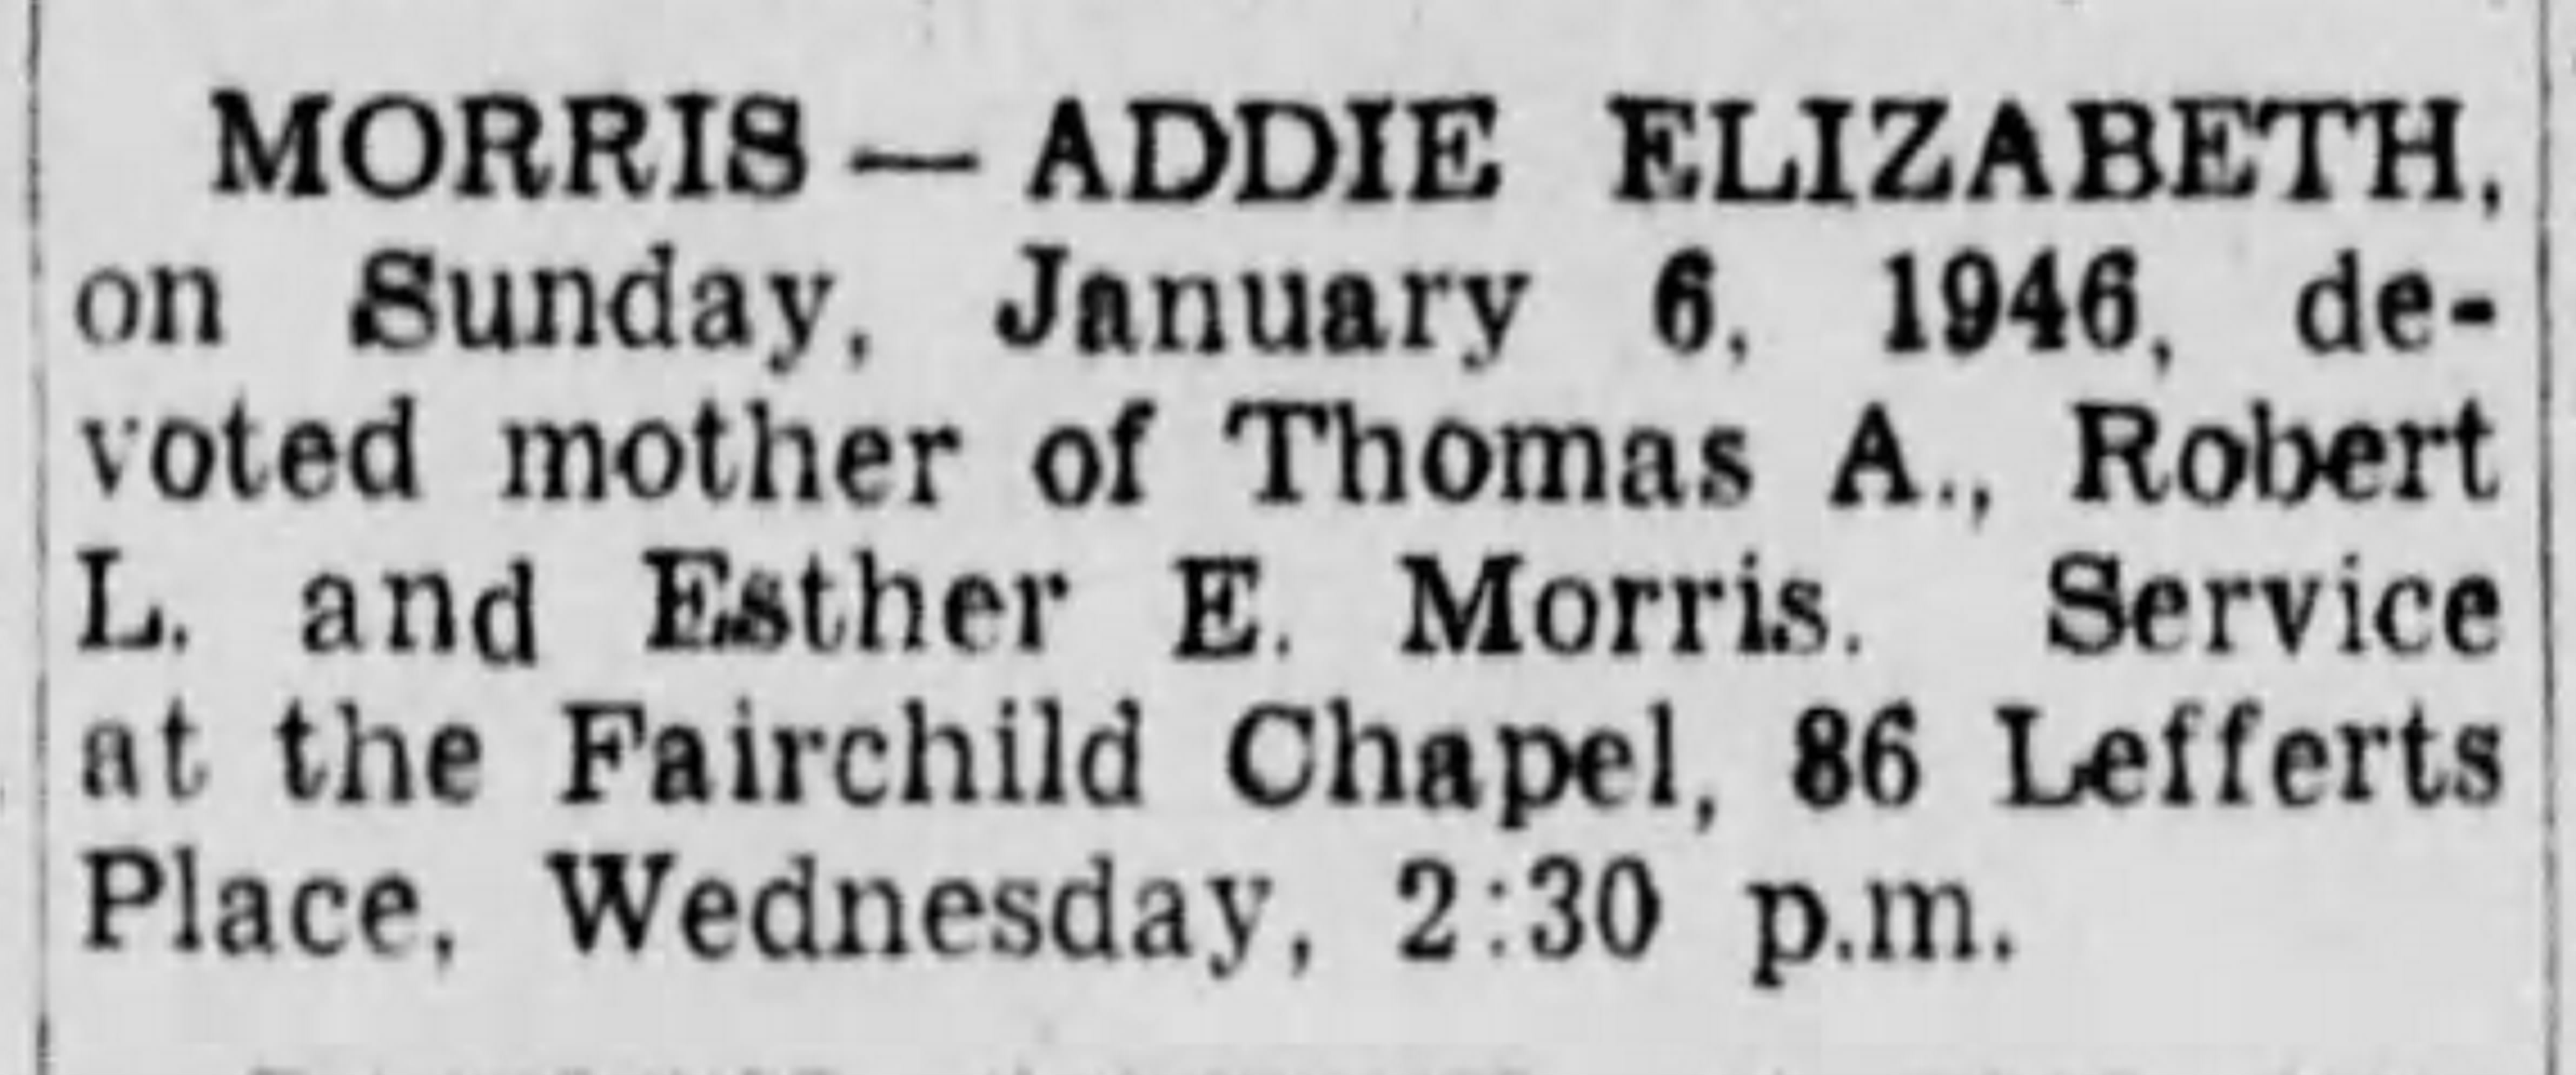
\includegraphics[scale=0.03]{images/The_Brooklyn_Daily_Eagle_Mon__Jan_7__1946_.jpg}
\caption{The death announcement of (Aunt) Addie Morris in the Brooklyn Daily Eagle, printed January 7, 1946, page 7. [Source: \url{http://bklyn.newspapers.com/image/52883100/}, accessed August, 2014]}
\end{figure}

World Horizons exhibit at the 1939 World's Fair: 
http://www.1939nyworldsfair.com/worlds_fair/wf_tour/zone-6/world_horizons/world_horizons.aspx



Next things to search for: 
Walter W.~DeBevoise and candy company

First Methodist Episcopal Church of Morris Park, and Anniversary Day celebrations

Dusenberg's candy store

Commercial High School on Albany Avenue, Brooklyn (and insert picture)

Brooklyn Training School for Teachers

Loomis Sanatorium in Liberty, New York

Export Division's first Transportation Conference (in Detroit newspapers?)

Sayville High School (in 1920s)